%%%%%%%%%%%%%%%%%%%%%%%%%%%%%%%%%%%%%%%%%%%%%%%%%%%%%%%%%%%%%%%%%
% TEMPLATE DE DISSERTAÇÕES E TESES DO PPGIA/PUCPR
% CRIADO POR: JEAN PAUL BARDDAL
% VERSÃO 1 - DEZEMBRO DE 2022
%%%%%%%%%%%%%%%%%%%%%%%%%%%%%%%%%%%%%%%%%%%%%%%%%%%%%%%%%%%%%%%%%

\documentclass{ppgia}

% pt-br ou en-us
\idioma{pt-br}

\title{O Impacto do Sentimento de Notícias Financeiras na Previsão de Direção e Volatilidade do Ativo PETR4: Uma Abordagem via Transformers e Machine Learning}

\author{Vanderlei Barbosa da Silva}
%\studentId{1518036}

% Orientador
\orientador{Prof. Dr. Julio Cesar Nievola}

% Co-orientador, caso exista (se não houver, mantenha comentado com %)
%\coorientador{Nome do(a) Co-orientador(a)}
%\coorientadorUniversidade{Universidade do(a) co-orientador(a)}

%tipo do documento (pdm, msc, pdd, phd)
% pdm = qualificacao de mestrado
% msc = dissertacao completa de mestrado
% pdd = qualificacao de doutorado
% phd = tese completa de doutorado
\tipodocumento{pdm}

% cidade
\cidade{Curitiba}

% universidade (não alterar)
\universidade{Pontifícia Universidade Católica do Paraná}
% programa (não alterar)
\programa{Programa de Pós-Graduação em Informática}
\ano{2026}

% arquivo da ficha catalografica (comentar a linha com % se nao houver ainda)
%\pathfichacatalografica{catalogacao.pdf}

% arquivo da declaracao do programa (comentar a linha com % se não houver ainda)
%\pathdeclaracaoconclusao{declaracao_defesa.pdf}

\graphicspath{{figuras/}}

\usepackage{longtable}
\usepackage{booktabs}

% Nomes em português (a classe não carrega babel): corrige "Figure"/"Table"/"Chapter"
\renewcommand{\figurename}{Figura}
\renewcommand{\tablename}{Tabela}
\renewcommand{\appendixname}{Apêndice}
\renewcommand{\chaptername}{Capítulo}
% \@chapapp é usado pelo cabeçalho de página (\leftmark) e marcadores do PDF
\makeatletter
\renewcommand{\@chapapp}{\chaptername}
\makeatother

\begin{document}
	% Para capa, contra-capa, dedicatória, resumo, abstract, sumário, listas de figuras, ...
	\frontmatter
	
	% Inicia contadores para paginação adequada do restante do documento
	\mainmatter
	
	% Adicione abaixo os capítulos conforme necessário
	\chapter{Introdução} \label{chap:introducao}

A previsão do comportamento de ativos financeiros a partir de informação textual é um dos problemas mais desafiadores na interseção entre a Ciência da Computação e as Finanças. Este capítulo introduz o contexto e a motivação do estudo, define de forma precisa o conceito de sentimento adotado, delimita a lacuna de pesquisa que justifica a investigação e enuncia a questão central, os objetivos e as hipóteses. Ao final, descreve-se a organização dos demais capítulos.

\section{Contextualização e Problematização}

O interesse em compreender o que move os preços das ações é antigo. Já em 1936, Keynes advertia que as oscilações dos mercados não se explicavam apenas por fundamentos econômicos, pois as decisões dos investidores seriam guiadas, em parte, por um impulso psicológico que ele chamou de espírito animal \cite{keynes_general_1936}. Essa intuição perdeu força com a consolidação das teorias racionais de precificação ao longo do século XX, mas retornou ao centro do debate quando se passou a investigar empiricamente o papel da informação na formação dos preços. O estudo pioneiro de \citeonline{cutler_what_1989}, ao perguntar de forma direta o que move os preços das ações, encontrou que os grandes acontecimentos noticiados explicavam uma fração surpreendentemente pequena das variações do mercado. Esse resultado, longe de encerrar a questão, inaugurou uma agenda de pesquisa que persiste até hoje: até que ponto o conteúdo das notícias ajuda a explicar e a antecipar o comportamento dos preços?

Durante boa parte desse percurso, as informações qualitativas, como o teor das notícias, foram tratadas como variáveis latentes, de difícil mensuração, e a pesquisa empírica concentrava-se em dados numéricos. O avanço do Processamento de Linguagem Natural alterou esse quadro ao permitir quantificar o conteúdo textual em larga escala. Duas dimensões do texto passaram a ser estudadas de forma sistemática: a legibilidade, ligada à complexidade da comunicação, e o tom, ou sentimento textual, que diz respeito à carga otimista ou pessimista das palavras empregadas \cite{garcia_sentiment_2013}. É a segunda dimensão, o sentimento, que constitui o objeto desta dissertação, e a sua definição precisa é apresentada adiante.

A compreensão da dinâmica de precificação de ativos no mercado acionário ocupa posição central na literatura financeira há décadas. A Hipótese de Mercados Eficientes (HME), formalizada por \citeonline{fama_efficient_1970}, sustenta que os preços refletem, a cada instante, toda a informação pública disponível. Em sua forma semiforte, a HME prevê que qualquer notícia nova é incorporada ao preço de maneira quase imediata, de modo que a obtenção sistemática de retornos anormais se torna improvável. Para a pesquisa computacional, essa hipótese estabelece um patamar de referência exigente: na ausência de ineficiências exploráveis, a acurácia de qualquer modelo que tente prever a direção diária de um ativo tende a permanecer próxima de 50\%, valor equivalente ao lançamento de uma moeda honesta. Esse patamar será retomado ao longo do texto como critério de avaliação realista dos resultados.

A plausibilidade empírica da eficiência plena foi contestada pelas Finanças Comportamentais. A partir da Teoria do Prospecto de \citeonline{kahneman_prospect_1979}, consolidou-se o entendimento de que os investidores operam sob racionalidade limitada e são influenciados por heurísticas e vieses cognitivos. Esses desvios sistemáticos abrem janelas de ineficiência temporária durante o processo de ajuste dos preços, intervalo em que a informação ainda não foi plenamente incorporada e no qual modelos preditivos podem, em princípio, extrair sinal. Nesse arcabouço, a imprensa especializada cumpre o papel de principal canal de atualização das expectativas. O trabalho de \citeonline{tetlock_giving_2007} foi pioneiro ao quantificar, para o mercado norte-americano, a relação entre o pessimismo veiculado pela mídia e o subsequente movimento de queda dos retornos, acompanhado de elevação da volatilidade.

O mercado acionário brasileiro, operado pela B3, é particularmente permeável a esse fluxo de informação. As ações preferenciais da Petróleo Brasileiro S.A., negociadas sob o código PETR4, constituem um caso ilustrativo. Além de expostas aos choques internacionais do preço do petróleo, essas ações respondem de maneira aguda a intervenções e sinalizações políticas internas, uma vez que a Petrobras é uma empresa de capital misto sob influência do poder público. Essa dupla exposição, ao mercado global de \textit{commodities} e ao ambiente institucional doméstico, faz da PETR4 um objeto rico para investigar como o sentimento das notícias se relaciona ao comportamento dos preços e do risco \cite{silva_o_2018, calomiris_how_2019}.

A modelagem do risco, neste trabalho, apoia-se em uma ferramenta econométrica que convém apresentar desde já, em linhas gerais, para a leitura fluir nos capítulos seguintes. Séries financeiras exibem o fenômeno do agrupamento de volatilidade, em que períodos de grandes oscilações tendem a ser seguidos por novas grandes oscilações, e períodos calmos por novas calmarias. O modelo GARCH (\textit{Generalized Autoregressive Conditional Heteroskedasticity}), proposto por \citeonline{bollerslev_generalized_1986}, captura justamente esse comportamento ao estimar uma variância que varia no tempo em função dos choques recentes e da própria inércia da volatilidade passada. Neste estudo, o GARCH fornece uma medida diária de risco que serve tanto como atributo do modelo preditivo quanto como objeto de avaliação. A formalização completa é apresentada no Capítulo~\ref{chap:metodologia}.

\subsection{Definição operacional de sentimento}

O termo sentimento admite múltiplas acepções, o que torna indispensável fixar a definição empregada nesta dissertação. Adota-se uma definição operacional e quantitativa: sentimento é o escore de polaridade, no intervalo $[-1, +1]$, atribuído ao texto de uma notícia por um modelo de classificação supervisionado. Valores negativos indicam tom pessimista, valores positivos indicam tom otimista e o valor zero indica neutralidade. Essa definição é textual e mensurável, e distingue-se de conceitos correlatos como o humor coletivo de pesquisas de opinião ou o sentimento do investidor inferido de variáveis de mercado. A escolha por uma medida derivada diretamente das manchetes alinha-se ao objetivo de avaliar o conteúdo informacional do noticiário e permite a integração do sinal textual ao modelo quantitativo.

\section{Motivação e Lacuna de Pesquisa}

Do ponto de vista da Ciência da Computação, a extração de sentimento de textos financeiros em português brasileiro permanece um problema aberto. As primeiras abordagens aplicadas ao mercado brasileiro recorreram a técnicas de contagem de palavras, como o \textit{Bag-of-Words} e o TF-IDF, que representam o texto pela frequência dos termos a partir de dicionários predefinidos \cite{nizer_metodo_2011}. Tais técnicas descartam a ordem das palavras e o contexto sintático, o que compromete a interpretação de jargões e de construções ambíguas frequentes no noticiário de mercado. A introdução do Processamento de Linguagem Natural (PLN) baseado no Mecanismo de Atenção, por \citeonline{vaswani_attention_2017}, e do modelo BERT, por \citeonline{devlin_bert_2019}, deslocou o estado da arte para representações contextuais profundas, capazes de ponderar o significado de cada palavra em função das demais. Para o português, o BERTimbau \cite{souza_bertimbau_2020} disponibilizou um modelo de linguagem treinado de forma nativa no idioma. Um modelo de propósito geral, contudo, não constitui, por si só, um classificador de sentimento do domínio financeiro, pois seus dados de treinamento não pertencem majoritariamente a esse domínio. Essa limitação é superada por modelos especializados, como o FinBERT-PT-BR \cite{santos_finbert_2023}, obtido pelo ajuste fino do BERTimbau sobre um amplo corpus financeiro.

A revisão da literatura, detalhada no Capítulo~\ref{chap:referencial_teorico}, evidencia três lacunas que motivam esta pesquisa. A primeira é a escassez de estudos que apliquem modelos de sentimento especializados em finanças ao português brasileiro, em contraste com a abundância de trabalhos voltados ao inglês. A segunda é a ausência de investigações que integrem, em uma arquitetura unificada, três componentes complementares: o sentimento textual contextual, o controle econométrico do risco e a previsão direcional por algoritmos não lineares, aplicados a um ativo específico de elevada sensibilidade política, e não a índices agregados que diluem o risco individual. A terceira é de natureza metodológica e diz respeito à necessidade de assegurar a marcação temporal precisa das notícias, sem a qual a relação causal entre a chegada da informação e a reação do preço não pode ser testada de modo legítimo.

Dois aspectos da literatura recente reforçam a pertinência de investigar especificamente o mercado brasileiro. O primeiro é que o efeito da mídia sobre os preços não é uniforme ao longo do tempo. \citeonline{garcia_sentiment_2013} demonstrou que a reação do mercado ao tom das notícias se concentra nos períodos de recessão, quando os investidores se mostram mais suscetíveis a serem movidos pelo sentimento. O segundo é que esse efeito pode variar entre países. \citeonline{griffin_how_2011} levantaram a hipótese de que, em mercados emergentes, a mídia financeira seria menos influente do que em mercados desenvolvidos, o que torna empiricamente relevante verificar se o sentimento das notícias de fato afeta um ativo de um mercado emergente como o brasileiro. Essa heterogeneidade temporal sugere, ainda, que o efeito do sentimento deva ser examinado não apenas na média, mas ao longo de toda a distribuição do retorno e da volatilidade, perspectiva que esta dissertação incorpora nas análises do Capítulo~\ref{chap:resultados}.

A partir dessas lacunas, formula-se a questão central que orienta o trabalho: de que forma a fusão do sentimento de notícias financeiras, extraído por um modelo \textit{Transformer} especializado em finanças, com a modelagem econométrica do risco pode contribuir para a previsão da direção e da volatilidade do ativo PETR4 na B3?

\section{Objetivos}

\subsection{Objetivo Geral}
Investigar o impacto do sentimento extraído de notícias financeiras, processado por um modelo \textit{Transformer} especializado no domínio financeiro em português, sobre a previsão da direção do preço e da volatilidade do ativo PETR4, por meio de uma arquitetura de fusão de dados com algoritmos de aprendizado de máquina avaliados sob protocolo cronológico que evita o vazamento de informação.

\subsection{Objetivos Específicos}
Cada objetivo específico corresponde a uma etapa necessária do encadeamento metodológico, e a sua razão de ser é explicitada a seguir, conforme recomendado pela banca de qualificação.

\begin{itemize}
    \item Coletar um corpus de notícias financeiras dotado de marcação temporal precisa. Sem a data e a hora exatas de cada publicação, não é possível alinhar de forma causal a notícia ao pregão correspondente, o que inviabiliza qualquer teste da relação de antecedência entre informação e preço. A coleta por meio de interfaces de programação de múltiplos portais atende a esse requisito e, ao diversificar as fontes, reduz o viés associado a um único veículo.
    \item Organizar o corpus segundo uma taxonomia temática supervisionada. A definição prévia de categorias interpretáveis, como notícias da própria empresa, do mercado de petróleo ou de natureza geopolítica, permite analisar separadamente a contribuição de cada vetor de informação e substitui a modelagem não supervisionada de tópicos por uma estrutura auditável e reprodutível.
    \item Extrair o sentimento das notícias por meio de um modelo especializado em finanças. Um classificador ajustado ao domínio reduz o risco de interpretação equivocada de jargões e do sentido econômico do texto, em comparação com modelos genéricos de propósito geral.
    \item Modelar a volatilidade condicional do ativo por um modelo GARCH. O agrupamento de volatilidade é uma regularidade empírica bem documentada das séries financeiras, e a sua modelagem fornece uma medida diária de risco que cumpre dupla função, como atributo preditivo e como objeto de avaliação.
    \item Treinar e avaliar classificadores não lineares sob fusão de dados e divisão cronológica. A previsão direcional requer modelos capazes de capturar relações não lineares, e a avaliação cronológica, com um conjunto de teste consultado uma única vez, assegura que o desempenho medido reflita a capacidade de generalização fora da amostra.
\end{itemize}

\section{Hipóteses da Pesquisa}

A pesquisa parte da premissa de que o fluxo de notícias atua como mecanismo de atualização das expectativas dos investidores. Sobre essa base, formulam-se três hipóteses, apresentadas como proposições a serem testadas, e não como conclusões antecipadas.

\begin{itemize}
    \item \textbf{H1 (Impacto Direcional).} O sentimento textual das notícias, quando fundido aos preços, melhora a previsão da direção dos log-retornos da PETR4 em relação a um modelo que utiliza apenas a informação de preços.
    \item \textbf{H2 (Antecipação de Risco).} O sentimento das notícias antecede a volatilidade condicional da PETR4, exercendo poder preditivo sobre o risco do ativo.
    \item \textbf{H3 (Viés de Negatividade).} Notícias de polaridade negativa associam-se a reações de mercado mais intensas do que notícias positivas de magnitude comparável, em consonância com a assimetria documentada no processamento de informação pelos investidores.
\end{itemize}

Os resultados relativos a cada hipótese, reportados no Capítulo~\ref{chap:resultados}, têm magnitude compatível com a quase-eficiência do mercado, e a sua interpretação é conduzida com a cautela que a HME impõe.

\section{Justificativa e Relevância}

No plano acadêmico, a dissertação contribui para a interseção entre as Finanças Comportamentais e a Ciência de Dados ao avaliar de forma empírica um modelo de linguagem especializado em finanças no português brasileiro, evitando a perda de informação que decorre da tradução de dicionários estrangeiros \cite{henrique_literature_2019}. Como a maior parte da produção quantitativa se concentra no mercado norte-americano e na língua inglesa, a aplicação dessas técnicas ao contexto da B3, e especificamente a um ativo de elevada sensibilidade política, ajuda a preencher uma lacuna geográfica e idiomática.

No plano prático, o estudo entrega uma arquitetura reprodutível que integra a volatilidade econométrica à semântica contextual de domínio para a análise de risco. Os resultados, reportados com transparência quanto à sua magnitude e à sua significância estatística, oferecem subsídios para o entendimento do papel informacional da mídia na precificação da PETR4, sem que se atribua ao método capacidade preditiva além da que foi efetivamente medida.

\section{Organização do Documento}

Os capítulos seguintes estão organizados da forma descrita a seguir. O Capítulo~\ref{chap:referencial_teorico} apresenta o referencial teórico e a Revisão Sistemática da Literatura, com a \textit{string} de busca, a janela temporal, os critérios de seleção e a discussão dos trabalhos correlatos, posicionando a originalidade do estudo. O Capítulo~\ref{chap:metodologia} distingue a metodologia, isto é, a natureza e os pressupostos da pesquisa, do método propriamente dito, descrevendo a coleta de dados com marcação temporal, a taxonomia, a extração de sentimento, a modelagem do risco e a fusão de dados, e ilustra o percurso completo com um exemplo. O Capítulo~\ref{chap:resultados} reporta e discute os resultados obtidos sobre o corpus completo, incluindo os testes de significância, a análise de causalidade e a avaliação da volatilidade. O Capítulo~\ref{chap:conclusao} sintetiza as conclusões, examina as limitações, discute a generalização para outros ativos e aponta os desdobramentos futuros.

	\chapter{Referencial Teórico} \label{chap:referencial_teorico}

A pesquisa proposta nesta dissertação situa-se em um ponto de encontro entre duas tradições intelectuais que, por muito tempo, caminharam separadas. De um lado está a teoria financeira, preocupada em entender como os preços dos ativos se formam e como a informação se incorpora a eles. De outro está a Ciência da Computação, que oferece os instrumentos para representar e interpretar a linguagem humana em escala. Este capítulo costura essas duas tradições. Começa pela discussão teórica que justifica a própria possibilidade de extrair sinal preditivo de notícias, percorre o papel da mídia na formação de expectativas, examina a especificidade do ativo estudado, reconstrói a evolução das técnicas de Processamento de Linguagem Natural aplicadas a finanças, apresenta os fundamentos econométricos do risco e da fusão de dados e, ao final, sistematiza a literatura correlata por meio de uma revisão estruturada. A intenção é que, ao término da leitura, fique claro não apenas o que já foi feito, mas sobretudo onde se encontra a lacuna que este trabalho pretende preencher.

\section{A Hipótese de Mercados Eficientes}

O ponto de partida obrigatório de qualquer estudo sobre previsibilidade de preços é a Hipótese de Mercados Eficientes. Em sua formulação clássica, devida a \citeonline{fama_efficient_1970}, um mercado é eficiente quando os preços dos ativos refletem, a todo instante, a totalidade da informação disponível. A consequência dessa definição é severa para quem deseja prever retornos: se toda a informação já está no preço, então as variações futuras dependem apenas de informação ainda não revelada, que por definição é imprevisível. O preço passa a se comportar como um passeio aleatório, e a melhor estimativa para o valor de amanhã é o valor de hoje.

A teoria distingue três formas de eficiência, conforme a amplitude do conjunto informacional considerado. Na forma fraca, os preços incorporam apenas o histórico de cotações, de modo que a análise técnica baseada em padrões passados não geraria retornos anormais. Na forma semiforte, os preços refletem também toda a informação pública, o que inclui notícias, balanços e anúncios corporativos. Na forma forte, incorporam ainda a informação privada de agentes com acesso privilegiado. É a forma semiforte que interessa de maneira direta a esta dissertação, pois é nela que se coloca a questão central: o conteúdo de uma notícia financeira é absorvido pelos preços de modo instantâneo, ou resta, por algum intervalo mensurável, um resíduo de previsibilidade que um modelo computacional poderia explorar?

A hipótese, em sua versão mais rígida, não resistiu intacta ao escrutínio empírico. \citeonline{shiller_stock_1981} mostrou que os preços das ações oscilam muito mais do que seria justificável pelas variações nos dividendos futuros, sugerindo a presença de uma volatilidade em excesso incompatível com a racionalidade plena. Estudos posteriores documentaram anomalias persistentes. \citeonline{de_bondt_does_1985} encontraram evidência de que o mercado reage de forma exagerada a notícias, com reversões previsíveis no longo prazo, ao passo que \citeonline{jegadeesh_returns_1993} identificaram o efeito de momento, segundo o qual ativos que subiram tendem a continuar subindo por alguns meses. Diante desse acúmulo de evidências, mesmo defensores da hipótese passaram a admitir uma versão mais branda. \citeonline{malkiel_efficient_2003} reconhece que os mercados não são perfeitamente eficientes, mas argumenta que as ineficiências são pequenas, transitórias e difíceis de explorar depois de descontados os custos. É justamente nessa zona de quase-eficiência que esta pesquisa se posiciona: não se supõe a existência de um sinal forte e estável, e sim a possibilidade de um sinal fraco, porém real, capaz de deslocar a acurácia de um preditor alguns pontos percentuais acima do acaso.

Convém traduzir essas formas em termos operacionais para a tarefa preditiva desta dissertação. Sob a forma fraca, um preditor que use apenas o histórico de preços não deveria superar o acaso; sob a forma semiforte, tampouco um preditor que incorpore notícias públicas o faria de modo persistente. A previsão da direção diária de um ativo é, por isso, um teste exigente da própria hipótese: um desempenho sistematicamente acima de cinquenta por cento, ainda que por margem estreita, constitui evidência de ineficiência informacional explorável. É essa a régua adotada ao longo do trabalho, e por ela se deve julgar a magnitude, e não apenas o sinal, dos resultados. Cabe ressaltar, ademais, que mesmo um sinal estatisticamente real pode não ser economicamente explorável uma vez descontados os custos de transação. Essa distinção entre significância estatística e significância econômica, central à crítica de \citeonline{malkiel_efficient_2003} às anomalias, é honrada nesta dissertação ao se avaliar, além das métricas estatísticas, o desempenho de uma estratégia de negociação líquida de custos.

A defesa da eficiência não permaneceu inerte diante das anomalias. \citeonline{fama_market_1998} argumentou que muitas delas seriam fruto de metodologia ou de acaso, e que se distribuiriam de forma equilibrada entre reações exageradas e reações insuficientes, o que seria compatível com a eficiência. A controvérsia, longe de ser estéril, deslocou o debate para o conceito de limites à arbitragem. \citeonline{delong_noise_1990} demonstraram que a presença de investidores de ruído, que negociam com base em sentimento e não em fundamentos, pode afastar os preços do valor justo e, sobretudo, que o risco imposto por esses próprios investidores desencoraja os arbitradores racionais de corrigir o desvio. Disso resulta que as ineficiências podem persistir, e que o sentimento, longe de ser irrelevante, converte-se em um fator de risco com consequências sobre os preços. Essa perspectiva fornece o elo teórico entre a existência de um sinal de sentimento explorável e a sua natureza necessariamente limitada, coerente com a magnitude modesta dos efeitos que esta dissertação viria a documentar. Uma síntese acessível dessa transição, da teoria dos mercados eficientes para as finanças comportamentais, é oferecida por \citeonline{shiller_efficient_2003}.

\section{O Teorema da Concordância e o Papel da Informação}

Uma questão precede logicamente a discussão sobre o impacto das notícias: por que, afinal, a informação pública deveria mover os preços e gerar negociação? Uma resposta formal vem do teorema da concordância de \citeonline{aumann_agreeing_1976}, conhecido pela expressão concordar em discordar. Aumann demonstrou que, se dois agentes racionais partem de uma mesma probabilidade a priori e atualizam suas crenças pela regra de Bayes, e se as suas probabilidades a posteriori sobre um evento são de conhecimento comum, então essas probabilidades devem necessariamente coincidir. Em outras palavras, agentes plenamente racionais e com conhecimento comum não podem, de forma consistente, concordar em discordar sobre a probabilidade de um evento.

O teorema tem uma implicação importante para esta pesquisa. Se todos os investidores fossem perfeitamente racionais e compartilhassem o mesmo conjunto de informações, haveria pouca razão para negociar, pois as discordâncias tenderiam a se dissolver. O fato de existir intenso volume de negociação, e de os preços reagirem à chegada de notícias, indica que os investidores partem de crenças heterogêneas e processam a informação de maneiras distintas. A notícia pública funciona, nesse arcabouço, como o sinal que atualiza as probabilidades a posteriori dos agentes, e a forma como cada investidor interpreta o seu tom, otimista ou pessimista, ajuda a explicar a revisão das expectativas e o consequente movimento dos preços. Esse raciocínio foi levado ao limite por \citeonline{milgrom_information_1982}, cujo teorema da não-negociação demonstra que, partindo de crenças comuns e com racionalidade plena, a simples disposição de um agente a negociar revelaria informação privada e desencorajaria a contraparte, de modo que não haveria troca por motivo puramente especulativo. O enorme volume de negociação observado na prática é, portanto, um paradoxo sob a racionalidade estrita, e a sua explicação requer ou crenças heterogêneas, ou motivações de liquidez, ou desvios comportamentais. As notícias atuam exatamente sobre o primeiro desses canais, ao alimentar interpretações divergentes de um mesmo fato. O teorema da concordância e o seu corolário de não-negociação fornecem, assim, um fundamento racional para tratar o sentimento das notícias como informação economicamente relevante, que se soma à leitura comportamental apresentada na seção seguinte.

\section{Finanças Comportamentais}

Se a Hipótese de Mercados Eficientes fornece o pano de fundo, são as Finanças Comportamentais que fornecem o mecanismo pelo qual a informação textual poderia ter valor preditivo. Essa corrente parte de uma constatação simples e poderosa: os seres humanos não processam a informação como autômatos bayesianos perfeitos.

O marco fundador é a Teoria do Prospecto de \citeonline{kahneman_prospect_1979}, que demonstrou, por meio de experimentos, que as pessoas avaliam ganhos e perdas em relação a um ponto de referência, e não em termos de riqueza absoluta, e que sentem as perdas com intensidade maior do que os ganhos equivalentes. Esse fenômeno, conhecido como aversão à perda, tem uma implicação direta para o mercado: a reação a uma notícia ruim tende a ser mais aguda do que a reação a uma notícia boa de mesma magnitude. Em trabalho anterior, \citeonline{tversky_judgment_1974} já haviam catalogado um conjunto de heurísticas, como a representatividade, a disponibilidade e a ancoragem, que levam a desvios sistemáticos do julgamento sob incerteza.

A Teoria do Prospecto descreve esse comportamento por meio de uma função de valor com três propriedades que importam ao estudo das notícias. A função é definida sobre ganhos e perdas relativos a um ponto de referência, e não sobre a riqueza absoluta; é côncava no domínio dos ganhos e convexa no dos perdas, o que reflete a aversão ao risco diante de ganhos e a propensão ao risco diante de perdas; e é mais inclinada do lado das perdas, traduzindo numericamente a aversão à perda. A essa função soma-se uma ponderação não linear das probabilidades, que faz com que eventos raros, como grandes quedas, recebam peso desproporcional na decisão. Em conjunto, essas propriedades preveem que o investidor reagirá de modo assimétrico e mais intenso à informação negativa, fundamento microeconômico direto da hipótese de assimetria que esta dissertação testa empiricamente.

Os desvios não se limitam ao indivíduo isolado. No plano coletivo, o comportamento de manada leva os investidores a imitar as decisões alheias, amplificando movimentos iniciados por notícias e gerando bolhas e quedas abruptas. O efeito de disposição, por sua vez, descreve a tendência a vender cedo demais os ativos vencedores e a reter por tempo excessivo os perdedores, o que distorce a reação aos fundamentos. Tomados em conjunto, esses fenômenos sustentam a tese de que o fluxo de notícias, ao alimentar emoções e heurísticas, exerce sobre os preços um efeito que a racionalidade plena não preveria, efeito cuja intensidade e cujo sinal esta pesquisa procura quantificar.

Transposta para o agregado do mercado, a aversão à perda ajuda a explicar o chamado viés de negatividade, central para a terceira hipótese desta dissertação. Esse viés tem raízes cognitivas profundas: a psicologia documenta que eventos negativos exercem impacto maior do que eventos positivos de igual magnitude, princípio sintetizado na ideia de que o ruim é mais forte do que o bom \cite{baumeister_bad_2001, rozin_negativity_2001}. No plano da linguagem, isso se reflete em um vocabulário mais rico para descrever aspectos negativos, e os próprios léxicos de sentimento financeiro, como o de \citeonline{loughran_when_2011}, são compostos majoritariamente por termos negativos. Notícias de tom pessimista parecem provocar movimentos de preço e, sobretudo, picos de volatilidade mais intensos do que notícias otimistas. \citeonline{corredor_investor_2013} confirmaram essa assimetria em quatro mercados europeus e mostraram que a sua intensidade varia conforme características dos ativos e fatores culturais e institucionais de cada país, o que sugere que o efeito não é universal, mas dependente do contexto. No Brasil, \citeonline{silva_o_2018} ofereceu evidência convergente ao documentar que o sentimento das notícias afeta tanto o retorno quanto a volatilidade das ações.

O conceito de sentimento do investidor ganhou, com o tempo, estatuto próprio na literatura. \citeonline{baker_investor_2007} argumentaram que ondas de otimismo e pessimismo, difíceis de justificar por fundamentos, influenciam de modo sistemático os preços, em especial os de ações mais difíceis de arbitrar, como as de empresas pequenas, jovens ou voláteis. A PETR4, embora seja um papel de grande capitalização, compartilha um traço que a torna sensível a essas ondas: a sua forte exposição a fatores políticos, que alimentam narrativas e humores de mercado pouco ancorados em fundamentos estáveis.

\subsection{Modelos de reação e o papel da atenção}

A pesquisa comportamental não se limitou a catalogar vieses; propôs modelos formais que conciliam a evidência de reação exagerada no longo prazo com a de reação insuficiente no curto prazo. \citeonline{barberis_model_1998} construíram um modelo em que os investidores, ao alternarem entre regimes de crença, ora subreagem ora sobre-reagem às notícias, o que gera, respectivamente, momento de curto prazo e reversão de longo prazo. Em linha complementar, \citeonline{daniel_investor_1998} derivaram padrões semelhantes a partir do excesso de confiança e da atribuição enviesada, segundo os quais os investidores superestimam a precisão de sua informação privada. Esses modelos são relevantes para esta dissertação porque preveem que a reação do mercado ao conteúdo das notícias depende do horizonte e do estado de crença, o que motiva a análise do efeito do sentimento ao longo da distribuição do retorno, e não apenas na sua média.

Um segundo mecanismo, a atenção limitada, ajuda a explicar por que as notícias movem os preços mesmo quando não trazem fundamentos inteiramente novos. \citeonline{barber_all_2008} mostraram que ativos que ganham destaque na mídia atraem desproporcionalmente a atenção dos investidores individuais, gerando pressão de compra e movimentos de preço. A cobertura jornalística atua, portanto, não apenas como veículo de informação, mas como alocador de atenção, dimensão particularmente pertinente para um ativo de grande visibilidade midiática como a PETR4. Uma sistematização ampla desses mecanismos psicológicos e de seus efeitos sobre a precificação é apresentada por \citeonline{hirshleifer_investor_2001}. A Tabela~\ref{tab:vieses} resume os principais vieses e a sua implicação para o estudo do sentimento.

\begin{table}[htpb]
\centering
\caption{Principais vieses comportamentais e suas implicações para o efeito do sentimento das notícias.}
\label{tab:vieses}
\resizebox{0.98\textwidth}{!}{%
\begin{tabular}{p{3.2cm} p{5.4cm} p{5.6cm}}
\hline
\textbf{Viés} & \textbf{Descrição} & \textbf{Implicação para o sentimento} \\ \hline
Aversão à perda & As perdas pesam mais do que ganhos equivalentes & Reação assimétrica, mais intensa a notícias negativas \\
Excesso de confiança & Superestimação da precisão da própria informação & Sobre-reação às notícias, com reversão posterior \\
Atenção limitada & Capacidade restrita de processar a informação disponível & Notícias em destaque movem os preços por saliência \\
Ancoragem & Apego a valores de referência iniciais & Ajuste lento e incompleto às novas informações \\
Comportamento de manada & Imitação das decisões dos demais agentes & Amplificação dos efeitos do sentimento coletivo \\ \hline
\end{tabular}%
}
\vspace{0.2cm}
{\small \\ Fonte: Elaborado pelo autor com base na literatura citada.}
\end{table}

\section{A Mídia como Vetor de Informação}

Estabelecido que os investidores são sensíveis ao tom da informação, resta entender por qual canal essa informação chega até eles. A imprensa especializada é o canal por excelência, e a quantificação do seu efeito é o que aproxima as Finanças Comportamentais da computação.

O estudo seminal nessa direção é o de \citeonline{tetlock_giving_2007}, que construiu um índice de pessimismo a partir de uma coluna diária do \textit{Wall Street Journal} e mostrou que valores elevados de pessimismo antecedem quedas nos retornos do mercado, seguidas de uma reversão à média, além de se associarem a aumentos no volume negociado. O trabalho é importante por dois motivos. Primeiro, porque tratou o texto jornalístico como uma fonte de dados quantificável. Segundo, porque ofereceu uma interpretação econômica coerente com a teoria, na qual o pessimismo da mídia funciona como um indicador de sentimento que move temporariamente os preços para longe do seu valor fundamental.

A virada para as mídias sociais ampliou enormemente o volume de texto disponível. \citeonline{bollen_twitter_2011} mostraram que dimensões do humor coletivo extraídas de mensagens do Twitter antecipavam variações do índice Dow Jones, com ganho de acurácia na previsão direcional. \citeonline{antweiler_is_2004} já haviam investigado fóruns de discussão financeira e concluído que, embora boa parte do conteúdo seja ruído, há informação genuína capaz de prever volatilidade e volume. Na mesma linha, \citeonline{nguyen_sentiment_2015} incorporaram sentimentos associados a tópicos específicos extraídos de fóruns e obtiveram melhora sobre modelos baseados apenas em preços, reforçando a ideia de que o conteúdo temático, e não apenas a polaridade média, carrega sinal.

A natureza do efeito também foi esmiuçada em diferentes horizontes e fontes. \citeonline{li_effect_2014} analisaram o impacto conjunto de notícias corporativas e do humor público sobre os movimentos das ações e constataram que esse impacto varia conforme as características da empresa e o conteúdo da notícia. Em frequência ainda mais fina, \citeonline{gros-klusmann_when_2011} mediram intradiariamente a reação do mercado à leitura automatizada de notícias e mostraram que o ajuste de preços ocorre em minutos, o que torna a marcação temporal precisa um requisito incontornável para qualquer teste sério de causalidade. Esse achado antecipa, na literatura internacional, a exigência metodológica que se tornou o eixo da presente dissertação.

O efeito da mídia não é homogêneo entre países. \citeonline{calomiris_how_2019} analisaram um amplo painel internacional e concluíram que o fluxo de notícias e o seu contexto influenciam risco e retorno de forma estruturalmente mais severa em mercados emergentes do que em mercados desenvolvidos, o que se atribui à maior incerteza institucional e à menor profundidade desses mercados. Para o caso brasileiro, \citeonline{cardoso_whats_nodate} examinaram o impacto das manchetes sobre a atividade econômica nacional e evidenciaram a sensibilidade do ambiente de negócios ao noticiário, resultado que ampara a escolha do Brasil como objeto de estudo.

O acúmulo dessas evidências consolidou a análise textual como um campo próprio dentro das finanças, hoje sistematizado em revisões abrangentes \cite{kearney_textual_2014, loughran_textual_2016}. Desde os primeiros sistemas de extração de sentimento de fóruns na internet \cite{das_yahoo_2007}, a área amadureceu a ponto de separar o conteúdo informativo da notícia em si do sentimento que a acompanha. \citeonline{heston_news_2017}, por exemplo, mostraram que, mesmo controlando pela ocorrência da notícia, o seu tom ainda carrega poder preditivo sobre os retornos, o que reforça a pertinência de medir o sentimento de forma autônoma, tal como se faz nesta dissertação.

\section{A PETR4 e a Distinção entre Mercado e Ativo}

A escolha da PETR4 como objeto não é arbitrária, e a sua compreensão exige uma digressão sobre a economia do petróleo. As ações preferenciais da Petrobras reúnem, em um único papel, duas fontes de risco que nem sempre apontam na mesma direção.

A primeira fonte é o mercado internacional de petróleo. Como produtora da \textit{commodity}, a Petrobras tem suas receitas atadas ao preço do barril. A literatura econômica há muito investiga a relação entre o preço do petróleo e a economia. \citeonline{hamilton_oil_1983} documentou que quase todas as recessões norte-americanas do pós-guerra foram precedidas por elevações no preço do petróleo, estabelecendo o papel macroeconômico desses choques. Décadas depois, \citeonline{kilian_not_2009} refinou essa compreensão ao mostrar que nem todos os choques de preço do petróleo são iguais: é preciso distinguir choques de oferta, associados a interrupções de produção, de choques de demanda, ligados ao aquecimento da atividade global. Essa distinção tem uma consequência crucial para a presente pesquisa. Um evento geopolítico que reduza a oferta e eleve o preço do barril pode beneficiar a receita de uma produtora, ainda que represente uma má notícia para a economia como um todo e para o índice de ações. O mecanismo de transmissão é assimétrico conforme a origem do choque. Um choque de oferta, como o fechamento de uma rota de transporte ou um corte de produção, eleva o preço do petróleo e tende a aumentar a margem de uma produtora integrada, ao passo que um choque de demanda negativo, como uma recessão global que reduz o consumo, derruba simultaneamente o preço da \textit{commodity} e a atividade, prejudicando a empresa por duas vias. Para um índice amplo de ações, ambos os choques costumam ser desfavoráveis; para uma produtora de petróleo, porém, o primeiro pode ser favorável. É exatamente essa não trivialidade que torna inadequado tratar toda notícia de tom negativo sobre petróleo como sinal de queda para a PETR4, e que justifica o tratamento diferenciado por categoria temática adotado no método.

A segunda fonte de risco é política. Por ser uma empresa de capital misto, sob influência do Estado, a Petrobras tem suas decisões de preço, investimento e governança permeadas por considerações políticas. Isso a transforma em uma espécie de termômetro do risco institucional brasileiro, à semelhança do que \citeonline{baker_investor_2007} descrevem para ativos suscetíveis ao sentimento.

Da combinação dessas duas fontes emerge o ponto que a banca de qualificação levantou com precisão e que esta dissertação incorpora de forma explícita: uma notícia negativa para o mercado em geral não é necessariamente negativa para a PETR4 em particular. Uma guerra no Oriente Médio que derrube as bolsas mundiais pode, ao elevar o preço do petróleo, favorecer a produtora nacional. Tratar todo tom negativo como sinal de queda do ativo seria, portanto, um erro de interpretação econômica. A solução adotada no método, descrita no Capítulo~\ref{chap:metodologia}, é a organização das notícias por uma taxonomia temática que separa eventos da empresa de eventos do mercado de petróleo, permitindo que o sentido econômico de cada categoria seja considerado.

\section{Incerteza Econômica como Condicionante}

A literatura sugere que o efeito das notícias sobre os preços não é constante, e sim mais intenso em períodos de turbulência. Para tratar essa heterogeneidade de forma rigorosa, é necessário precisar o conceito de incerteza econômica. A distinção seminal é a de \citeonline{knight_risk_1921}, que separou risco de incerteza: o risco refere-se a situações em que a distribuição de probabilidade dos resultados é conhecida, ao passo que a incerteza, em sentido estrito, descreve situações em que essa distribuição é desconhecida. \citeonline{bloom_fluctuations_2014} associa a incerteza às dúvidas dos agentes sobre o futuro, relacionando-a a fenômenos macroeconômicos e microeconômicos, enquanto \citeonline{jurado_measuring_2015} a operacionalizam como a volatilidade condicional da parcela imprevisível das expectativas.

Como a incerteza não é diretamente observável, a literatura recorre a aproximações. Uma das mais influentes é o índice de incerteza de política econômica de \citeonline{baker_measuring_2016}, construído, de forma sugestiva para esta pesquisa, a partir da frequência de termos relacionados à incerteza em jornais, o que evidencia que o próprio texto noticioso carrega informação sobre o estado de incerteza da economia. A relevância desse conceito para a presente dissertação é dupla. Primeiro, porque a evidência de que o sentimento das notícias afeta mais os preços em períodos de recessão \cite{garcia_sentiment_2013} sugere que o seu poder preditivo deve ser avaliado de modo sensível ao regime de mercado. Segundo, porque a própria volatilidade condicional estimada pelo GARCH funciona como uma aproximação do nível de incerteza do mercado, o que liga diretamente a modelagem de risco à análise do sentimento. Essa articulação motiva as análises por subperíodo e por regime conduzidas no Capítulo~\ref{chap:resultados}.

\section{Processamento de Linguagem Natural em Finanças}

A capacidade de transformar texto em sinal numérico é o que viabiliza tudo o que foi discutido até aqui. Esta seção reconstrói a evolução dessa capacidade em quatro estágios sucessivos, cada um superando limitações do anterior.

\subsection{A distribuição das palavras: a Lei de Zipf}

Antes de representar um texto numericamente, é útil compreender uma regularidade estatística da linguagem que condiciona todas as técnicas de mineração textual. Ao estudar a frequência das palavras em obras literárias, \citeonline{zipf_human_1949} observou que a frequência de uma palavra é aproximadamente inversamente proporcional à sua posição em um \textit{ranking} de ocorrências, de modo que o produto entre a frequência e a posição permanece quase constante. Essa regularidade, conhecida como lei de Zipf, implica que poucas palavras são extremamente frequentes, enquanto a imensa maioria do vocabulário ocorre muito raramente. Para as palavras de baixa frequência, \citeonline{booth_law_1967} formulou uma lei complementar.

A lei de Zipf tem consequências diretas para a análise de sentimento. De um lado, as palavras mais frequentes tendem a ser conectivos e termos genéricos, de baixo poder discriminante, o que justifica a sua remoção ou o seu rebaixamento por esquemas de ponderação como o TF-IDF. De outro, o conteúdo informativo concentra-se em termos relativamente raros e específicos do domínio, o que explica por que as representações baseadas apenas em contagem enfrentam o problema da esparsidade, e por que modelos contextuais, capazes de inferir o significado de uma palavra a partir de poucas ocorrências e do seu entorno, representam um avanço. Essa compreensão fundamenta tanto a construção da taxonomia de termos adotada no método quanto a opção por um modelo de linguagem contextual.

A Figura~\ref{fig:zipf} confirma a validade da lei de Zipf no corpus desta pesquisa. Ao ordenar as palavras das notícias da PETR4 pela frequência e plotar a frequência contra a posição em escala logarítmica, obtém-se uma reta descendente próxima da curva teórica, o que evidencia que pouquíssimas palavras concentram a maior parte das ocorrências, enquanto a vasta maioria do vocabulário, de mais de quarenta mil palavras distintas, aparece raramente.

\begin{figure}[htpb]
\centering
\caption{Distribuição de frequência das palavras no corpus de notícias da PETR4, em escala logarítmica, comparada à curva teórica da lei de Zipf. A aderência confirma a concentração das ocorrências em poucos termos.}
\vspace{0.2cm}
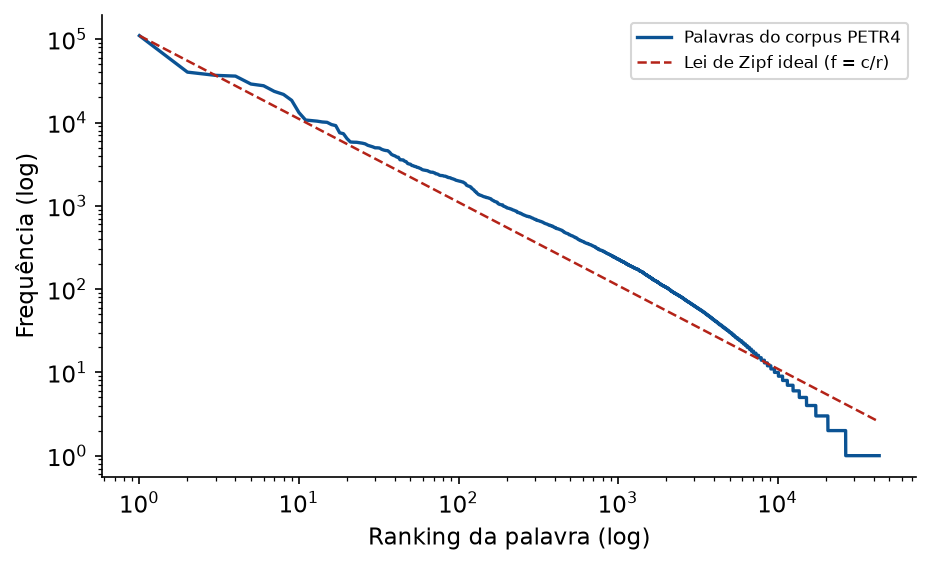
\includegraphics[width=0.75\textwidth]{figuras/fig_zipf.png}
\label{fig:zipf}
\vspace{0.2cm}
{\small Fonte: Elaborado pelo autor.}
\end{figure}

\subsection{Representações léxicas e de contagem}

As primeiras aplicações representavam um documento como um vetor de frequências de palavras, abordagem conhecida como \textit{Bag-of-Words}. A variante mais difundida, o TF-IDF, pondera cada termo pela sua frequência no documento e pela sua raridade no conjunto, de modo a destacar palavras discriminantes. No mercado brasileiro, \citeonline{nizer_metodo_2011} foi precursor ao empregar essa família de técnicas para detectar o efeito de publicações de notícias sobre ações da Bovespa, em um trabalho que abriu caminho para a pesquisa nacional na área.

Para tornar a contagem sensível ao domínio, desenvolveram-se léxicos de sentimento, isto é, listas de palavras previamente classificadas como positivas ou negativas. A contribuição decisiva nessa linha foi a de \citeonline{loughran_when_2011}, que demonstraram que dicionários de uso geral classificam de forma equivocada o vocabulário financeiro: termos como passivo, custo ou imposto, neutros ou meramente técnicos em finanças, seriam contados como negativos por um léxico genérico. A construção de um dicionário financeiro específico, hoje referência consolidada na área, corrigiu esse viés e melhorou substancialmente a medição do tom. Ainda assim, todos os métodos dessa família partilham a limitação estrutural já apontada: ao representar o texto como um conjunto de palavras independentes, ignoram a negação, a ironia e a dependência de contexto, de modo que as frases resultado acima do esperado e resultado abaixo do esperado, que diferem em uma única palavra mas têm sentidos opostos, podem receber tratamento semelhante. A superação dessa limitação foi o motor da evolução descrita nas subseções seguintes.

O reconhecimento de que o vocabulário financeiro tem conotações próprias levou ao desenvolvimento de léxicos especializados. \citeonline{loughran_when_2011} demonstraram que listas de palavras negativas de uso geral classificam erroneamente muitos termos no contexto financeiro, pois palavras como passivo ou imposto não carregam, nesse domínio, a carga negativa que teriam em outro. A criação de um dicionário financeiro específico melhorou de forma sensível a análise. Ainda assim, todas essas representações compartilham uma limitação de fundo: ao tratar o texto como um saco de palavras, descartam a ordem e a sintaxe, o que as torna incapazes de interpretar negações, ironias e construções dependentes do contexto, frequentes no jornalismo de mercado.

\subsection{Aprendizado de máquina e seleção de atributos}

O estágio seguinte associou as representações textuais a classificadores de aprendizado de máquina, capazes de aprender fronteiras de decisão a partir de exemplos. \citeonline{schumaker_quantitative_2009} construíram o sistema AZFinText, que combinou informação de preços a atributos textuais por meio de máquinas de vetores de suporte e foi um dos primeiros sistemas quantitativos de previsão baseados em notícias a apresentar resultados de negociação simulada. \citeonline{hagenau_automated_2013} avançaram ao mostrar que atributos sensíveis ao contexto das sentenças, e não apenas a contagem isolada de palavras, elevam a acurácia da previsão.

À medida que o número de atributos textuais cresce, surge o problema da alta dimensionalidade, que prejudica o desempenho dos classificadores. \citeonline{odhiambo_omuya_feature_2021} enfrentaram esse problema com técnicas de seleção de atributos baseadas em ganho de informação, obtendo modelos mais enxutos e precisos. No tocante à escolha do algoritmo, \citeonline{ballings_evaluating_2015} conduziram uma avaliação extensa de múltiplos classificadores para a previsão direcional binária e apontaram métodos baseados em árvores e em margens, como o \textit{Random Forest} e as máquinas de vetores de suporte, entre os mais adequados, conclusão que ampara a escolha dos classificadores empregados nesta dissertação. Arquiteturas híbridas, que combinam componentes lineares e não lineares, também se mostraram úteis, como demonstrou \citeonline{wang_stock_2012} ao mesclar modelos de séries temporais a redes neurais para a previsão de índices. O problema da alta dimensionalidade, conhecido como maldição da dimensionalidade, é particularmente agudo na análise textual, pois o vocabulário de um corpus pode conter dezenas de milhares de termos, cada um dando origem a um atributo. Nesse regime, o número de atributos rivaliza ou supera o número de observações, o que facilita o sobreajuste e degrada a generalização. As respostas a esse problema seguem duas direções complementares: a seleção de atributos, que descarta os termos pouco informativos, e a redução de dimensionalidade, que projeta os atributos em um espaço menor. A taxonomia temática adotada nesta dissertação pode ser entendida como uma forma supervisionada e interpretável de redução de dimensionalidade, na qual milhares de termos possíveis são condensados em sete dimensões de sentimento, uma por categoria, sem a perda de interpretabilidade que acompanharia uma projeção puramente estatística.

\subsection{Representações distribuídas de palavras}

Um avanço intermediário entre a contagem de palavras e os modelos contextuais foi a introdução das representações distribuídas, conhecidas como \textit{word embeddings}. Em vez de tratar cada palavra como um símbolo isolado, esses métodos a representam por um vetor denso, aprendido de modo que palavras de significado semelhante ocupem posições próximas no espaço vetorial. O modelo \textit{word2vec}, de \citeonline{mikolov_efficient_2013}, e o \textit{GloVe}, de \citeonline{pennington_glove_2014}, popularizaram essa ideia ao aprender vetores a partir de grandes corpora, capturando relações semânticas e sintáticas que a representação \textit{Bag-of-Words} ignora. Os \textit{embeddings} atenuaram o problema da esparsidade apontado pela lei de Zipf, mas ainda atribuíam a cada palavra um único vetor, independentemente do contexto, limitação que só seria plenamente superada pelos modelos contextuais discutidos a seguir.

\subsection{Aprendizado profundo}

A terceira virada veio com o aprendizado profundo, que dispensou a engenharia manual de atributos ao aprender representações diretamente dos dados. As redes neurais convolucionais, originalmente concebidas para imagens, foram adaptadas ao texto ao deslizar filtros sobre sequências de palavras, detectando padrões locais como expressões e combinações de termos relevantes, independentemente da posição em que ocorrem na frase. As redes recorrentes, por sua vez, processam a sequência elemento a elemento e mantêm um estado interno que resume o que foi lido, modelando a dependência entre as palavras. \citeonline{vargas_deep_2017} aplicaram essa combinação a artigos de notícias financeiras e mostraram que a memória sequencial das redes recorrentes captura relações que as abordagens de contagem ignoram. A Figura~\ref{fig:vargas} reproduz a arquitetura proposta por esses autores, na qual a camada convolucional extrai características semânticas locais e a camada recorrente preserva o contexto sequencial das notícias.

\begin{figure}[htpb]
\centering
\caption{Arquitetura de aprendizado profundo que combina uma camada convolucional, responsável por características locais, e uma camada recorrente, responsável pela memória sequencial das notícias, aplicada à previsão do mercado financeiro a partir de texto.}
\vspace{0.2cm}
\includegraphics[width=0.8\textwidth]{figuras/arquitetura_nlp_vargas.png}
\label{fig:vargas}
\vspace{0.2cm}
{\small Fonte: Adaptado de \citeonline{vargas_deep_2017}.}
\end{figure}

Apesar do avanço, as redes recorrentes sofrem de uma limitação prática conhecida como o problema do gradiente que se desvanece: ao processar as frases palavra por palavra e propagar o erro por muitas etapas, a influência dos termos iniciais sobre os finais tende a se dissipar, o que dificulta a retenção de dependências entre termos distantes. A arquitetura de memória de longo e curto prazo, proposta por \citeonline{hochreiter_long_1997}, atenuou esse problema ao introduzir portões que regulam o fluxo de informação ao longo da sequência, e por isso dominou o processamento de texto durante anos. Ainda assim, a leitura estritamente sequencial impunha um teto à capacidade de relacionar termos muito afastados e impedia a paralelização eficiente do treinamento. Foi a superação dessas duas limitações que abriu o estágio seguinte.

\subsection{Transformers, BERT e modelos de domínio}

A arquitetura \textit{Transformer}, introduzida por \citeonline{vaswani_attention_2017}, eliminou a leitura sequencial. Em seu lugar, o Mecanismo de Atenção processa todos os termos de uma sentença de forma simultânea e calcula, para cada par de palavras, um peso que mede o quanto uma deve influenciar a representação da outra. Esse mecanismo permite que o modelo capte, em uma única operação, relações de longo alcance que as redes recorrentes só alcançavam com dificuldade.

Sobre esse alicerce, \citeonline{devlin_bert_2019} propuseram o BERT, sigla de \textit{Bidirectional Encoder Representations from Transformers}. O modelo é pré-treinado em grandes volumes de texto por meio de tarefas auto-supervisionadas, como prever palavras mascaradas, e aprende representações contextuais profundas que podem ser reaproveitadas em tarefas específicas. Esse desenho consagra o paradigma da transferência de aprendizado, no qual o conhecimento linguístico geral, adquirido a alto custo computacional sobre um corpus massivo, é transferido para uma tarefa particular mediante um ajuste fino relativamente barato, com poucos exemplos rotulados. A vantagem é dupla: dispensa-se o treinamento de um modelo do zero para cada nova tarefa, e aproveita-se a competência linguística geral mesmo quando os dados rotulados da tarefa-alvo são escassos, situação típica da análise de sentimento financeiro em português. É importante, neste ponto, fixar uma distinção conceitual que a banca destacou e que será retomada no método: o BERT é um codificador. Ele transforma o texto em vetores numéricos, mas não produz, por si só, um rótulo de sentimento. Para classificar, é preciso acoplar ao codificador um cabeçalho de classificação e ajustá-lo com exemplos rotulados da tarefa de interesse.

Para o português brasileiro, \citeonline{souza_bertimbau_2020} treinaram o BERTimbau, um BERT nativo da língua, que se tornou referência para tarefas de PLN em português. \citeonline{narde_classificacao_nodate} validaram a aplicação de modelos dessa família à classificação de notícias no idioma, atestando o seu desempenho. Resta, contudo, um problema de domínio. Um modelo treinado em texto de propósito geral, ainda que no idioma correto, não garante a compreensão do vocabulário e do sentido econômico do noticiário financeiro, simplesmente porque esse domínio é pouco representado em seus dados de treinamento. Afirmar que um modelo genérico desambígua, por si, jargões e ironias do mercado seria uma sobre-estimação, como bem apontou a banca de qualificação.

A resposta a esse problema é o ajuste fino de domínio. A estratégia foi consagrada, para o inglês, pelo FinBERT de \citeonline{araci_finbert_2019}, que adaptou o BERT a textos financeiros e superou os modelos genéricos na classificação de sentimento do setor. O FinBERT-PT-BR, proposto por \citeonline{santos_finbert_2023}, transpõe essa ideia para o português e é, precisamente, o BERTimbau especializado em finanças. Os autores conduziram um pré-treinamento adicional sobre mais de um milhão de textos financeiros em português e, a partir dele, ajustaram um classificador de sentimento de três classes com um conjunto rotulado, reportando desempenho superior a linhas de base do estado da arte. A adoção desse modelo nesta dissertação se justifica por reunir, em um só artefato, a competência linguística do BERTimbau e a especialização no domínio, o que dispensa a construção, a partir do zero, de um amplo corpus financeiro anotado. Em outras palavras, optar pelo FinBERT-PT-BR em vez do BERTimbau genérico não significa trocar de família de modelo, e sim empregar o mesmo modelo já adaptado à tarefa e ao domínio exatos da pesquisa.

\section{Fundamentos dos Algoritmos de Classificação}

A previsão de direção apoia-se em algoritmos cuja mecânica convém apresentar, pois a sua escolha não é acidental e responde a propriedades específicas do problema. Esta seção expõe os fundamentos do mecanismo de atenção, que sustenta a extração de sentimento, e dos dois classificadores empregados na decisão direcional.

\subsection{O mecanismo de atenção}

As redes recorrentes, e em particular a variante de memória de longo e curto prazo proposta por \citeonline{hochreiter_long_1997}, foram durante anos a ferramenta padrão para processar sequências, pois introduziram uma memória capaz de reter informação ao longo do tempo. Elas processam o texto de forma sequencial, um termo após o outro, o que limita a sua capacidade de relacionar palavras muito distantes e dificulta a paralelização do treinamento. O mecanismo de atenção, introduzido por \citeonline{vaswani_attention_2017}, supera essas limitações. A sua ideia central é calcular, para cada par de termos de uma sentença, um peso que mede o quanto um termo deve influenciar a representação do outro. Cada termo gera três vetores, denominados consulta, chave e valor, e a compatibilidade entre a consulta de um termo e a chave de outro determina o peso atribuído ao valor correspondente. Uma analogia útil é a de um sistema de busca: a consulta de uma palavra é confrontada com as chaves de todas as demais, e as palavras cujas chaves melhor correspondem à consulta têm seus valores recuperados com maior peso na nova representação. Assim, ao processar a palavra alta em uma manchete, o mecanismo pode atribuir grande peso a uma palavra próxima como queda ou greve, ajustando o seu significado ao contexto. Como esse cálculo é feito simultaneamente para todos os pares, o modelo capta relações de longo alcance em uma única operação e permite o treinamento paralelo em grande escala, vantagem que viabilizou o treinamento de modelos de linguagem em corpora massivos. É esse mecanismo que confere ao BERT \cite{devlin_bert_2019} e, por extensão, ao FinBERT-PT-BR a capacidade de interpretar o contexto de uma manchete financeira de forma sensível à ordem e à coocorrência das palavras.

\subsection{Máquinas de vetores de suporte}

A máquina de vetores de suporte, formalizada por \citeonline{cortes_support_1995}, é um classificador que busca o hiperplano de separação entre duas classes que maximiza a margem, isto é, a distância até os exemplos mais próximos de cada classe. Esses exemplos críticos, chamados vetores de suporte, definem sozinhos a fronteira de decisão, o que confere robustez ao método. Quando as classes não são linearmente separáveis, recorre-se ao chamado truque do núcleo, que projeta os dados em um espaço de dimensão mais alta no qual a separação linear se torna possível, sem que essa projeção precise ser calculada de forma explícita. O núcleo de base radial, empregado nesta dissertação, é adequado a fronteiras não lineares em espaços de baixa dimensão, situação compatível com o pequeno número de atributos da matriz de fusão. A maximização da margem tem uma justificativa teórica profunda: fronteiras de margem ampla tendem a generalizar melhor para dados não vistos, princípio ligado à teoria do aprendizado estatístico. Na prática, como as classes raramente são perfeitamente separáveis, emprega-se a chamada margem suave, que admite alguns erros de classificação mediante uma penalidade, controlada por um hiperparâmetro de regularização que equilibra a largura da margem e a tolerância a erros. Esse equilíbrio é especialmente delicado em dados financeiros, nos quais um modelo excessivamente ajustado captura ruído em vez de sinal. A escolha da máquina de vetores de suporte como um dos classificadores é amparada pela avaliação de \citeonline{ballings_evaluating_2015}, que a apontou entre os métodos mais adequados à previsão direcional. Cabe observar, ainda, que a máquina de vetores de suporte é sensível à escala dos atributos, razão pela qual a sua aplicação é precedida de uma padronização, ajustada estritamente sobre os dados de treino para evitar o vazamento de informação.

\subsection{Gradient boosting e XGBoost}

A segunda família de classificadores é a do \textit{gradient boosting}, formalizada por \citeonline{friedman_greedy_2001}. A sua estratégia consiste em construir, de forma aditiva e sequencial, um conjunto de modelos simples, em geral árvores de decisão rasas, em que cada novo modelo é treinado para corrigir os erros residuais dos anteriores. O resultado é um preditor forte, obtido pela soma ponderada de muitos preditores fracos, que aprende relações não lineares e interações entre atributos sem que estas precisem ser especificadas a priori. O \textit{Extreme Gradient Boosting}, ou XGBoost, proposto por \citeonline{chen_xgboost_2016}, é uma implementação escalável dessa ideia, que incorpora termos de regularização para controlar a complexidade do modelo e mitigar o sobreajuste, além de técnicas de paralelização e de tratamento eficiente de valores ausentes. Duas características do XGBoost são especialmente úteis a esta pesquisa. A primeira é a sua robustez como método de referência para dados tabulares, confirmada por \citeonline{nobre_combining_2019} no domínio financeiro. A segunda é a possibilidade de extrair a importância de cada atributo, medida pela contribuição às divisões das árvores, que viabiliza a análise de ablação conduzida no Capítulo~\ref{chap:resultados}.

A escolha do XGBoost para a tarefa direcional não é casual, e reflete propriedades particularmente adequadas ao problema. Em primeiro lugar, os dados financeiros aqui empregados são tabulares e de baixa dimensão, regime em que os métodos baseados em árvores costumam superar as redes neurais profundas, mais adequadas a dados de alta dimensão como imagens e texto bruto. Em segundo lugar, a regularização explícita do XGBoost é uma defesa importante contra o sobreajuste, risco elevado quando o sinal é fraco e o ruído é alto, exatamente o cenário de um mercado quase-eficiente. Em terceiro lugar, a sua capacidade de modelar interações entre atributos permite captar relações como a de que o sentimento importa mais sob alta volatilidade, que um modelo linear não representaria sem termos de interação explícitos. Essas vantagens, somadas à interpretabilidade pela importância de atributos, fazem do XGBoost a escolha natural para o núcleo preditivo desta dissertação, ainda que o estudo de refinamento venha a mostrar que, neste problema específico, a sua versão mais parcimoniosa é a mais robusta.

\subsection{Avaliação em séries temporais financeiras}

A avaliação de modelos preditivos em finanças é tão importante quanto a sua construção, e está sujeita a armadilhas específicas que convém explicitar. A mais grave é o vazamento de informação, que ocorre quando o procedimento de avaliação permite ao modelo acessar, ainda que de forma indireta, dados do futuro. A validação cruzada tradicional, que embaralha as observações, é inadequada às séries temporais por essa razão, pois rompe a ordem cronológica e contamina o treino com informação posterior. A alternativa consagrada é a validação cronológica, conhecida como \textit{walk-forward}, em que o modelo é sempre treinado sobre um passado e avaliado sobre um futuro, simulando o uso real \cite{henrique_literature_2019}. Uma segunda dificuldade é o problema da hipótese conjunta: ao testar a previsibilidade, testa-se simultaneamente o modelo de previsão e a própria hipótese de eficiência, de modo que um resultado negativo não distingue entre um modelo inadequado e um mercado eficiente. Por fim, a comparação entre modelos exige cuidado estatístico, e instrumentos como o teste de \citeonline{diebold_comparing_1995} permitem aferir se a diferença de acurácia entre dois preditores é significativa, e não fruto do acaso. Esta dissertação incorpora essas três precauções: adota a divisão estritamente cronológica, interpreta os resultados à luz da quase-eficiência e reporta testes formais de significância.

\section{Econometria do Risco}

A dimensão de risco da pesquisa, ligada à volatilidade, exige um tratamento econométrico próprio. As séries de retornos financeiros raramente apresentam variância constante ao longo do tempo. Em vez disso, exibem o fenômeno do agrupamento de volatilidade, observado já por analistas clássicos e formalizado na econometria moderna: períodos de grandes oscilações tendem a ser seguidos por novas grandes oscilações, e períodos de calmaria por nova calmaria.

O reconhecimento de que a variância dos retornos não é constante, mas varia no tempo de modo previsível, representou uma virada na econometria financeira, premiada posteriormente com o Nobel. A modelagem desse comportamento começou com o modelo ARCH de \citeonline{engle_autoregressive_1982}, que expressou a variância de um período como função dos quadrados dos erros passados, capturando assim a ideia de que choques recentes elevam a incerteza corrente. A intuição é direta: um dia de forte oscilação aumenta a expectativa de oscilação no dia seguinte, o que reproduz matematicamente o agrupamento de volatilidade observado nos dados. A generalização proposta por \citeonline{bollerslev_generalized_1986}, o modelo GARCH, acrescentou a essa estrutura a dependência da própria variância passada, o que permitiu descrever a persistência da volatilidade com poucos parâmetros. A especificação GARCH(1,1), com uma defasagem de cada termo, tornou-se o cavalo de batalha da econometria financeira por reunir parcimônia e bom ajuste empírico, e a soma dos seus dois coeficientes fornece uma medida direta da persistência da volatilidade. Para acomodar as caudas pesadas características dos retornos, isto é, a ocorrência de eventos extremos com frequência maior do que a prevista pela distribuição normal, é comum substituir a hipótese de normalidade por uma distribuição \textit{t}-Student, prática adotada nesta dissertação.

A família de modelos de heterocedasticidade condicional possui extensões que capturam características adicionais dos dados. A mais relevante é o efeito de alavancagem, segundo o qual choques negativos sobre o preço tendem a elevar a volatilidade futura mais do que choques positivos de mesma magnitude, em sintonia com o viés de negatividade discutido anteriormente. Duas especificações capturam essa assimetria: o EGARCH, proposto por \citeonline{nelson_conditional_1991}, que modela o logaritmo da variância, e o modelo de \citeonline{glosten_relation_1993}, conhecido como GJR-GARCH, que adiciona um termo acionado apenas pelos choques negativos. A presente dissertação adota o GARCH(1,1) simétrico por parcimônia e comparabilidade, e registra ambas as extensões assimétricas como pertinentes para trabalhos futuros.

A escolha do GARCH(1,1) encontra respaldo empírico robusto. Em um estudo comparativo de grande alcance, \citeonline{hansen_forecast_2005} avaliaram centenas de especificações de volatilidade e concluíram, de forma célebre, que dificilmente algum modelo supera o GARCH(1,1) na previsão de séries de retornos, o que confere à especificação parcimoniosa adotada aqui não apenas simplicidade, mas também desempenho. Cabe registrar, ainda, que a volatilidade verdadeira é uma variável latente, e que a sua avaliação exige uma medida realizada como aproximação. A literatura de volatilidade realizada, inaugurada por \citeonline{andersen_answering_1998}, demonstrou que medidas construídas a partir de retornos de alta frequência aproximam a volatilidade latente com precisão crescente, fundamento que justifica o uso de proxies de volatilidade na avaliação conduzida no Capítulo~\ref{chap:resultados}.

A avaliação da qualidade de uma previsão de volatilidade impõe um desafio particular, pois a volatilidade verdadeira não é observável e precisa ser aproximada por uma medida realizada, como o quadrado ou o valor absoluto do retorno. \citeonline{patton_volatility_2011} demonstrou que algumas funções de perda, quando aplicadas a aproximações imperfeitas, podem ordenar de forma equivocada os modelos concorrentes, e identificou funções robustas a esse problema, entre as quais a perda denominada QLIKE. A comparação formal entre previsões, por sua vez, pode ser conduzida pelo teste de \citeonline{diebold_comparing_1995}, que avalia se a diferença de acurácia entre dois modelos é estatisticamente significativa. Esses instrumentos, somados à regressão clássica de avaliação de previsões, fundamentam a análise da volatilidade reportada no Capítulo~\ref{chap:resultados}.

\section{Fusão de Dados}

A última peça teórica é a integração entre a informação textual e a informação quantitativa, o que se conhece como fusão de dados. A ideia é que fontes heterogêneas e complementares, quando combinadas, podem produzir previsões melhores do que cada fonte isolada.

\citeonline{barak_fusion_2017} forneceram a fundamentação direta dessa estratégia ao demonstrar que a combinação de preditores diversos supera preditores individuais na previsão de retorno e de risco, e ao discutir como selecionar os componentes de um esquema de fusão. Evidências convergentes vieram de diferentes frentes. \citeonline{oliveira_impact_2017} avaliaram, com rigor metodológico, o valor de indicadores de sentimento e de atenção extraídos de microblogs para prever retorno, volatilidade e volume, empregando testes estatísticos formais de comparação de previsões. \citeonline{li_incorporating_2020} mostraram, para o mercado de Hong Kong, que modelos que combinam preços e sentimento de notícias superam aqueles que usam apenas uma das fontes, com vantagem para léxicos do domínio financeiro, resultado que reforça tanto a estratégia de fusão quanto a opção por um modelo de sentimento especializado. A própria ideia de combinar componentes de naturezas distintas já havia sido explorada por \citeonline{wang_stock_2012}, que mesclaram modelos lineares e não lineares na previsão de índices e obtiveram desempenho superior ao de cada componente isolado, ilustrando o princípio geral da complementaridade que fundamenta a fusão de dados. A Figura~\ref{fig:nobre} ilustra uma topologia preditiva representativa, na qual o pré-processamento dos dados antecede um classificador baseado em \textit{Extreme Gradient Boosting}.

\begin{figure}[htpb]
\centering
\caption{Topologia de um sistema preditivo no qual uma camada de pré-processamento reduz a dimensionalidade e atenua ruídos não estacionários antes que o classificador XGBoost produza a decisão direcional.}
\vspace{0.2cm}
\includegraphics[width=0.9\textwidth]{figuras/pipeline_xgboost_nobre.png}
\label{fig:nobre}
\vspace{0.2cm}
{\small Fonte: Adaptado de \citeonline{nobre_combining_2019}.}
\end{figure}

No sistema de \citeonline{nobre_combining_2019}, a camada de tratamento reduz a dimensionalidade e atenua componentes não estacionários antes da decisão, e o classificador XGBoost se mostra eficaz para a tarefa direcional. A arquitetura adaptada nesta dissertação preserva essa lógica e nela insere dois elementos próprios: a volatilidade condicional estimada pelo GARCH e o Índice de Sentimento da Mídia, construído a partir do FinBERT-PT-BR. Ambos são descritos em detalhe no próximo capítulo.

\section{Revisão Sistemática da Literatura} \label{sec:rsl}

Para fundamentar de modo transparente as escolhas técnicas e para permitir que outro pesquisador replique o levantamento, conduziu-se uma Revisão Sistemática da Literatura, cujo protocolo é descrito a seguir.

\subsection{Bases de dados e \textit{string} de busca}
A seleção das publicações apoiou-se em cinco repositórios com revisão por pares, a saber, ACM Digital Library, IEEE Xplore, ScienceDirect, Scopus e Web of Science. O processo foi complementado pelas plataformas Litmaps, ResearchGate, ORCID e Plataforma Lattes, empregadas para o mapeamento de redes de citação e a recuperação de literatura cinzenta relevante. A \textit{string} de busca foi construída para atuar na interseção entre previsão de mercado, processamento de linguagem natural e aprendizado de máquina, e teve a seguinte forma:

\begin{quote}
\small\ttfamily
(``stock market'' OR ``stock price'' OR ``financial market'') AND (``sentiment analysis'' OR ``news'' OR ``natural language processing'' OR ``text mining'') AND (``machine learning'' OR ``deep learning'' OR ``transformer'' OR ``forecasting'')
\end{quote}

\subsection{Janela temporal e recorte de idioma}
A janela temporal compreendeu o período de 2007 a 2024. O marco inicial corresponde ao estudo de \citeonline{tetlock_giving_2007}, que inaugurou a agenda quantitativa de pesquisa sobre o impacto do sentimento da mídia, e o marco final acompanha as publicações mais recentes sobre \textit{Transformers} aplicados a finanças. Cabe esclarecer um ponto que a banca de qualificação apontou como argumentado de forma frágil na versão anterior do documento. Trabalhos sobre o mercado norte-americano não foram descartados pelo simples fato de tratarem de outra bolsa. Ao contrário, eles compõem o fundamento teórico e metodológico desta dissertação, como evidencia a sua presença ao longo de todo este capítulo. O recorte que de fato se aplica é de idioma, e a sua justificativa é técnica. Os modelos de PLN são sensíveis à língua, de modo que dicionários e modelos treinados em inglês não capturam de maneira adequada a semântica do noticiário em português. É essa sensibilidade, e não uma exclusão arbitrária de evidências estrangeiras, que motiva a adoção de um modelo nativo e especializado no português brasileiro.

\subsection{Critérios de seleção}
O cruzamento das bases com a \textit{string} de busca resultou em uma amostra inicial de 452 publicações. O processo de triagem seguiu, em espírito, as etapas consagradas das revisões sistemáticas: a identificação, em que se reúnem todos os registros recuperados; a triagem, em que se eliminam duplicatas e se examinam títulos e resumos; a verificação de elegibilidade, em que se aplicam os critérios de inclusão e exclusão à leitura integral; e a inclusão final dos estudos que compõem a síntese. Sobre o conjunto identificado, aplicaram-se três critérios de exclusão. O primeiro removeu estudos não aplicados a mercados de ações formais. O segundo eliminou modelos de séries temporais que não empregavam PLN sobre texto. O terceiro descartou publicações sem revisão por pares. O processo de filtragem resultou em um núcleo de 25 estudos, selecionados por aderência direta a três eixos da pesquisa: o impacto de notícias sobre o mercado, a superioridade do aprendizado de máquina não linear sobre métodos lineares, e a evolução do PLN em direção aos \textit{Transformers}. A Tabela~\ref{tab:rsl_artigos} sintetiza esses estudos, e cada entrada está referenciada na bibliografia, o que assegura a rastreabilidade que faltava na versão de qualificação.

{
\small
\begin{longtable}{c p{3.6cm} c p{7.4cm}}
\caption{Síntese das 25 publicações selecionadas na Revisão Sistemática da Literatura, com a contribuição principal de cada uma para a presente pesquisa.}
\label{tab:rsl_artigos} \\
\hline
\textbf{\#} & \textbf{Autor(es)} & \textbf{Ano} & \textbf{Contribuição principal} \\ \hline
\endfirsthead
\multicolumn{4}{c}{{\small \tablename\ \thetable{} -- continuação}} \\
\hline
\textbf{\#} & \textbf{Autor(es)} & \textbf{Ano} & \textbf{Contribuição principal} \\ \hline
\endhead
\hline \multicolumn{4}{r}{{\small Continua na próxima página}} \\ \hline
\endfoot
\hline \hline
\multicolumn{4}{l}{\small Fonte: Elaborado pelo autor.}
\endlastfoot

1 & Tetlock & 2007 & Prova quantitativamente que o pessimismo da mídia antecede quedas de retorno e elevação de volatilidade \cite{tetlock_giving_2007}. \\ \hline
2 & Schumaker e Chen & 2009 & Sistema AZFinText, pioneiro na união de preços e texto por máquinas de vetores de suporte \cite{schumaker_quantitative_2009}. \\ \hline
3 & Nizer & 2011 & Estudo precursor de PLN aplicado à Bovespa, com TF-IDF, no contexto brasileiro \cite{nizer_metodo_2011}. \\ \hline
4 & Bollen et al. & 2011 & Mostra que estados de humor em microblogs preveem movimentos do mercado \cite{bollen_twitter_2011}. \\ \hline
5 & Groß-Klußmann e Hautsch & 2011 & Quantifica reações intradiárias do mercado à leitura automatizada de notícias \cite{gros-klusmann_when_2011}. \\ \hline
6 & Wang et al. & 2012 & Arquitetura híbrida que combina modelos lineares e não lineares para índices de ações \cite{wang_stock_2012}. \\ \hline
7 & Hagenau et al. & 2013 & Atributos sensíveis ao contexto elevam a acurácia da previsão baseada em notícias \cite{hagenau_automated_2013}. \\ \hline
8 & Corredor et al. & 2013 & Evidencia efeitos assimétricos do sentimento, acentuados em períodos de crise \cite{corredor_investor_2013}. \\ \hline
9 & Li et al. & 2014 & Analisa o impacto conjunto de notícias corporativas e do humor público sobre os ativos \cite{li_effect_2014}. \\ \hline
10 & Ballings et al. & 2015 & Compara múltiplos classificadores para a previsão direcional binária \cite{ballings_evaluating_2015}. \\ \hline
11 & Nguyen et al. & 2015 & Incorpora sentimentos por tópico extraídos de mídias sociais à previsão \cite{nguyen_sentiment_2015}. \\ \hline
12 & Fernández-Gavilanes et al. & 2016 & Método não supervisionado que reduz a dependência de léxicos estáticos \cite{fernandez-gavilanes_unsupervised_2016}. \\ \hline
13 & Oliveira et al. & 2017 & Avalia indicadores de sentimento para prever retorno, volatilidade e volume \cite{oliveira_impact_2017}. \\ \hline
14 & Barak et al. & 2017 & Fundamenta a fusão de preditores diversos para retorno e risco \cite{barak_fusion_2017}. \\ \hline
15 & Vargas et al. & 2017 & Emprega redes convolucionais e recorrentes em textos financeiros \cite{vargas_deep_2017}. \\ \hline
16 & Silva & 2018 & Mostra, via GARCH, que o sentimento das notícias afeta volatilidade e retorno no Brasil \cite{silva_o_2018}. \\ \hline
17 & Calomiris e Mamaysky & 2019 & Demonstra impacto mais severo do fluxo de notícias em mercados emergentes \cite{calomiris_how_2019}. \\ \hline
18 & Henrique et al. & 2019 & Revisão de algoritmos de aprendizado aplicados à previsão financeira \cite{henrique_literature_2019}. \\ \hline
19 & Nobre e Neves & 2019 & Demonstra a eficácia do XGBoost com pré-processamento de dados \cite{nobre_combining_2019}. \\ \hline
20 & Li et al. & 2020 & Funde preços e sentimento, com vantagem para léxicos do domínio financeiro \cite{li_incorporating_2020}. \\ \hline
21 & Carta et al. & 2021 & Emprega ensembles de aprendizado por reforço e aponta a necessidade de alta frequência \cite{carta_multi-dqn_2021}. \\ \hline
22 & Odhiambo Omuya et al. & 2021 & Mostra a utilidade da seleção de atributos por ganho de informação \cite{odhiambo_omuya_feature_2021}. \\ \hline
23 & Farimani et al. & 2022 & Mapeia a transição de TF-IDF para representações profundas na previsão \cite{farimani_text_2022}. \\ \hline
24 & Narde et al. & 2024 & Valida modelos da família BERT na classificação de notícias em português \cite{narde_classificacao_nodate}. \\ \hline
25 & Cardoso e Nakane & 2024 & Analisa o impacto das manchetes sobre a economia brasileira \cite{cardoso_whats_nodate}. \\ \hline
\end{longtable}
}

\subsection{Discussão dos trabalhos correlatos}
A leitura conjunta dos 25 estudos fica mais clara quando eles são organizados em três grupos temáticos, que correspondem aos três eixos da pesquisa. O primeiro grupo estabelece o impacto do sentimento sobre o mercado. Nele se encontram o trabalho seminal de \citeonline{tetlock_giving_2007}, a evidência de microblogs de \citeonline{bollen_twitter_2011}, a análise de fóruns de \citeonline{antweiler_is_2004}, a documentação da assimetria por \citeonline{corredor_investor_2013} e o estudo de alta frequência de \citeonline{gros-klusmann_when_2011}, que mediu reações intradiárias à leitura automatizada de notícias e antecipou a importância do alinhamento temporal preciso, tema central deste trabalho.

O segundo grupo trata da modelagem preditiva e da comparação de algoritmos. Aqui se situam a avaliação ampla de classificadores de \citeonline{ballings_evaluating_2015}, as arquiteturas híbridas de \citeonline{wang_stock_2012}, a eficácia do XGBoost demonstrada por \citeonline{nobre_combining_2019} e a aplicação de aprendizado por reforço de \citeonline{carta_multi-dqn_2021}, que, ao explorar negociação intradiária, reforçou a necessidade de dados de alta frequência. O estudo de \citeonline{li_effect_2014} conecta esse grupo ao anterior ao analisar o impacto conjunto de notícias corporativas e do humor público.

O terceiro grupo acompanha a evolução das representações textuais. Parte da seleção de atributos de \citeonline{hagenau_automated_2013} e \citeonline{odhiambo_omuya_feature_2021}, passa pelo método não supervisionado de \citeonline{fernandez-gavilanes_unsupervised_2016}, que buscou reduzir a dependência de léxicos manuais, e chega ao mapeamento abrangente de \citeonline{farimani_text_2022}, que documenta a transição das representações de contagem para os vetores profundos dos \textit{Transformers}. Os trabalhos de fusão de dados, em especial \citeonline{barak_fusion_2017}, \citeonline{oliveira_impact_2017} e \citeonline{li_incorporating_2020}, atravessam os três grupos e fornecem a base direta da arquitetura aqui proposta, ao passo que \citeonline{nguyen_sentiment_2015} sugere o valor de tratar o sentimento por tópico, ideia que ressoa na taxonomia temática adotada no método.

Vista em perspectiva, a literatura selecionada documenta uma evolução metodológica clara, que vale detalhar. Os sistemas pioneiros, como o AZFinText de \citeonline{schumaker_quantitative_2009}, acoplavam representações textuais simples a máquinas de vetores de suporte e já demonstravam acurácia direcional acima do acaso, além de retornos de negociação superiores aos de referências de mercado. A geração seguinte sofisticou tanto a fonte quanto o algoritmo: \citeonline{bollen_twitter_2011} extraíram dimensões de humor de microblogs e as combinaram a redes neurais, enquanto \citeonline{oliveira_impact_2017} avançaram no rigor da avaliação ao empregar janelas deslizantes realistas e testes formais de comparação de previsões para indicadores de sentimento e de atenção. Mais recentemente, abordagens de aprendizado por reforço, como a de \citeonline{carta_multi-dqn_2021}, deslocaram o foco da classificação para a maximização de retorno, e reacenderam o debate sobre a necessidade de dados de alta frequência. Essa trajetória, da contagem de palavras com classificadores rasos até os modelos profundos e as estratégias de negociação, contextualiza a escolha desta dissertação por um modelo de linguagem contextual de domínio acoplado a classificadores não lineares, posicionando-a no estágio mais recente dessa evolução.

\subsection{Os estudos brasileiros e a lacuna nacional}

Dado o foco desta dissertação no mercado brasileiro, é instrutivo examinar com mais cuidado os quatro estudos nacionais ou em língua portuguesa do núcleo selecionado, pois é em relação a eles que a contribuição se delineia de forma mais nítida. O trabalho de \citeonline{nizer_metodo_2011}, desenvolvido no mesmo programa de pós-graduação desta pesquisa, foi precursor ao propor um método para detectar o efeito de publicações de notícias sobre o mercado de ações brasileiro, empregando a representação TF-IDF. Embora pioneiro, o estudo herdava as limitações das representações de contagem, incapazes de captar o contexto.

A tese de \citeonline{silva_o_2018} representa o esforço nacional mais ambicioso na direção aqui perseguida. Ao analisar mais de quarenta e cinco mil notícias do Valor Econômico e o índice IBOVESPA, a autora mediu o sentimento por contagem léxica, selecionou preditores por regressão penalizada e estimou os efeitos por regressão quantílica condicionada à incerteza econômica. Seus achados, de que o sentimento exerce efeito assimétrico ao longo da distribuição do retorno e contribui para a previsão de volatilidade, constituem o ponto de partida empírico direto desta dissertação, que deles se distingue por substituir a contagem léxica pela semântica contextual de um modelo de domínio e por focar um ativo individual.

Mais recentemente, \citeonline{narde_classificacao_nodate} validaram a aplicação de modelos da família BERT à classificação de notícias em português, demonstrando a maturidade dessas ferramentas para o idioma, ao passo que \citeonline{cardoso_whats_nodate} investigaram o impacto sistêmico das manchetes sobre a atividade econômica brasileira. Em conjunto, esses quatro trabalhos delimitam um campo nacional ainda incipiente: nenhum deles reúne, simultaneamente, um modelo de sentimento contextual especializado em finanças, a aplicação a um ativo individual de alta sensibilidade política, a marcação temporal precisa das notícias e a integração com um sistema preditivo de aprendizado de máquina. É exatamente nessa interseção não preenchida que esta dissertação se posiciona.

\subsection{Lacunas identificadas}
A Figura~\ref{fig:crescimento_henrique} reproduz o levantamento de \citeonline{henrique_literature_2019} sobre o crescimento das publicações em aprendizado de máquina aplicado a finanças. O número de trabalhos cresce de forma acentuada ao longo do período coberto, ainda que o gráfico se encerre em 2017 e, por isso, não capture a expansão posterior associada aos \textit{Transformers}, o que apenas reforça a atualidade do tema.

\begin{figure}[htpb]
\centering
\caption{Evolução anual do número de publicações sobre previsão do mercado financeiro com aprendizado de máquina, no período de 1991 a 2017, segundo o levantamento de referência.}
\vspace{0.2cm}
\includegraphics[width=0.9\textwidth]{figuras/crescimento_ml_henrique.png}
\label{fig:crescimento_henrique}
\vspace{0.2cm}
{\small Fonte: \citeonline{henrique_literature_2019}.}
\end{figure}

A análise da literatura selecionada revela três lacunas que justificam a contribuição desta dissertação. A primeira é a lacuna de mercados emergentes e de idioma. Dentre os 25 trabalhos do núcleo, apenas quatro tratam do contexto brasileiro ou do português, a saber, \citeonline{nizer_metodo_2011}, \citeonline{silva_o_2018}, \citeonline{narde_classificacao_nodate} e \citeonline{cardoso_whats_nodate}. Esse desequilíbrio confirma o predomínio de estudos voltados ao mercado norte-americano e ao idioma inglês, e abre espaço para a aplicação e a avaliação de um modelo de sentimento especializado no português brasileiro.

A segunda lacuna, ilustrada na Figura~\ref{fig:taxonomia_farimani_editada}, é de granularidade. A maioria dos estudos foca índices agregados, como o S\&P 500 ou o Ibovespa, o que dilui o risco idiossincrático das empresas individuais. São poucos os trabalhos que aplicam semântica profunda a um ativo específico de alta sensibilidade política, situação em que se enquadra a PETR4.

\begin{figure}[htpb]
\centering
\caption{Taxonomia da análise de mercado baseada em textos, com a indicação das lacunas de granularidade e de fusão de dados que orientam esta pesquisa.}
\vspace{0.2cm}
\includegraphics[width=0.95\textwidth]{figuras/taxonomia_editada_petr4.png}
\label{fig:taxonomia_farimani_editada}
\vspace{0.2cm}
{\small Fonte: Adaptado de \citeonline{farimani_text_2022}, com destaques do autor.}
\end{figure}

A terceira lacuna é de arquitetura. Embora a fusão de dados esteja estabelecida desde \citeonline{barak_fusion_2017}, não se identificou estudo que integre, de forma unificada e aplicada à B3, a semântica contextual de um modelo de domínio, o controle econométrico do risco pelo GARCH e a previsão direcional não linear, sobre um corpus de notícias dotado de marcação temporal precisa. É a interseção exata dessas três frentes que constitui o espaço de contribuição da presente pesquisa.

\subsection{Síntese da contribuição}
Em face dessas lacunas, a contribuição desta dissertação organiza-se em três planos. No plano teórico, fornece evidência empírica, acompanhada de testes de significância, sobre o impacto do sentimento na previsão da PETR4, em um mercado emergente e em português. No plano metodológico, consolida uma arquitetura reprodutível que une a semântica de um modelo de domínio, o risco econométrico e a predição não linear, com atenção especial à marcação temporal que viabiliza a análise de antecedência entre notícia e preço. No plano prático, disponibiliza um fluxo de processamento aplicável à análise de risco do ativo, com resultados reportados de forma transparente quanto à sua magnitude e às suas limitações. Os capítulos seguintes detalham como essa arquitetura foi construída e quais resultados ela produziu.

	\chapter{Metodologia e Método} \label{chap:metodologia}

Este capítulo descreve como a pesquisa foi conduzida. Atendendo a uma recomendação explícita da banca de qualificação, ele separa dois planos que costumam ser confundidos. O primeiro é a metodologia, entendida como a natureza da pesquisa, os seus pressupostos e o seu desenho geral. O segundo é o método, entendido como o conjunto concreto de procedimentos, ferramentas e algoritmos que materializam o estudo. A primeira seção trata da metodologia. As seções seguintes percorrem o método, etapa por etapa, da coleta dos dados até a avaliação dos modelos. Ao final, um exemplo didático acompanha uma notícia hipotética por todo o percurso, e uma seção de reprodutibilidade registra o ambiente computacional empregado.

\section{Metodologia: natureza e pressupostos da pesquisa}

Quanto à natureza, esta é uma pesquisa empírico-quantitativa. É empírica porque suas conclusões derivam da observação de dados reais de mercado e de notícias, e não de raciocínio puramente teórico. É quantitativa porque tanto os fenômenos estudados, retorno, volatilidade e sentimento, quanto os seus resultados são expressos em números e submetidos a tratamento estatístico. Quanto à finalidade, é uma pesquisa aplicada, voltada à construção de um artefato computacional capaz de produzir previsões verificáveis. Quanto à abordagem, é experimental, no sentido de que compara, sob condições controladas, o desempenho de modelos que diferem pela presença ou ausência da informação de sentimento.

O desenho da pesquisa apoia-se em quatro pressupostos, que convém tornar explícitos porque delimitam o alcance das conclusões. O primeiro é o pressuposto informacional, segundo o qual o fluxo de notícias é um vetor relevante de atualização das expectativas dos investidores. Esse pressuposto é amparado pela literatura de Finanças Comportamentais discutida no capítulo anterior \cite{tetlock_giving_2007, silva_o_2018}. O segundo é o pressuposto de quase-eficiência, que reconhece, à luz da Hipótese de Mercados Eficientes em sua forma semiforte \cite{fama_efficient_1970, malkiel_efficient_2003}, que a previsibilidade direcional é baixa, e que, por isso, um ganho modesto sobre o patamar de cinquenta por cento já constitui um resultado informativo. O terceiro é o pressuposto de causalidade temporal, que impõe que apenas a informação disponível antes de um pregão pode ser usada para prevê-lo. Desse pressuposto decorrem duas exigências metodológicas centrais: a marcação temporal precisa das notícias e a defasagem de todos os atributos preditivos. O quarto é o pressuposto de proxy textual, que aceita aproximar o sentimento de mercado pela polaridade das manchetes, reconhecendo que o título e o primeiro parágrafo sintetizam a informação mais saliente de uma notícia.

Um ponto conceitual merece destaque por afetar toda a modelagem. A unidade de análise desta pesquisa é o pregão, ou seja, o dia de negociação, e não a notícia individual. As notícias de um mesmo dia são agregadas em um único índice diário de sentimento, de modo que o modelo produz exatamente uma previsão por pregão. Essa escolha alinha a frequência da informação textual à frequência da decisão de investimento que se deseja apoiar, que é diária. Mais de duzentas mil notícias do corpus não constituem, portanto, duzentas mil observações do modelo, e sim a matéria-prima a partir da qual se constroem os índices diários que alimentam aproximadamente dois mil pregões.

\section{Visão geral do método}

O método estrutura-se em cinco etapas encadeadas, sintetizadas na Figura~\ref{fig:arquitetura}. A primeira coleta os dados financeiros do ativo. A segunda coleta as notícias com a sua marcação temporal. A terceira realiza o processamento, que se desdobra na extração do sentimento pelo FinBERT-PT-BR e na modelagem do risco pelo GARCH. A quarta funde as informações e treina os classificadores. A quinta avalia o desempenho sob protocolo cronológico. As seções seguintes detalham cada uma dessas etapas.

\begin{figure}[htpb]
\centering
\caption{Arquitetura do \textit{pipeline} preditivo proposto para a PETR4, na qual os dados financeiros e as notícias, após o processamento pelo GARCH e pelo FinBERT-PT-BR, são reunidos por fusão de dados e submetidos aos classificadores.}
\vspace{0.2cm}
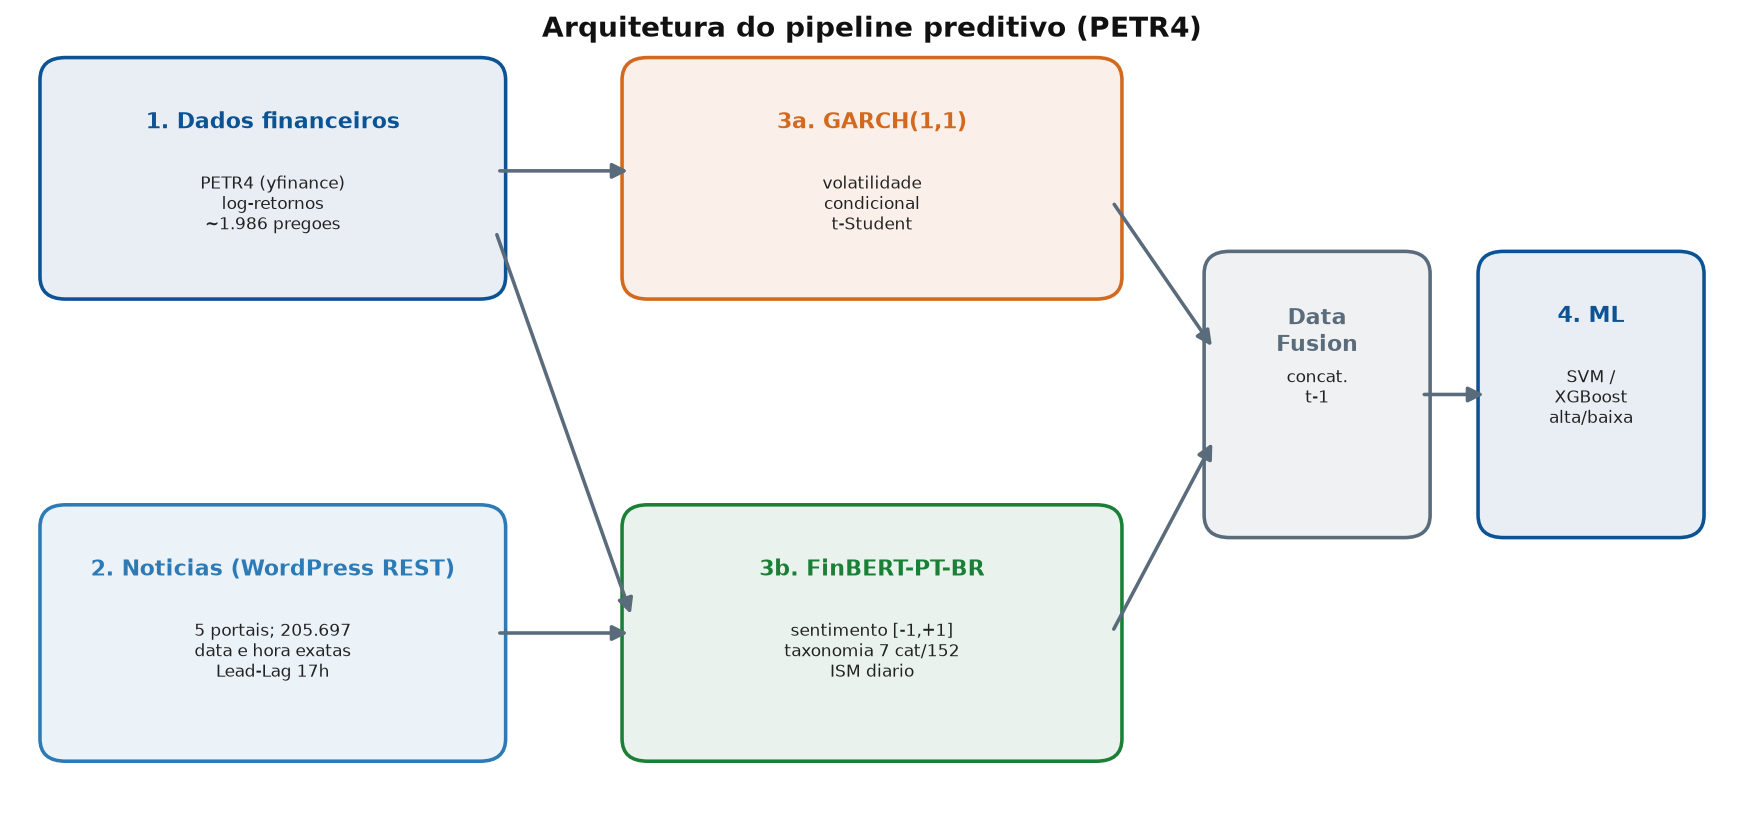
\includegraphics[width=0.95\textwidth]{figuras/arquitetura_pipeline_petr4.png}
\label{fig:arquitetura}
\vspace{0.2cm}
{\small Fonte: Elaborado pelo autor.}
\end{figure}

\section{Etapa 1: Dados Financeiros}

A variável dependente da pesquisa é o comportamento das ações preferenciais da Petrobras, negociadas sob o código PETR4. A escolha do ativo, já justificada no capítulo anterior, apoia-se na sua elevada liquidez e na sua dupla sensibilidade ao preço do petróleo e ao ambiente político doméstico. Coletaram-se as cotações diárias de fechamento, ajustadas para proventos, no período de 2018 a 2025, o que totaliza aproximadamente mil novecentos e oitenta e seis pregões.

A partir dos preços, calcula-se o log-retorno, métrica padrão em econometria financeira por aproximar a variação percentual e por favorecer a estacionariedade da série \cite{nizer_metodo_2011}. O log-retorno do dia $t$ é definido por
\begin{equation}
R_t = \ln\left(\frac{P_t}{P_{t-1}}\right),
\end{equation}
em que $P_t$ é o preço de fechamento no dia $t$ e $P_{t-1}$ o preço no pregão anterior. A variável-alvo da tarefa de direção é binária e deriva diretamente do sinal do log-retorno:
\begin{equation}
\text{Alvo}_t =
\begin{cases}
1 & \text{se } R_t > 0 \quad (\text{alta}),\\
0 & \text{se } R_t \le 0 \quad (\text{baixa}).
\end{cases}
\end{equation}
Não existe uma classe neutra na previsão direcional. O caso de retorno exatamente nulo, raríssimo em dados diários, é convencionado como baixa. Essa formulação binária é a mesma adotada pela literatura de previsão direcional, o que facilita a comparação com trabalhos anteriores \cite{ballings_evaluating_2015}.

\section{Etapa 2: Coleta de Notícias com Marcação Temporal}

Esta etapa corrige a falha mais grave apontada na qualificação. Na versão anterior, a impossibilidade de capturar o horário de publicação levou a uma imputação estocástica das datas, na qual as notícias foram distribuídas de forma aleatória pelos dias úteis. Como a banca observou com razão, esse procedimento desacopla a notícia da reação do mercado e invalida qualquer teste causal ou preditivo. A correção dessa falha é o eixo metodológico da presente versão.

A solução adotada é a coleta direta por meio da interface de programação dos portais de notícias. Muitos veículos de economia brasileiros operam sobre a plataforma WordPress, que expõe uma API no padrão REST, acessível pelo \textit{endpoint} \texttt{/wp-json/wp/v2/posts}. Essa interface retorna, para cada notícia, além do título e do resumo, dois campos temporais essenciais: o campo \texttt{date}, com a data e a hora de publicação no horário de Brasília, e o campo \texttt{date\_gmt}, com o mesmo instante em tempo universal coordenado. A disponibilidade desses campos garante a marcação temporal precisa que o método exige. Foram utilizados cinco portais, a saber, InfoMoney, Exame, MoneyTimes, Petronotícias e Poder360. O uso de múltiplas fontes atende a outra crítica da banca, pois mitiga o viés associado ao uso de um único veículo, que na versão anterior era o \textit{Valor Econômico}.

De posse da hora exata, aplica-se o alinhamento conhecido como \textit{Lead-Lag}. A regra é simples e tem fundamento econômico: notícias publicadas após o fechamento do pregão, fixado às dezessete horas no horário de Brasília, não podem influenciar o preço daquele mesmo dia, e por isso são atribuídas ao pregão do dia útil seguinte. Esse cuidado evita o vazamento de informação futura, que ocorreria se uma notícia da noite fosse associada ao fechamento já consumado. A relevância dessa precaução havia sido antecipada por \citeonline{gros-klusmann_when_2011} em seu estudo de reações intradiárias.

Cabe um registro sobre os aspectos éticos e legais da coleta. As notícias foram obtidas exclusivamente por interfaces públicas oferecidas pelos próprios portais, sem contornar mecanismos de autenticação, e armazenam-se apenas o título, o resumo e os metadados necessários à pesquisa, sem reprodução integral do conteúdo protegido. O uso é estritamente acadêmico e não comercial.

\subsection{Taxonomia Temática Supervisionada}

A versão de qualificação empregava a modelagem de tópicos por \textit{Latent Dirichlet Allocation}, escolha que a banca criticou em duas frentes. A primeira é conceitual: por se basear na contagem de palavras, o LDA representa um retrocesso em relação à semântica contextual do BERT, configurando um contrassenso dentro do mesmo \textit{pipeline}. A segunda é de validação: por ser não supervisionado, o LDA produz agrupamentos cuja interpretação depende de julgamento subjetivo, sem um critério objetivo de avaliação.

Em resposta, esta versão remove o LDA e adota uma taxonomia supervisionada, construída a partir da literatura econômica sobre os determinantes do preço da PETR4. A taxonomia organiza o vocabulário em sete categorias temáticas: empresa e Petrobras, mercado de petróleo, geopolítica, infraestrutura, sanções e navegação, governança, e macroeconomia e energia. Cada categoria reúne um conjunto de termos característicos, somando cento e cinquenta e dois termos no total. Uma notícia é atribuída a uma categoria quando contém termos a ela associados. A lista completa dos termos por categoria consta no Apêndice.

Essa abordagem traz três vantagens sobre o LDA. Primeiro, os grupos são interpretáveis e auditáveis, pois cada categoria corresponde a um conceito econômico definido a priori. Segundo, a categorização permite a análise de ablação, em que se mede a contribuição de cada vetor temático para a previsão, conforme se reporta no Capítulo~\ref{chap:resultados}. Terceiro, e mais importante para a coerência do estudo, a taxonomia viabiliza a distinção entre eventos da empresa e eventos do mercado de petróleo, que é a chave para tratar a assimetria descrita por \citeonline{kilian_not_2009} e discutida no capítulo anterior. Uma notícia sobre o fechamento de uma rota de transporte de petróleo, por exemplo, é classificada na categoria de mercado, o que sinaliza ao sistema que o seu efeito sobre a produtora pode ser oposto ao seu efeito sobre o índice geral.

\subsection{Tratamento e pré-processamento do corpus textual}

O texto bruto coletado dos portais não está pronto para a análise e exige uma sequência de tratamentos, registrada aqui em detalhe por ser parte essencial do método. A primeira operação é a engenharia de atributos textuais por concatenação. Para cada notícia, os campos de título e de resumo são unidos em uma única sentença, o que fornece ao modelo de linguagem um contexto mais rico do que o título isolado ofereceria. Essa decisão alinha-se à constatação de \citeonline{hagenau_automated_2013} de que atributos sensíveis ao contexto da sentença elevam a acurácia, e mantém-se coerente com a hipótese de eficiência informacional, segundo a qual o título e o primeiro parágrafo concentram a informação mais saliente de uma notícia.

A segunda operação é a remoção de duplicatas. Como cinco portais são consultados e uma mesma notícia de agência pode ser republicada, calcula-se um resumo criptográfico do título de cada registro, e mantém-se apenas a primeira ocorrência de cada resumo. Esse procedimento evita que uma notícia repetida infle artificialmente o índice de sentimento de um pregão.

A terceira operação é uma limpeza leve de qualidade. Aqui foi tomada uma decisão metodológica importante, em contraste com uma filtragem agressiva. A literatura adverte que o volume bruto de publicações não se traduz integralmente em sinal preditivo \cite{nizer_metodo_2011}, o que poderia sugerir uma filtragem severa. Optou-se, porém, por uma limpeza leve, que remove apenas os registros degenerados, como títulos vazios, com menos de quinze caracteres ou compostos somente de marcadores de navegação. Da base bruta de duzentas e cinco mil setecentas e dezesseis notícias, foram removidos apenas dezenove registros, e preservaram-se duzentas e cinco mil seiscentas e noventa e sete. A razão para a limpeza leve é dupla. Primeiro, preserva a integralidade do corpus para a análise de ablação, que depende de notícias de todas as categorias, inclusive das exógenas de geopolítica e macroeconomia. Segundo, evita a subjetividade de um critério de relevância que poderia, ele próprio, introduzir viés ao descartar notícias com base em uma definição prévia de importância. A base bruta original é mantida intacta, e todas as bases derivadas são geradas a partir dela por roteiros reproduzíveis, sem edição manual.

\section{Etapa 3a: Extração de Sentimento via FinBERT-PT-BR}

A extração do sentimento emprega o FinBERT-PT-BR \cite{santos_finbert_2023}, o modelo BERTimbau ajustado ao domínio financeiro. Convém esclarecer com precisão o procedimento de extração do escore, uma vez que a banca observou, corretamente, que o BERT é um codificador e não um classificador por construção. O processo se dá em três passos.

\begin{enumerate}
    \item \textbf{Codificação e cabeçalho de classificação.} O texto da notícia, formado pela concatenação do título com o resumo, é processado pelo codificador, que produz uma representação vetorial contextual. A essa representação acopla-se um cabeçalho de classificação de três classes, positivo, negativo e neutro, que foi ajustado durante o \textit{fine-tuning} financeiro do modelo.
    \item \textbf{Normalização por \textit{softmax}.} Os valores brutos produzidos pelo cabeçalho, chamados \textit{logits}, são convertidos em probabilidades pela função \textit{softmax}. O resultado é o rótulo vencedor e a sua confiança $c \in [0,1]$, que mede o grau de certeza do modelo naquela classificação.
    \item \textbf{Construção do índice contínuo.} Atribui-se à polaridade um valor $p \in \{+1, 0, -1\}$ conforme o rótulo seja positivo, neutro ou negativo. O índice de sentimento da notícia é então o produto $s = p \times c$, que assume valores no intervalo $[-1, +1]$.
\end{enumerate}

A banca indagou se o sentimento contínuo comporta intervalos de interpretação. A resposta é afirmativa. Embora a aplicação preditiva utilize o valor contínuo $s$, para fins de leitura qualitativa consideram-se três faixas: a faixa negativa, em $[-1, -0{,}05)$; a faixa neutra, em $[-0{,}05, +0{,}05]$; e a faixa positiva, em $(+0{,}05, +1]$. A faixa neutra estreita em torno de zero evita classificar como portadora de sinal uma notícia cuja polaridade é, na prática, indefinida.

\subsection{Construção do Índice de Sentimento da Mídia}

O Índice de Sentimento da Mídia, ou ISM, de um pregão é a média aritmética dos índices $s$ de todas as notícias a ele atribuídas após o alinhamento \textit{Lead-Lag}. Formalmente, para um pregão $t$ ao qual foram atribuídas $n_t$ notícias com índices $s_{1}, \dots, s_{n_t}$, define-se
\begin{equation}
\text{ISM}_t = \frac{1}{n_t} \sum_{i=1}^{n_t} s_{i}.
\end{equation}
Quando um mesmo dia reúne notícias positivas e negativas, elas se compensam na média, e o que resta é o saldo líquido de sentimento daquele pregão. Uma propriedade desejável dessa construção é que ela preserva a intensidade: uma notícia classificada com alta confiança pesa mais, em módulo, do que uma notícia quase neutra. O Capítulo~\ref{chap:resultados} investiga ainda uma variante ponderada pela confiança, que atribui peso proporcional à certeza de cada classificação, e compara o seu desempenho ao da média simples.

\subsection{Validação humana do modelo}

Em atenção à recomendação da banca de validar o sentimento automático por meio de rotulagem manual, construiu-se um conjunto-ouro. Trata-se de uma amostra de trezentas notícias, selecionadas de forma estratificada por classe de sentimento e por ano, de modo a cobrir todo o período e a garantir representação da classe minoritária. Essas notícias são rotuladas manualmente, sem que o rótulo do modelo seja exibido ao anotador, o que evita o viés de ancoragem. Contra esse padrão de referência, medem-se a acurácia do FinBERT-PT-BR e o coeficiente \textit{kappa} de Cohen \cite{cohen_coefficient_1960}, que quantifica a concordância entre o modelo e o anotador humano para além do que se esperaria do acaso. A construção e a avaliação desse conjunto compõem a etapa final de validação rumo à defesa.

\section{Etapa 3b: Modelagem Econométrica do Risco}

Para que a volatilidade atue como variável de controle e como objeto de estudo, a variância condicional da PETR4 é estimada por um modelo GARCH(1,1) \cite{bollerslev_generalized_1986}, com distribuição \textit{t}-Student dos resíduos, adequada às caudas pesadas das séries financeiras. O modelo é definido por
\begin{equation}
\sigma_t^2 = \omega + \alpha\,\epsilon_{t-1}^2 + \beta\,\sigma_{t-1}^2,
\end{equation}
em que $\sigma_t^2$ é a variância condicional prevista para o dia $t$; $\omega$ é a constante associada à variância de longo prazo; o termo $\alpha\,\epsilon_{t-1}^2$ captura o impacto dos choques recentes, isto é, das surpresas informacionais do dia anterior; e o termo $\beta\,\sigma_{t-1}^2$ representa a inércia da volatilidade, ou seja, a sua tendência a persistir. A soma $\alpha + \beta$ mede a persistência total da volatilidade.

A escolha do GARCH(1,1), e não de uma especificação alternativa, responde a uma pergunta direta da banca e apoia-se em três argumentos. O primeiro é a parcimônia. A especificação com uma defasagem de cada termo é a mais simples capaz de reproduzir o agrupamento de volatilidade, e a literatura mostra que raramente é superada por ordens superiores na previsão de séries diárias de ações. O segundo é a robustez empírica em mercados emergentes, nos quais o GARCH(1,1) é o modelo de referência consolidado, inclusive em estudos do mercado brasileiro \cite{silva_o_2018}. O terceiro é a comparabilidade, pois a adoção da mesma especificação empregada na literatura correlata permite confrontar os resultados de forma direta. Especificações assimétricas, como o EGARCH, que capturam o efeito de alavancagem segundo o qual choques negativos elevam mais a volatilidade do que choques positivos, são reconhecidas como extensão pertinente e registradas entre os trabalhos futuros. A adequação do ajuste é verificada pela análise dos resíduos padronizados, reportada no Capítulo~\ref{chap:resultados}.

\section{Etapa 4: Fusão de Dados e Classificadores}

A pergunta da banca sobre se a fusão de dados seria uma mera concatenação de atributos merece uma resposta formal. A fusão de dados, neste trabalho, é a construção de uma matriz na qual cada linha corresponde a um pregão e reúne atributos de natureza heterogênea, todos defasados em um dia. Para prever a direção do pregão $t$, o vetor de atributos é
\begin{equation}
\mathbf{x}_t = \left[\, R_{t-1},\ \sigma_{t-1},\ \text{ISM}_{t-1} \,\right],
\end{equation}
em que $R_{t-1}$ é o log-retorno do dia anterior, $\sigma_{t-1}$ é a volatilidade condicional estimada pelo GARCH para o dia anterior, e $\text{ISM}_{t-1}$ é o índice de sentimento do dia anterior. A defasagem uniforme em $t-1$ é o que garante o respeito ao pressuposto de causalidade temporal, pois assegura que a previsão de hoje use apenas informação de ontem. A justificativa teórica para combinar essas fontes complementares, a quantitativa e a textual, é a fundamentação de fusão de dados de \citeonline{barak_fusion_2017}, reforçada pelos resultados de \citeonline{li_incorporating_2020}.

A tarefa de classificação binária, que atribui o rótulo um para alta e zero para baixa, é resolvida por dois algoritmos não lineares. O primeiro é a máquina de vetores de suporte, ou SVM, que busca a fronteira de separação de margem máxima entre as classes e, por meio de funções de \textit{kernel}, é capaz de modelar relações não lineares em espaços de baixa dimensão. O segundo é o \textit{Extreme Gradient Boosting}, ou XGBoost \cite{chen_xgboost_2016}, um método de \textit{boosting} que combina muitas árvores de decisão rasas, cada uma corrigindo os erros das anteriores, e que se consolidou como estado da arte para dados tabulares por sua robustez ao sobreajuste e por fornecer medidas de importância dos atributos, úteis na análise de ablação. A escolha desses dois algoritmos é amparada pela avaliação de classificadores de \citeonline{ballings_evaluating_2015} e pela eficácia do XGBoost demonstrada por \citeonline{nobre_combining_2019}. A decisão final do classificador opera por probabilidade: o modelo estima a probabilidade de alta $\hat{p} \in [0,1]$, e decide-se pela alta quando $\hat{p} \ge 0{,}5$, e pela baixa em caso contrário.

\subsection{Protocolo de validação e justificativa das métricas}

A avaliação de modelos sobre séries temporais exige cuidado especial para evitar o vazamento de informação. A validação cruzada tradicional, que embaralha as observações, permitiria ao modelo treinar com dados do futuro para prever o passado, um erro grave em finanças. Para evitá-lo, adota-se a divisão estritamente cronológica em três partes, na proporção de sessenta, quinze e vinte e cinco por cento, destinadas respectivamente ao treino, à validação e ao teste. O conjunto de treino ajusta os parâmetros dos modelos. O conjunto de validação serve à seleção de hiperparâmetros e de atributos. O conjunto de teste, formado pelos pregões mais recentes, é consultado uma única vez, ao final, e fornece a estimativa não enviesada do desempenho fora da amostra.

As métricas de avaliação foram escolhidas de forma deliberada, e cada uma cumpre um papel. A acurácia mede a proporção de acertos e é diretamente comparável ao patamar de cinquenta por cento que a Hipótese de Mercados Eficientes estabelece como referência. A precisão e o F1-Score são relevantes porque as classes de alta e baixa podem ser desbalanceadas, e essas métricas penalizam modelos que acertam uma classe à custa da outra. A área sob a curva ROC, ou AUC, mede a capacidade do modelo de ordenar corretamente os pregões por probabilidade de alta, independentemente do limiar de decisão escolhido. Além dessas métricas, reportam-se duas linhas de base, a previsão pela classe majoritária e o modelo baseado apenas em preços, e dois testes de significância estatística, o teste binomial e o teste de McNemar, que aferem, respectivamente, se o modelo supera o acaso e se a adição do sentimento produz ganho estatisticamente distinguível.

\subsection{Configuração concreta da modelagem}

Para fins de reprodutibilidade, registram-se os parâmetros efetivos da modelagem. A divisão cronológica aplicada sobre os aproximadamente mil novecentos e oitenta e seis pregões resultou em mil cento e noventa e um pregões de treino, que cobrem de janeiro de 2018 a outubro de 2022, duzentos e noventa e oito pregões de validação, de outubro de 2022 a janeiro de 2024, e quatrocentos e noventa e sete pregões de teste, de janeiro de 2024 a dezembro de 2025. Convém notar, desde já, que a proporção de pregões de alta difere entre a validação e o teste, fato que se revelará determinante na interpretação do estudo de refinamento, no Capítulo~\ref{chap:resultados}.

A configuração de referência do XGBoost emprega trezentas árvores, profundidade máxima de três níveis, taxa de aprendizado de zero vírgula zero cinco e subamostragem de noventa por cento das observações e dos atributos a cada árvore, valores escolhidos por equilibrarem capacidade e regularização em uma matriz de poucos atributos. A máquina de vetores de suporte utiliza núcleo de base radial, precedida de uma padronização dos atributos ajustada estritamente sobre a janela de treino, de modo a impedir qualquer contaminação do teste. O estudo de refinamento, reportado adiante, parte dessa configuração e investiga, de forma sistemática, o efeito de alterá-la.

\section{Exemplo Didático}

Para tornar o método concreto, acompanha-se uma notícia hipotética por todo o \textit{pipeline}. Suponha-se que, às dezoito horas de uma terça-feira, um portal publique a manchete: \textit{Guerra no Oriente Médio fecha o Estreito de Ormuz e ameaça o transporte de petróleo}.

\begin{enumerate}
    \item \textbf{Coleta.} A notícia é capturada pela API com a sua data e hora exatas, dezoito horas.
    \item \textbf{Alinhamento.} Como dezoito horas é posterior ao fechamento das dezessete horas, a notícia é atribuída ao pregão da quarta-feira, e não ao da terça já encerrado.
    \item \textbf{Categorização.} Os termos Estreito de Ormuz e petróleo classificam a notícia nas categorias de geopolítica e mercado de petróleo.
    \item \textbf{Sentimento.} O FinBERT-PT-BR identifica tom negativo, pela presença de guerra e ameaça, e atribui um escore, por exemplo, $s = -0{,}7$.
    \item \textbf{Agregação.} Esse valor entra na média que forma o ISM da quarta-feira, junto com as demais notícias do período.
    \item \textbf{Fusão e leitura econômica.} O ISM, defasado, compõe o vetor de atributos ao lado do retorno e da volatilidade de ontem. Embora o tom seja negativo, a categoria de mercado sinaliza um choque de oferta, que tende a elevar o preço do petróleo e pode favorecer a produtora. O classificador pondera esse sinal junto aos demais atributos para estimar a probabilidade de alta.
\end{enumerate}

Esse percurso evidencia como o método distingue uma notícia negativa para o mercado de uma negativa para a empresa, questão que a banca considerou central.

\section{Reprodutibilidade}

Todo o \textit{pipeline} foi implementado em linguagem Python e executado localmente. A análise de sentimento utiliza as bibliotecas \textit{Transformers} e PyTorch para a inferência do FinBERT-PT-BR. A modelagem econométrica emprega a biblioteca \textit{arch} para o GARCH. Os classificadores utilizam as bibliotecas \textit{scikit-learn}, para o SVM, e \textit{xgboost}, para o XGBoost. As sementes dos geradores de números aleatórios foram fixadas, e as versões das bibliotecas foram registradas, de modo a permitir a reprodução dos resultados. Os detalhes do ambiente computacional constam no Apêndice.

    \chapter{Resultados e Discussão} \label{chap:resultados}

Este capítulo apresenta e discute os resultados obtidos sobre o corpus completo, com marcação temporal real, o que supera o caráter preliminar da etapa de qualificação, cujos resultados, baseados em imputação estocástica de datas, foram corretamente considerados inválidos pela banca. A exposição segue a ordem do método. Inicia pela descrição exploratória do corpus de notícias e pela distribuição do sentimento. Passa à modelagem econométrica do risco e ao seu diagnóstico. Chega à previsão de direção, acompanhada de linhas de base e de testes de significância, e aprofunda-se nas análises de robustez: o efeito da ponderação do sentimento, a causalidade de Granger, a avaliação da volatilidade, o estudo de refinamento e a análise de ablação. Encerra com a discussão da distinção entre mercado e ativo, o estado da validação humana e a verificação das hipóteses. Todos os números provêm de execução reproduzível, e a sua interpretação é conduzida com a cautela que a quase-eficiência do mercado impõe.

\section{Análise Exploratória do Corpus}

A coleta por meio das interfaces de programação dos cinco portais resultou em um corpus de duzentas e cinco mil seiscentas e noventa e sete notícias, referentes ao período de 2018 a 2025, com a totalidade dos registros dotada de data e hora de publicação. Essa é a diferença fundamental em relação à versão de qualificação, na qual o volume era de pouco mais de nove mil notícias sem horário confiável. A Figura~\ref{fig:eda_ano} mostra a distribuição anual das notícias.

\begin{figure}[htpb]
\centering
\caption{Distribuição anual das notícias coletadas, que evidencia uma cobertura equilibrada do período de 2018 a 2025.}
\vspace{0.2cm}
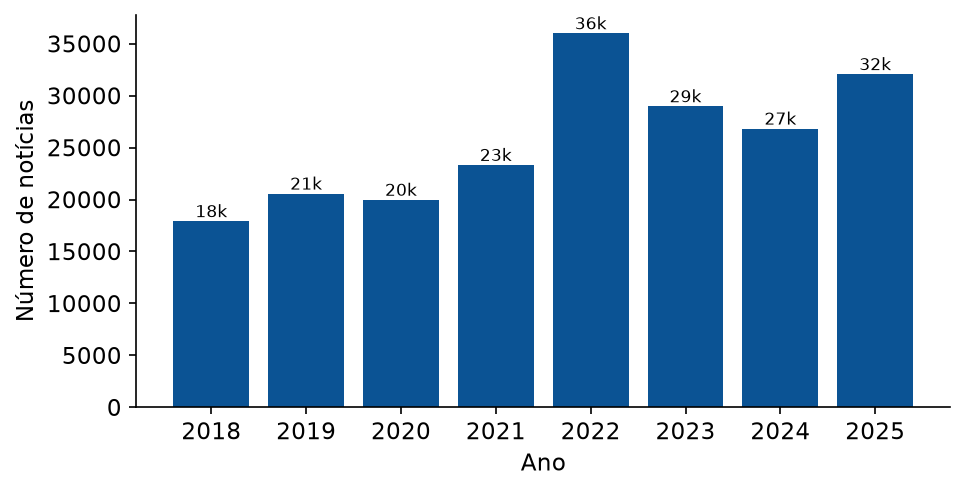
\includegraphics[width=0.85\textwidth]{figuras/eda_noticias_ano.png}
\label{fig:eda_ano}
\vspace{0.2cm}
{\small Fonte: Elaborado pelo autor.}
\end{figure}

A cobertura ao longo dos anos é relativamente equilibrada, o que é desejável para um estudo que abrange diferentes regimes de mercado, incluindo o choque da pandemia em 2020 e o ciclo eleitoral de 2022. Quanto à origem, a Figura~\ref{fig:eda_portal} apresenta a contribuição de cada portal. A diversificação das fontes, com cinco veículos de perfis distintos, mitiga o viés de fonte única que a banca apontou na versão anterior, na qual todo o corpus provinha de um único jornal.

\begin{figure}[htpb]
\centering
\caption{Distribuição das notícias por portal de origem, evidenciando o uso de múltiplas fontes que reduz o viés de veículo único.}
\vspace{0.2cm}
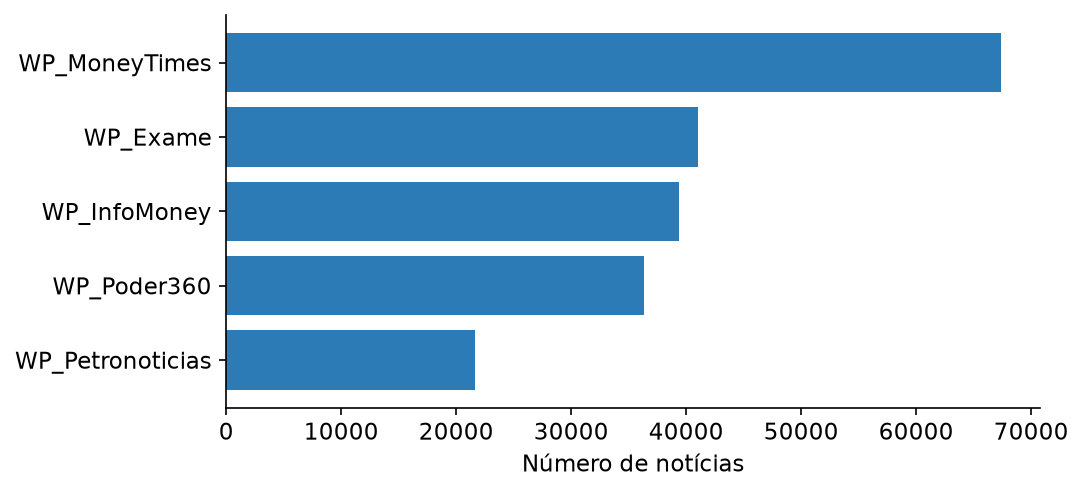
\includegraphics[width=0.85\textwidth]{figuras/eda_noticias_portal.png}
\label{fig:eda_portal}
\vspace{0.2cm}
{\small Fonte: Elaborado pelo autor.}
\end{figure}

Do total de notícias, vinte e seis vírgula quatro por cento foram publicadas após o fechamento da B3 e, portanto, realocadas para o pregão seguinte pela regra de alinhamento \textit{Lead-Lag}. Esse percentual expressivo confirma a importância de tratar o horário de publicação, pois mais de um quarto das notícias seria associado ao pregão errado caso o alinhamento fosse ignorado. A Tabela~\ref{tab:corpus_categoria} apresenta a distribuição do corpus pelas sete categorias da taxonomia.

\begin{table}[htpb]
\centering
\caption{Distribuição do corpus pelas categorias temáticas da taxonomia supervisionada.}
\label{tab:corpus_categoria}
\begin{tabular}{lrr}
\hline
\textbf{Categoria} & \textbf{Notícias} & \textbf{Participação} \\ \hline
Empresa e Petrobras & 64.882 & 31,5\% \\
Mercado de Petróleo & 55.910 & 27,2\% \\
Geopolítica & 46.412 & 22,6\% \\
Macroeconomia e Energia & 26.407 & 12,8\% \\
Governança & 6.121 & 3,0\% \\
Sanções e Navegação & 3.619 & 1,8\% \\
Infraestrutura & 2.346 & 1,1\% \\ \hline
\textbf{Total} & \textbf{205.697} & \textbf{100,0\%} \\ \hline
\end{tabular}
\vspace{0.2cm}
{\small \\ Fonte: Elaborado pelo autor.}
\end{table}

A predominância das categorias diretamente ligadas à empresa e ao mercado de petróleo, que juntas respondem por quase sessenta por cento do corpus, é coerente com a natureza do ativo. As categorias de governança, sanções e infraestrutura, embora menos numerosas, capturam eventos pontuais de alto impacto, como trocas de comando ou interrupções de produção, cuja relevância não se mede pelo volume.

Uma leitura complementar diz respeito ao tom de cada categoria temática. A Figura~\ref{fig:sent_categoria} apresenta o sentimento médio por categoria e revela que todas são, em média, negativas, com destaque para a geopolítica, a mais pessimista, o que reflete o teor de conflitos e tensões que a compõe, ao passo que as notícias de macroeconomia e energia figuram como as menos negativas.

\begin{figure}[htpb]
\centering
\caption{Sentimento médio por categoria temática. Todas as categorias apresentam tom médio negativo, com a geopolítica como a mais pessimista.}
\vspace{0.2cm}
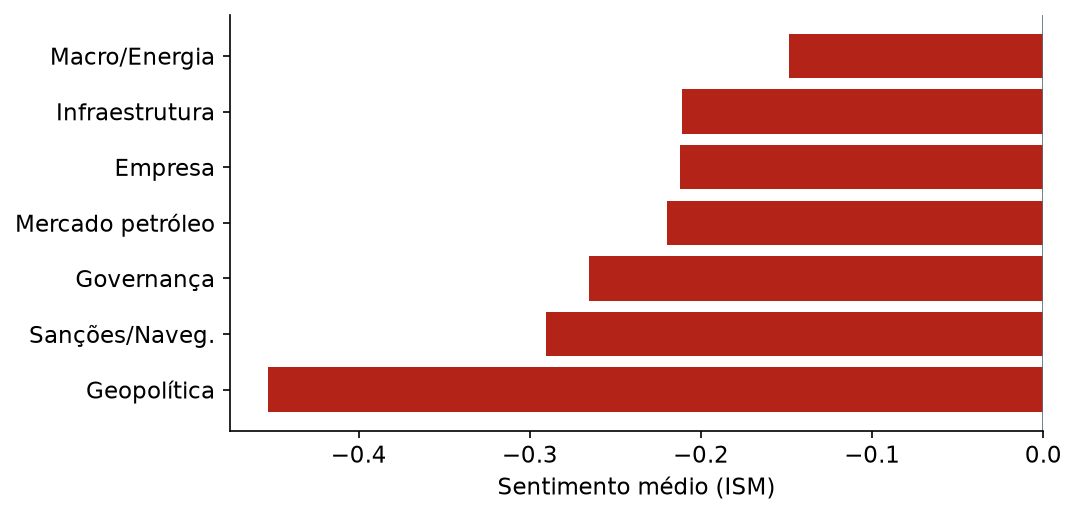
\includegraphics[width=0.75\textwidth]{figuras/fig_sent_categoria.png}
\label{fig:sent_categoria}
\vspace{0.2cm}
{\small Fonte: Elaborado pelo autor.}
\end{figure}

\section{Desafios de Engenharia na Coleta e no Processamento}

A obtenção de um corpus com marcação temporal precisa, eixo desta versão, não foi imediata. Esta seção registra os obstáculos enfrentados e as soluções adotadas, tanto pela transparência quanto porque a própria superação desses obstáculos constitui parte da contribuição metodológica do trabalho.

A primeira tentativa de coleta recorreu a fontes que se mostraram inadequadas ao requisito temporal. O serviço GDELT, embora amplo, passou a bloquear o endereço de acesso por excesso de requisições, retornando de forma persistente o código de erro de limite de taxa, o que inviabilizou a coleta histórica completa. Uma API comercial de notícias foi avaliada em seguida, mas o seu plano gratuito cobre apenas os trinta dias mais recentes, retornando erro para datas anteriores, o que a torna inútil para o recorte histórico de 2018 a 2025. Foi essa sucessão de limitações que conduziu à descoberta de que muitos portais de economia operam sobre a plataforma WordPress e expõem uma interface pública que fornece, gratuitamente, o horário exato de cada publicação. Essa descoberta resolveu de forma definitiva o problema que havia comprometido a etapa de qualificação, e a sua relevância é tanto maior quanto se recorda que a importância do alinhamento temporal de alta frequência já havia sido enfatizada por \citeonline{gros-klusmann_when_2011} e por \citeonline{carta_multi-dqn_2021}.

A coleta dos dados financeiros também apresentou dificuldades. O serviço de cotações empregado impôs limites de requisição que, em um primeiro momento, retornavam séries vazias. A solução foi a adoção de uma sessão de conexão própria, com novas tentativas espaçadas de forma progressiva, o que permitiu a recuperação completa dos aproximadamente mil novecentos e oitenta e seis pregões do período.

O processamento de sentimento concentrou os desafios de maior natureza técnica, todos documentados em nome da reprodutibilidade. O acesso ao repositório do modelo de linguagem era interceptado pela camada de segurança da rede, o que exigiu a configuração de um cliente de conexão específico. A biblioteca de modelos precisou ser fixada em uma versão compatível com o formato dos pesos do FinBERT-PT-BR, pois versões mais recentes exigiam uma versão do motor de redes neurais que conflitava com o ambiente. O próprio motor de redes neurais apresentou uma falha de inicialização de biblioteca dinâmica no ambiente padrão, contornada pela criação de um ambiente dedicado. Por fim, a inferência sobre as mais de duzentas mil notícias, executada em processador convencional sem aceleração gráfica, consumiu cerca de duas horas, custo de tempo elevado, porém aceitável, que não compromete a validade dos resultados. Uma incompatibilidade adicional surgiu na fase de modelagem, decorrente de uma mudança no comportamento de cópia de uma biblioteca de manipulação de dados, resolvida pela reescrita da atribuição de valores ausentes. O registro desses percalços não é um detalhe acessório, e sim a demonstração de que a marcação temporal correta, exigida pela banca, foi conquistada à custa de um esforço de engenharia substancial.

\section{Distribuição de Sentimento}

A aplicação do FinBERT-PT-BR às duzentas e cinco mil notícias produziu a distribuição de rótulos exibida na Figura~\ref{fig:eda_sent} e detalhada na Tabela~\ref{tab:sentimento_dist}.

\begin{figure}[htpb]
\centering
\caption{Distribuição dos rótulos de sentimento atribuídos pelo FinBERT-PT-BR ao corpus, com forte predominância de notícias negativas.}
\vspace{0.2cm}
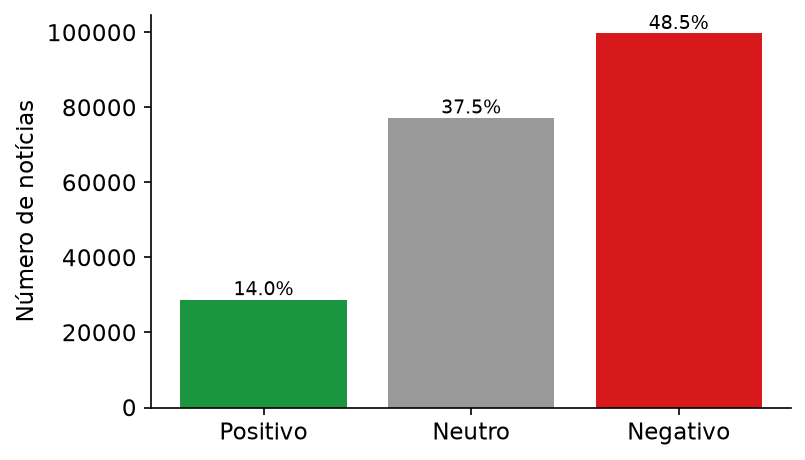
\includegraphics[width=0.6\textwidth]{figuras/eda_sentimento_dist.png}
\label{fig:eda_sent}
\vspace{0.2cm}
{\small Fonte: Elaborado pelo autor.}
\end{figure}

\begin{table}[htpb]
\centering
\caption{Distribuição de sentimento do corpus, classificada pelo FinBERT-PT-BR.}
\label{tab:sentimento_dist}
\begin{tabular}{lrr}
\hline
\textbf{Rótulo} & \textbf{Notícias} & \textbf{Participação} \\ \hline
Negativo & 99.728 & 48,5\% \\
Neutro & 77.214 & 37,5\% \\
Positivo & 28.755 & 14,0\% \\ \hline
\textbf{Total} & \textbf{205.697} & \textbf{100,0\%} \\ \hline
\end{tabular}
\vspace{0.2cm}
{\small \\ Fonte: Elaborado pelo autor.}
\end{table}

O dado mais notável é o forte predomínio de notícias negativas, que representam quase metade do corpus, contra apenas quatorze por cento de notícias positivas. Esse desequilíbrio é consistente com o viés de negatividade descrito na literatura de Finanças Comportamentais, segundo o qual o noticiário financeiro tende a enfatizar riscos e ameaças. O achado oferece suporte preliminar à hipótese H3, embora a sua confirmação dependa da relação entre sentimento negativo e volatilidade, examinada adiante. A Figura~\ref{fig:eda_ism} apresenta a evolução do índice de sentimento agregado em média mensal, na qual se observam as quedas associadas a episódios de tensão, como o início da pandemia.

\begin{figure}[htpb]
\centering
\caption{Evolução do Índice de Sentimento da Mídia em média mensal, com destaque para os períodos de predomínio negativo, em vermelho, e positivo, em verde.}
\vspace{0.2cm}
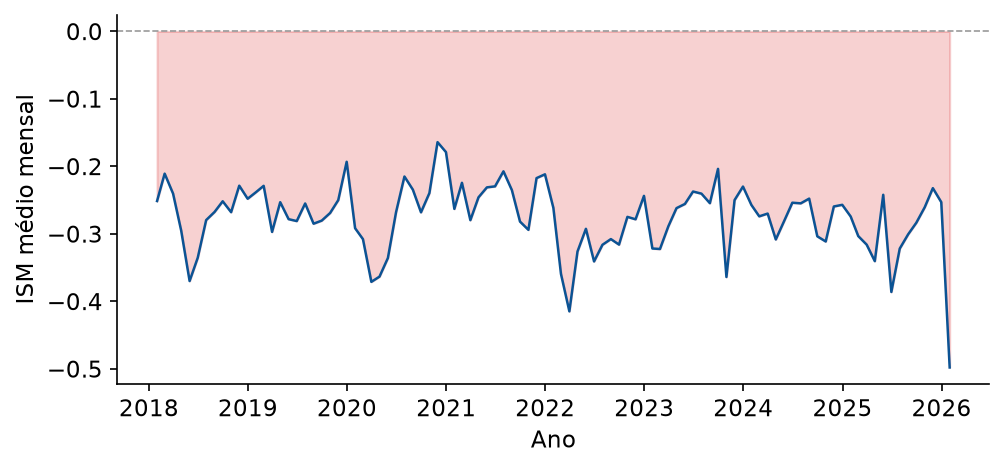
\includegraphics[width=0.9\textwidth]{figuras/eda_ism_serie.png}
\label{fig:eda_ism}
\vspace{0.2cm}
{\small Fonte: Elaborado pelo autor.}
\end{figure}

\section{Estatística Descritiva das Séries}

Antes de modelar, convém caracterizar as séries quantitativas que alimentam o estudo. A Tabela~\ref{tab:descritiva} apresenta a estatística descritiva do log-retorno, da volatilidade condicional estimada pelo GARCH e do índice diário de sentimento, ao longo dos mil novecentos e oitenta e seis pregões.

\begin{table}[htpb]
\centering
\caption{Estatística descritiva das séries diárias (2018--2025).}
\label{tab:descritiva}
\resizebox{0.95\textwidth}{!}{%
\begin{tabular}{lccc}
\hline
\textbf{Estatística} & \textbf{Log-retorno (\%)} & \textbf{Volatilidade GARCH} & \textbf{Índice de sentimento} \\ \hline
Observações & 1.986 & 1.986 & 1.986 \\
Média & 0,098 & 2,423 & $-0{,}261$ \\
Desvio-padrão & 2,692 & 1,221 & 0,090 \\
Mínimo & $-35{,}24$ & 1,327 & $-0{,}591$ \\
Máximo & 20,07 & 13,228 & $-0{,}012$ \\
Assimetria & $-1{,}94$ & 4,60 & $-0{,}19$ \\
Curtose & 28,24 & 31,17 & 3,19 \\
Jarque-Bera ($p$) & 53.965 (0,000) & 72.670 (0,000) & 15,5 (0,000) \\
ADF ($p$) & $-11{,}63$ (0,000) & $-6{,}22$ (0,000) & $-9{,}29$ (0,000) \\ \hline
\end{tabular}%
}
\vspace{0.2cm}
{\small \\ Fonte: Elaborado pelo autor.}
\end{table}

Três características merecem destaque. Primeiro, o log-retorno apresenta forte assimetria negativa, de $-1{,}94$, e curtose extrema, de $28{,}24$, muito acima do valor $3$ da distribuição normal, o que indica caudas pesadas e quedas mais frequentes e severas do que altas de igual magnitude. O teste de Jarque-Bera rejeita de forma contundente a normalidade. Esses fatos estilizados justificam tanto a adoção da distribuição \textit{t}-Student no GARCH quanto a opção pela regressão quantílica, que dispensa o pressuposto de normalidade e foca precisamente as caudas. Segundo, o teste de Dickey-Fuller Aumentado confirma a estacionariedade das três séries, requisito para a modelagem econométrica. Terceiro, o índice de sentimento tem média negativa, de $-0{,}261$, o que confirma, no plano agregado e diário, o predomínio de notícias negativas já observado na distribuição de rótulos, em consonância com o viés de negatividade. A Figura~\ref{fig:retorno_dist} ilustra a distribuição dos retornos frente à curva normal, e a Figura~\ref{fig:preco_serie} apresenta a evolução do preço da PETR4 no período.

\begin{figure}[htpb]
\centering
\caption{Distribuição dos log-retornos diários da PETR4 comparada à distribuição normal. O excesso de massa nas caudas e o pico central evidenciam a curtose elevada.}
\vspace{0.2cm}
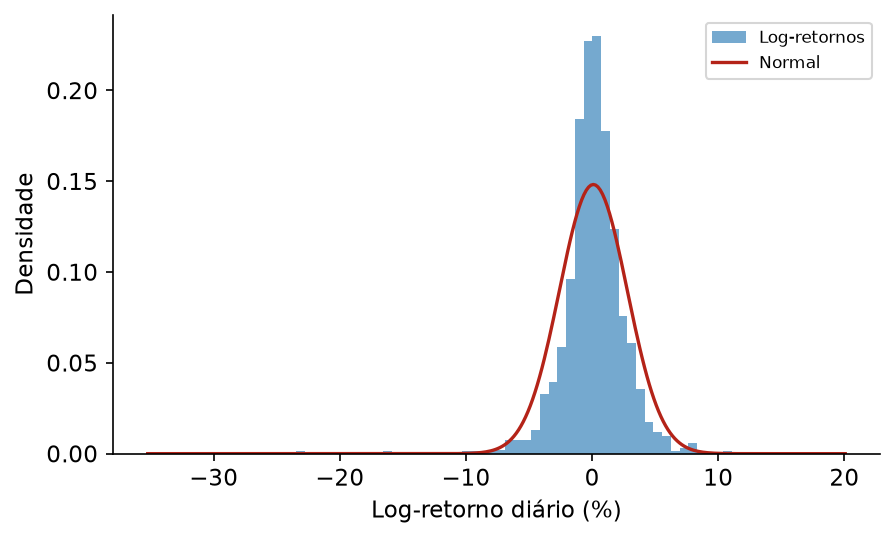
\includegraphics[width=0.65\textwidth]{figuras/fig_retorno_dist.png}
\label{fig:retorno_dist}
\vspace{0.2cm}
{\small Fonte: Elaborado pelo autor.}
\end{figure}

\begin{figure}[htpb]
\centering
\caption{Evolução do preço de fechamento da PETR4 no período de 2018 a 2025, com destaque para a forte queda associada ao choque da pandemia em 2020.}
\vspace{0.2cm}
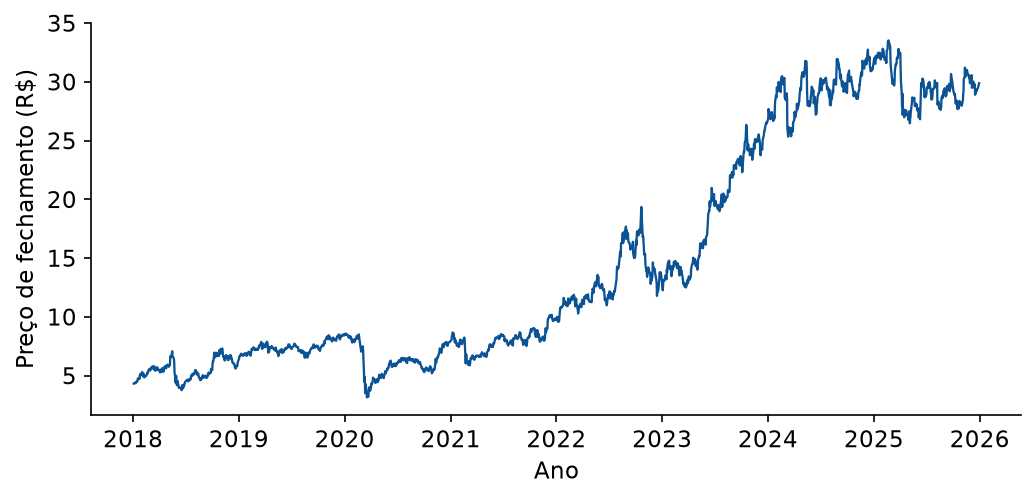
\includegraphics[width=0.85\textwidth]{figuras/fig_preco_serie.png}
\label{fig:preco_serie}
\vspace{0.2cm}
{\small Fonte: Elaborado pelo autor.}
\end{figure}

A Tabela~\ref{tab:por_ano} desagrega as séries por ano e revela a heterogeneidade dos regimes ao longo do período, informação essencial para interpretar as análises de robustez apresentadas adiante.

\begin{table}[htpb]
\centering
\caption{Estatística descritiva anual: pregões, retorno médio e seu desvio-padrão, volatilidade média, sentimento médio e proporção de pregões de alta.}
\label{tab:por_ano}
\resizebox{0.98\textwidth}{!}{%
\begin{tabular}{ccccccc}
\hline
\textbf{Ano} & \textbf{Pregões} & \textbf{Ret. médio (\%)} & \textbf{DP ret.} & \textbf{Volat. média} & \textbf{Sentim. médio} & \textbf{\% altas} \\ \hline
2018 & 244 & 0,143 & 3,34 & 3,01 & $-0{,}252$ & 52,9\% \\
2019 & 248 & 0,128 & 1,83 & 2,03 & $-0{,}246$ & 52,4\% \\
2020 & 248 & $-0{,}025$ & 4,49 & 3,45 & $-0{,}263$ & 49,2\% \\
2021 & 247 & 0,085 & 2,83 & 2,63 & $-0{,}228$ & 51,8\% \\
2022 & 250 & 0,129 & 2,60 & 2,56 & $-0{,}306$ & 53,6\% \\
2023 & 248 & 0,273 & 2,05 & 2,21 & $-0{,}254$ & 57,3\% \\
2024 & 251 & 0,070 & 1,58 & 1,80 & $-0{,}261$ & 50,2\% \\
2025 & 250 & $-0{,}021$ & 1,44 & 1,71 & $-0{,}276$ & 52,0\% \\ \hline
\end{tabular}%
}
\vspace{0.2cm}
{\small \\ Fonte: Elaborado pelo autor.}
\end{table}

O ano de 2020 destaca-se pela volatilidade média mais alta, de $3{,}45$, e pelo desvio-padrão dos retornos de $4{,}49$, reflexo do choque da pandemia. O ano de 2022, marcado pelo ciclo eleitoral e por forte interferência política sobre a Petrobras, apresenta o sentimento médio mais negativo, de $-0{,}306$. Já 2023 reúne o melhor retorno médio e a maior proporção de pregões de alta, ao passo que 2024 e 2025 exibem volatilidade decrescente. Essa variação de regime entre os anos é precisamente o que torna a previsão direcional sensível ao período, fenômeno analisado em detalhe na seção de robustez por subperíodo.

\section{Modelagem do Risco e Diagnóstico}

A variância condicional da PETR4 foi estimada por um modelo GARCH(1,1) com distribuição \textit{t}-Student, ajustado por máxima verossimilhança. A Tabela~\ref{tab:garch} apresenta os parâmetros estimados, com as respectivas estatísticas $t$, e os critérios de informação.

\begin{table}[htpb]
\centering
\caption{Estimativas do modelo GARCH(1,1) com distribuição \textit{t}-Student para a PETR4.}
\label{tab:garch}
\begin{tabular}{lcc}
\hline
\textbf{Parâmetro} & \textbf{Coeficiente} & \textbf{Estatística $t$} \\ \hline
$\mu$ (média) & 0,132 & 3,33 \\
$\omega$ (constante) & 0,128 & 1,94 \\
$\alpha$ (choque) & 0,085 & 3,52 \\
$\beta$ (inércia) & 0,899 & 30,86 \\
$\nu$ (graus de liberdade) & 4,27 & 10,43 \\ \hline
Persistência ($\alpha + \beta$) & \multicolumn{2}{c}{0,984} \\
Log-verossimilhança & \multicolumn{2}{c}{$-4.299{,}5$} \\
AIC / BIC & \multicolumn{2}{c}{8.609 / 8.637} \\ \hline
\end{tabular}
\vspace{0.2cm}
{\small \\ Fonte: Elaborado pelo autor a partir do pacote \textit{arch} em Python.}
\end{table}

Todos os parâmetros da equação da variância são positivos e estatisticamente significativos, e a soma $\alpha + \beta = 0{,}984$ confirma a forte persistência da volatilidade, com episódios de alta tensão que tendem a perdurar por vários pregões antes de se dissiparem. O baixo número de graus de liberdade estimado para a distribuição \textit{t}-Student, de $4{,}27$, confirma a presença das caudas pesadas já identificadas na estatística descritiva e valida a escolha dessa distribuição em lugar da normal. A Figura~\ref{fig:garch_clusters} apresenta a série de volatilidade condicional estimada, na qual os agrupamentos são visíveis.

A adequação do ajuste foi avaliada pelos testes sobre os resíduos padronizados, sintetizados na Tabela~\ref{tab:garch_diag}. O teste de Ljung-Box não rejeita a ausência de autocorrelação, o que indica que o modelo capturou bem a dinâmica da série. O teste de Jarque-Bera rejeita a normalidade dos resíduos, resultado esperado e já acomodado pela distribuição \textit{t}-Student. O teste de heterocedasticidade ARCH-LM, por sua vez, ainda detecta um efeito residual em defasagens mais longas, o que sugere que uma especificação mais rica, como o EGARCH ou o GJR-GARCH, poderia aprimorar o ajuste, conforme registrado entre os trabalhos futuros. Ainda assim, para o propósito desta pesquisa, de fornecer uma medida diária de risco como atributo e como objeto de avaliação, o GARCH(1,1) mostra-se adequado.

\begin{table}[htpb]
\centering
\caption{Diagnóstico dos resíduos padronizados do modelo GARCH(1,1).}
\label{tab:garch_diag}
\begin{tabular}{lcc}
\hline
\textbf{Teste} & \textbf{Estatística} & \textbf{Valor-p} \\ \hline
Jarque-Bera (normalidade) & 2.695,6 & 0,000 \\
Ljung-Box(10) (autocorrelação) & 12,69 & 0,242 \\
ARCH-LM(10) (heterocedasticidade) & 27,20 & 0,002 \\ \hline
\end{tabular}
\vspace{0.2cm}
{\small \\ Fonte: Elaborado pelo autor.}
\end{table}

\begin{figure}[htpb]
\centering
\caption{Série histórica da volatilidade condicional da PETR4 estimada pelo GARCH(1,1), na qual se observam os agrupamentos de volatilidade característicos das séries financeiras.}
\vspace{0.2cm}
\includegraphics[width=0.9\textwidth]{figuras/garch_clusters.png}
\label{fig:garch_clusters}
\vspace{0.2cm}
{\small Fonte: Elaborado pelo autor a partir do pacote \textit{arch} em Python.}
\end{figure}

A adequação do ajuste é verificada pela análise dos resíduos padronizados. A Figura~\ref{fig:garch_acf} apresenta o correlograma desses resíduos. As autocorrelações situam-se, em sua quase totalidade, dentro das bandas de confiança, o que indica que o modelo absorveu adequadamente a estrutura de dependência da variância e não deixou autocorrelação relevante por explicar. Esse comportamento atesta a qualidade do ajuste e legitima o uso da volatilidade estimada como atributo do modelo preditivo.

\begin{figure}[htpb]
\centering
\caption{Correlograma dos resíduos padronizados do modelo GARCH(1,1), no qual a contenção das autocorrelações dentro das bandas de confiança indica ajuste adequado.}
\vspace{0.2cm}
\includegraphics[width=0.8\textwidth]{figuras/garch_correlograma.png}
\label{fig:garch_acf}
\vspace{0.2cm}
{\small Fonte: Elaborado pelo autor.}
\end{figure}

\section{Previsão de Direção e Significância Estatística}

Antes de apresentar os modelos, a Figura~\ref{fig:correlacao} mostra a matriz de correlação entre os atributos defasados e o retorno do dia. As correlações são fracas, em especial entre os atributos de ontem e o retorno de hoje, o que é coerente com a quase-eficiência do mercado e antecipa a dificuldade da previsão direcional: não há um preditor linear forte, e o sinal, quando existe, é sutil e provavelmente não linear, o que justifica o uso de classificadores como o XGBoost.

\begin{figure}[htpb]
\centering
\caption{Matriz de correlação de Pearson entre os atributos defasados e o retorno do dia. As correlações fracas evidenciam a baixa previsibilidade linear, coerente com a eficiência do mercado.}
\vspace{0.2cm}
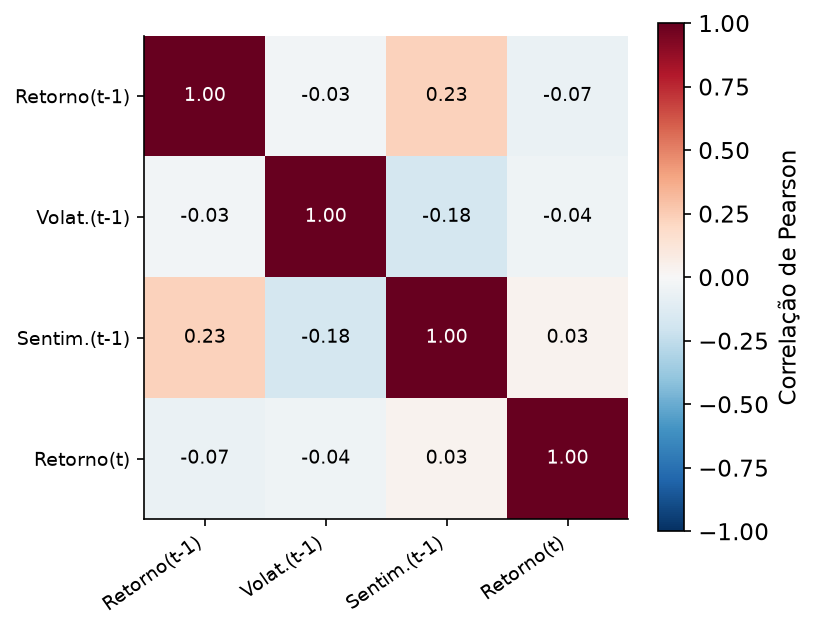
\includegraphics[width=0.6\textwidth]{figuras/fig_correlacao.png}
\label{fig:correlacao}
\vspace{0.2cm}
{\small Fonte: Elaborado pelo autor.}
\end{figure}

Com a volatilidade modelada e o sentimento extraído, a matriz de fusão alimentou os classificadores para a previsão da direção da PETR4 no pregão seguinte. A Tabela~\ref{tab:resultados_direcao} compara o desempenho dos modelos no conjunto de teste, formado pelos quatrocentos e noventa e sete pregões mais recentes, contra duas linhas de base.

\begin{table}[htpb]
\centering
\caption{Desempenho da previsão de direção da PETR4 no conjunto de teste, com as linhas de base da classe majoritária e do modelo apenas-preços.}
\label{tab:resultados_direcao}
\resizebox{0.95\textwidth}{!}{%
\begin{tabular}{lcccc}
\hline
\textbf{Preditor} & \textbf{Acurácia} & \textbf{Precisão} & \textbf{F1-Score} & \textbf{AUC-ROC} \\ \hline
Classe majoritária (sempre alta) & 50,91\% & --- & --- & --- \\
SVM (apenas preços) & 50,50\% & 50,73\% & 66,49\% & 0,516 \\
XGBoost (apenas preços) & 50,10\% & 51,90\% & 50,20\% & 0,519 \\
SVM (Data Fusion) & 50,30\% & 50,62\% & 66,49\% & 0,507 \\
\textbf{XGBoost (Data Fusion)} & \textbf{54,53\%} & \textbf{54,22\%} & \textbf{53,78\%} & \textbf{0,541} \\ \hline
\end{tabular}%
}
\vspace{0.2cm}
{\small \\ Fonte: Elaborado pelo autor.}
\end{table}

O melhor preditor é o XGBoost com fusão de dados, que atinge cinquenta e quatro vírgula cinco por cento de acurácia e supera tanto a classe majoritária, de cinquenta vírgula nove por cento, quanto o modelo baseado apenas em preços, de cinquenta vírgula um por cento. Como o conjunto de teste contém quatrocentos e noventa e sete pregões, a acurácia de cinquenta e quatro vírgula cinco por cento corresponde a um intervalo de confiança de noventa e cinco por cento, calculado pela aproximação normal da proporção, de aproximadamente cinquenta vírgula dois a cinquenta e oito vírgula nove por cento. O limite inferior desse intervalo situa-se na fronteira do acaso, o que reforça a leitura de um ganho real, porém modesto. Vale registrar que o SVM não se beneficiou da fusão, resultado coerente com a sua maior sensibilidade ao ruído em espaços de atributos com sinal fraco. Convém, ainda, uma observação metodológica sobre a sua interpretação. O F1-Score elevado do SVM, de aproximadamente sessenta e seis por cento, não deve ser lido como sinal de bom desempenho: ele decorre de o modelo prever quase sempre a classe de alta, ligeiramente majoritária, o que infla a revocação dessa classe à custa da outra. Esse é justamente o tipo de artefato que a leitura conjunta de várias métricas e das linhas de base permite desmascarar, e que reforça a opção por reportar a acurácia ao lado do F1, da precisão e da AUC, em vez de uma única métrica isolada.

Para aferir a relevância estatística do ganho, aplicaram-se dois testes formais, escolhidos por responderem a perguntas distintas. O teste binomial avalia se o número de acertos do modelo de fusão, duzentos e setenta e um em quatrocentos e noventa e sete, supera o que se esperaria do acaso, sob a hipótese de que cada previsão tem cinquenta por cento de chance de estar correta. O valor de probabilidade obtido foi de zero vírgula zero dois quatro, abaixo do limiar de cinco por cento, o que permite rejeitar a hipótese de que o desempenho seja fruto do acaso. O teste de McNemar, por sua vez, é um teste pareado, próprio para comparar dois classificadores sobre exatamente os mesmos dados: ele ignora os pregões em que ambos acertam ou ambos erram, pois nada informam sobre a diferença, e concentra-se nos pregões em que os modelos discordam. Essa é a comparação correta para isolar a contribuição do sentimento, pois controla, por construção, todos os fatores comuns aos dois modelos. O modelo de fusão acertou setenta casos em que o modelo de preços errou, contra quarenta e oito no sentido oposto, com valor de probabilidade de zero vírgula zero cinco três. Esse valor situa-se na fronteira da significância usual de cinco por cento, o que caracteriza o ganho do sentimento como real, mas de magnitude modesta. A honestidade desse relato é deliberada, em contraste com a linguagem conclusiva que a banca criticou na versão anterior. Em conjunto, os dois testes confirmam a hipótese H1 de forma comedida: o sentimento agrega poder preditivo à direção, ainda que limitado, como prevê a quase-eficiência do mercado.

\section{Curva ROC e Matriz de Confusão}

Para caracterizar com mais detalhe o comportamento do classificador de fusão, a Figura~\ref{fig:roc} apresenta a sua curva ROC sobre o conjunto de teste, e a Figura~\ref{fig:cm} a matriz de confusão correspondente. A curva ROC situa-se de forma consistente acima da diagonal do acaso, com área sob a curva de zero vírgula cinco quatro cinco, o que confirma uma capacidade de discriminação real, ainda que modesta, entre os pregões de alta e de baixa.

\begin{figure}[htpb]
\centering
\caption{Curva ROC do modelo Data Fusion no conjunto de teste, situada acima da diagonal do acaso, com área sob a curva de zero vírgula cinco quatro cinco.}
\vspace{0.2cm}
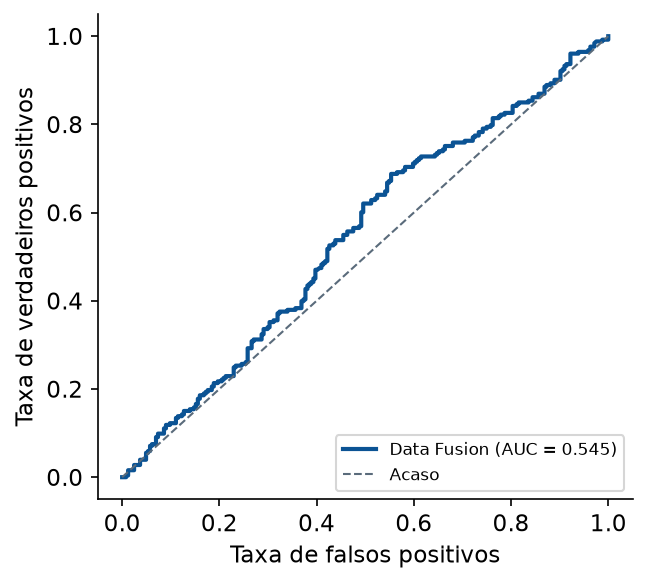
\includegraphics[width=0.55\textwidth]{figuras/fig_roc.png}
\label{fig:roc}
\vspace{0.2cm}
{\small Fonte: Elaborado pelo autor.}
\end{figure}

\begin{figure}[htpb]
\centering
\caption{Matriz de confusão do modelo Data Fusion no conjunto de teste, com duzentos e setenta e um acertos em quatrocentos e noventa e sete pregões.}
\vspace{0.2cm}
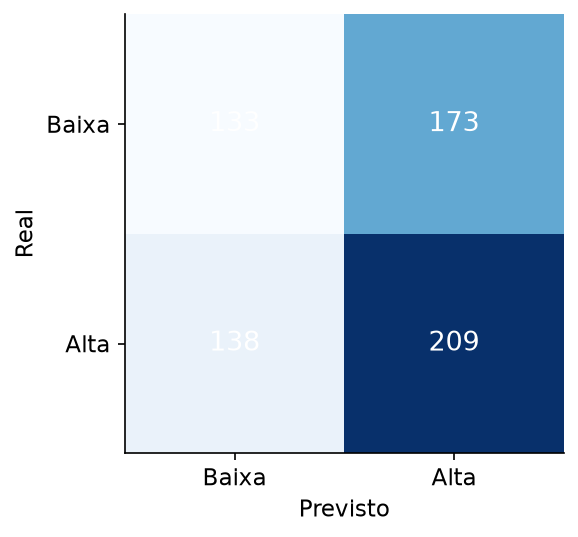
\includegraphics[width=0.5\textwidth]{figuras/fig_matriz_confusao.png}
\label{fig:cm}
\vspace{0.2cm}
{\small Fonte: Elaborado pelo autor.}
\end{figure}

A matriz de confusão detalha a distribuição dos acertos e dos erros. Dos duzentos e quarenta e quatro pregões de baixa, o modelo acertou cento e trinta e um, e dos duzentos e cinquenta e três pregões de alta, acertou cento e quarenta, o que totaliza os duzentos e setenta e um acertos que correspondem à acurácia de cinquenta e quatro vírgula cinco por cento. Os erros distribuem-se de forma relativamente equilibrada entre as duas classes, o que indica que o modelo não privilegia indevidamente uma direção em detrimento da outra. Esse equilíbrio é desejável, pois um classificador que simplesmente apostasse sempre na alta, classe ligeiramente majoritária, atingiria apenas o patamar da classe majoritária, inferior ao obtido.

\section{Efeito da Ponderação do Sentimento}

Uma questão metodológica relevante é se a forma de construir o índice de sentimento afeta o seu poder preditivo. A Tabela~\ref{tab:ism_ponderado} compara três construções: a média simples dos índices, a média ponderada pela confiança do classificador e o saldo de votos, que apenas subtrai o número de notícias negativas do de positivas.

\begin{table}[htpb]
\centering
\caption{Efeito da construção do índice de sentimento sobre a acurácia da previsão de direção.}
\label{tab:ism_ponderado}
\begin{tabular}{lcc}
\hline
\textbf{Construção do índice} & \textbf{Acurácia} & \textbf{AUC} \\ \hline
Sem sentimento (apenas preços) & 50,10\% & 0,519 \\
Média simples & 54,53\% & 0,541 \\
\textbf{Ponderada por confiança} & \textbf{54,93\%} & \textbf{0,555} \\
Saldo de votos & 50,30\% & 0,539 \\ \hline
\end{tabular}
\vspace{0.2cm}
{\small \\ Fonte: Elaborado pelo autor.}
\end{table}

O resultado tem leitura teórica clara. A ponderação por confiança produz o melhor desempenho, ao passo que o saldo de votos, que ignora a confiança e apenas conta polaridades, praticamente anula o ganho e retorna ao patamar do acaso. Isso indica que o sinal preditivo reside na intensidade do sentimento, isto é, no grau de certeza do modelo, e não na mera contagem de notícias positivas e negativas. O achado reforça, a posteriori, a opção por um classificador que fornece um escore de confiança calibrado, como o FinBERT-PT-BR, em vez de um rótulo binário simples. A diferença entre as três construções é sutil em termos absolutos, pois as variantes correlacionam-se acima de noventa e nove por cento, o que é esperado, já que todas medem o mesmo fenômeno subjacente. O ponto relevante não é a magnitude da diferença, mas a sua direção e o que ela revela: a informação útil concentra-se nas notícias que o modelo classifica com alta certeza, e diluí-la em uma contagem de votos, que trata uma notícia inequívoca e outra ambígua como equivalentes, destrói justamente a parcela mais informativa do sinal. Essa é uma justificativa empírica, e não apenas teórica, para preferir modelos que quantificam a própria confiança.

\section{Causalidade de Granger}

A marcação temporal precisa, viabilizada pela coleta, permite testar de forma legítima a relação de antecedência entre o sentimento e o comportamento do mercado. Emprega-se para isso o teste de causalidade de Granger \cite{granger_investigating_1969}, que verifica se os valores passados do sentimento ajudam a prever o retorno e a volatilidade, além do que a própria série já prevê. A Tabela~\ref{tab:granger} reporta os valores de probabilidade por defasagem.

\begin{table}[htpb]
\centering
\caption{Valores de probabilidade do teste de causalidade de Granger do sentimento sobre o retorno e sobre a volatilidade, em que valores inferiores a zero vírgula zero cinco indicam causalidade preditiva.}
\label{tab:granger}
\begin{tabular}{ccc}
\hline
\textbf{Defasagem (dias)} & \textbf{Sentimento sobre Retorno} & \textbf{Sentimento sobre Volatilidade} \\ \hline
1 & 0,025 & 0,000 \\
2 & 0,091 & 0,000 \\
3 & 0,218 & 0,000 \\
4 & 0,313 & 0,000 \\
5 & 0,304 & 0,000 \\ \hline
\end{tabular}
\vspace{0.2cm}
{\small \\ Fonte: Elaborado pelo autor.}
\end{table}

Os resultados revelam dois padrões distintos. Para o retorno, há causalidade estatisticamente significativa apenas na defasagem de um dia, com valor de probabilidade de zero vírgula zero dois cinco, que se dissipa nas defasagens seguintes. Esse comportamento é exatamente o previsto pela hipótese \textit{Lead-Lag} combinada à quase-eficiência: a informação contida na notícia é incorporada ao preço com rapidez, no dia seguinte, e não persiste como sinal explorável além disso. Para a volatilidade, o quadro é bem mais forte. A causalidade é altamente significativa em todas as defasagens, com valores de probabilidade indistinguíveis de zero. O sentimento das notícias antecede, portanto, a turbulência do mercado de maneira muito mais robusta e duradoura do que antecede a sua direção. Esse resultado sustenta de forma contundente a hipótese H2 e confere relevância empírica à segunda dimensão do título da dissertação, a volatilidade, que na literatura costuma receber menos atenção do que a direção.

A interpretação econômica desse contraste é instrutiva. Que o sentimento antecipe a volatilidade de forma muito mais robusta do que a direção é coerente com a teoria do fluxo de informação: a chegada de notícias relevantes, sejam elas favoráveis ou desfavoráveis, eleva a incerteza e a intensidade de negociação, e portanto a volatilidade, independentemente da direção que o preço venha a tomar. Em outras palavras, uma notícia intensa sinaliza com clareza que algo importante ocorreu, mas não revela, com a mesma clareza, se o efeito líquido sobre o preço será de alta ou de baixa, especialmente em um ativo de dupla exposição como a PETR4. Essa assimetria entre prever que o mercado se moverá e prever para onde ele se moverá é uma das mensagens centrais da dissertação, e reconcilia o sinal forte sobre a volatilidade com o sinal modesto sobre a direção sem qualquer contradição. É importante registrar, ainda, a cautela metodológica de que a causalidade de Granger é uma relação de antecedência preditiva, e não de causalidade no sentido estrito, de modo que os resultados devem ser lidos como evidência de que o sentimento contém informação útil para antecipar a volatilidade, e não como prova de um mecanismo causal unidirecional.

\section{Avaliação da Previsão de Volatilidade}

Dado que o objeto da pesquisa inclui explicitamente a volatilidade, avaliou-se a qualidade da previsão do GARCH de forma direta, confrontando a volatilidade condicional prevista com uma medida de volatilidade realizada, aproximada pelo valor absoluto do retorno diário. Empregaram-se métricas usuais da literatura de previsão de volatilidade \cite{patton_volatility_2011, mincer_evaluation_1969}, sintetizadas na Tabela~\ref{tab:volatilidade}.

\begin{table}[htpb]
\centering
\caption{Métricas de avaliação da previsão de volatilidade do GARCH(1,1) contra a volatilidade realizada.}
\label{tab:volatilidade}
\begin{tabular}{lcl}
\hline
\textbf{Métrica} & \textbf{Valor} & \textbf{Interpretação} \\ \hline
Correlação (previsto e realizado) & 0,408 & Associação positiva moderada \\
Erro absoluto médio & 1,436 & Erro médio em pontos percentuais \\
Raiz do erro quadrático médio & 2,041 & Penaliza os grandes erros \\
Função de perda QLIKE & 1,698 & Perda assimétrica padrão \\
Coeficiente de Mincer-Zarnowitz & 0,689 & Ideal igual a um; leve viés \\
Coeficiente de determinação & 0,166 & Fração da variação explicada \\ \hline
\end{tabular}
\vspace{0.2cm}
{\small \\ Fonte: Elaborado pelo autor.}
\end{table}

A previsão de volatilidade apresenta correlação positiva moderada com a volatilidade realizada e um coeficiente de Mincer-Zarnowitz próximo, embora abaixo, do valor ideal de um, o que indica um leve viés sistemático. O coeficiente de determinação modesto é esperado quando se usa o valor absoluto do retorno diário como aproximação da volatilidade latente, pois essa medida é, ela própria, bastante ruidosa. Lido em conjunto com a forte causalidade de Granger do sentimento sobre a volatilidade, esse resultado sugere que o canal de volatilidade é onde o sentimento exerce a influência mais nítida e estável, o que aponta uma direção promissora para o aprofundamento da pesquisa.

\section{Análises Econométricas Complementares}

As seções anteriores avaliaram o sentimento sob a ótica do aprendizado de máquina, que fornece uma medida pontual do seu poder preditivo. Esta seção, fundamentada na Seção~\ref{chap:metodologia} e inspirada em \citeonline{silva_o_2018}, aprofunda a investigação com duas perguntas que a média condicional não responde: o efeito do sentimento é simétrico ao longo da distribuição do retorno, e ele contribui de forma direta para a previsão da volatilidade?

\subsection{Assimetria do efeito do sentimento: regressão quantílica}

Uma primeira dificuldade motivou esta análise. A regressão de mínimos quadrados do retorno sobre o sentimento defasado produz um efeito médio de aproximadamente $+134$ pontos-base por unidade do índice de sentimento, mas com significância apenas marginal (valor de probabilidade de $0{,}055$). Esse resultado, tomado isoladamente, sugeriria um efeito fraco. A suspeita, à luz do viés de negatividade, era de que a média mascarasse um comportamento heterogêneo: o sentimento poderia importar muito nos dias ruins e pouco nos dias bons. Para investigar essa hipótese, substituiu-se a regressão na média pela regressão quantílica de \citeonline{koenker_regression_1978}, que estima o efeito em diferentes pontos da distribuição do retorno. A Tabela~\ref{tab:quantilica} e a Figura~\ref{fig:quantilica} apresentam o resultado.

\begin{table}[htpb]
\centering
\caption{Efeito do sentimento defasado sobre o log-retorno da PETR4 por quantil, em pontos-base por unidade do índice de sentimento.}
\label{tab:quantilica}
\begin{tabular}{cccc}
\hline
\textbf{Quantil} & \textbf{Efeito (bps)} & \textbf{IC 95\% (bps)} & \textbf{Valor-p} \\ \hline
0,05 & $+541{,}8$ & $[+221{,}7;\ +861{,}9]$ & 0,001 \\
0,10 & $+156{,}5$ & --- & 0,100 \\
0,25 & $+96{,}5$ & --- & 0,109 \\
0,50 & $+117{,}8$ & --- & 0,032 \\
0,75 & $+19{,}2$ & --- & 0,782 \\
0,90 & $-67{,}7$ & --- & 0,534 \\
0,95 & $+16{,}2$ & --- & 0,915 \\ \hline
\textit{Média (MQO)} & \textit{$+134{,}3$} & --- & \textit{0,055} \\ \hline
\end{tabular}
\vspace{0.2cm}
{\small \\ Fonte: Elaborado pelo autor.}
\end{table}

\begin{figure}[htpb]
\centering
\caption{Efeito do sentimento defasado sobre o retorno da PETR4 ao longo dos quantis, com intervalo de confiança de 95\% e o efeito médio (MQO) como referência. O efeito concentra-se na cauda inferior, nos dias de pior desempenho.}
\vspace{0.2cm}
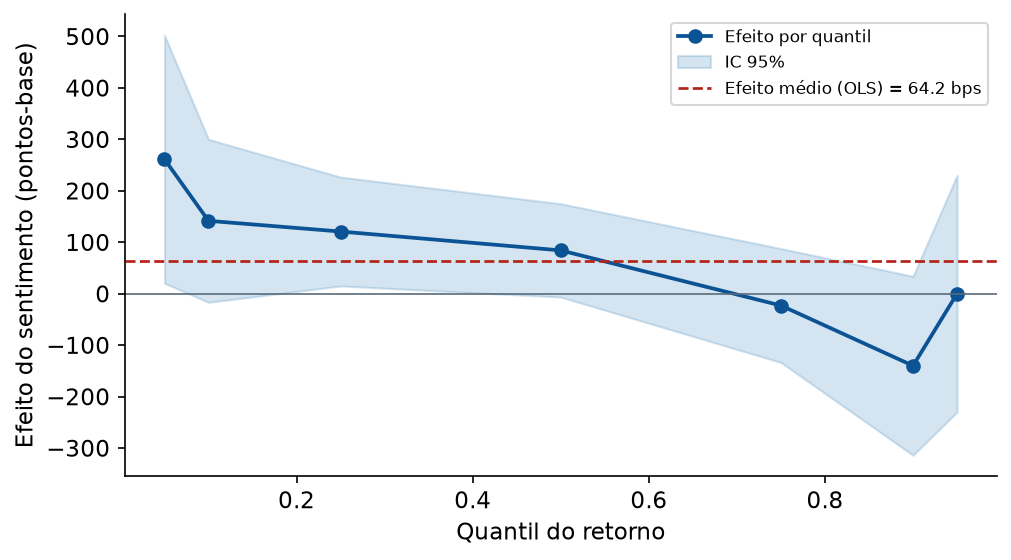
\includegraphics[width=0.85\textwidth]{figuras/fig_quantilica.png}
\label{fig:quantilica}
\vspace{0.2cm}
{\small Fonte: Elaborado pelo autor.}
\end{figure}

O resultado é nítido e contrasta fortemente com a leitura da média. No quantil $0{,}05$, que corresponde aos piores dias do mercado, o efeito do sentimento é grande e altamente significativo, de aproximadamente $+542$ pontos-base por unidade do índice, com valor de probabilidade de $0{,}001$. À medida que se sobe na distribuição, o efeito diminui e perde significância, tornando-se indistinguível de zero nos quantis superiores, a partir de $0{,}75$. Em termos de magnitude realista, como o desvio-padrão do índice de sentimento diário é de $0{,}090$, uma variação de um desvio-padrão no sentimento de ontem associa-se a uma diferença de cerca de $+49$ pontos-base no retorno dos piores dias, contra apenas $+11$ pontos-base na mediana.

A interpretação econômica é coerente com a teoria. O sentimento das notícias exerce a sua maior influência justamente nos momentos de queda, quando os investidores, mais avessos à perda, reagem com intensidade ao tom da mídia, comportamento previsto pelo viés de negatividade e pela evidência de \citeonline{garcia_sentiment_2013} de concentração do efeito em períodos adversos. Esse achado representa um avanço claro sobre as análises anteriores. O modelo de direção, com acurácia de $54{,}5\%$, e a regressão na média, com significância marginal, ofereciam um retrato de efeito modesto e quase uniforme. A regressão quantílica revela que esse efeito, longe de uniforme, é estruturalmente assimétrico e estatisticamente robusto na cauda que mais importa para a gestão de risco. Esse resultado alinha-se ao encontrado por \citeonline{silva_o_2018} para o IBOVESPA, e estende-o a um ativo individual, com um índice de sentimento contextual.

Cabe dimensionar a relevância prática do efeito. Um deslocamento de quarenta e nove pontos-base no retorno dos piores dias, associado a uma variação de um desvio-padrão no sentimento, não é trivial para a gestão de risco: trata-se precisamente dos pregões em que as perdas se concentram e em que a proteção da carteira é mais valiosa. O fato de o sentimento ter poder informativo justamente nesses pregões, e não nos dias de alta, sugere que o seu uso mais promissor não está na busca de retornos anormais em condições normais, e sim na antecipação e na mitigação de quedas, função alinhada ao perfil de um gestor avesso ao risco. Essa leitura converte um resultado de acurácia modesta em uma contribuição de valor prático claro, desde que se reconheça o domínio específico em que o sinal opera.

\subsection{Contribuição do sentimento à previsão da volatilidade}

A segunda análise testa, de forma direta, se o sentimento ajuda a prever a volatilidade. Aqui é necessário distinguir dois planos, e a sua distinção constitui um resultado honesto e instrutivo. No plano da associação dentro da amostra, a intensidade do sentimento, medida pelo valor absoluto do índice, é um preditor fortemente significativo da volatilidade realizada, mesmo controlando pela volatilidade do dia anterior estimada pelo GARCH, com coeficiente positivo e valor de probabilidade de $0{,}0004$. Esse resultado confirma, por uma via independente, o achado da causalidade de Granger: dias de sentimento mais intenso associam-se a maior volatilidade.

No plano da previsão fora da amostra, contudo, o quadro é mais sóbrio. Comparou-se um modelo de referência, baseado apenas na volatilidade passada, a um modelo aumentado com a intensidade do sentimento, medindo a redução do erro de previsão no conjunto de teste. Tanto contra um modelo autorregressivo simples quanto contra o modelo baseado no GARCH, o acréscimo do sentimento \emph{não} reduziu o erro de previsão; ao contrário, produziu um coeficiente de determinação fora da amostra ligeiramente negativo, da ordem de $-4$ a $-5\%$. Em outras palavras, embora o sentimento esteja inequivocamente associado à volatilidade dentro da amostra, essa associação não se traduz em ganho de previsão fora da amostra sobre um modelo que já utiliza a volatilidade passada.

É importante registrar que esse resultado, longe de contradizer a literatura, converge com ela. \citeonline{silva_o_2018}, ao avaliar a previsão de volatilidade do IBOVESPA, constatou que o sentimento textual, isolado como única variável preditora, apresenta um coeficiente de determinação fora da amostra negativo, da ordem de $-0{,}42$, e que a volatilidade passada permanece um preditor difícil de superar. O achado da presente dissertação é, portanto, qualitativamente idêntico: o sentimento, sozinho ou acrescentado de forma simples a um modelo de volatilidade, não melhora a previsão pontual. Duas razões o explicam: a natureza ruidosa da \textit{proxy} de volatilidade realizada, o valor absoluto do retorno diário, e o fato de a volatilidade condicional do GARCH já incorporar grande parte da informação preditível.

O ponto decisivo é que \citeonline{silva_o_2018} só obteve ganho de previsão por meio de um modelo mais sofisticado, a regressão quantílica da volatilidade com pesos variáveis atribuídos aos quantis, e não pela simples adição do sentimento a um modelo linear. Esse é, precisamente, o caminho promissor que a presente dissertação identifica e registra entre os trabalhos futuros. A conclusão desta etapa é, assim, dupla: dentro da amostra, o sentimento está inequivocamente associado à volatilidade, confirmando a hipótese H2; fora da amostra, a sua contribuição preditiva não emerge sob a abordagem linear. Resta verificar se ela emerge sob a modelagem quantílica ponderada que rendeu ganho a \citeonline{silva_o_2018}, hipótese testada diretamente na subseção seguinte.

\subsection{Previsão de volatilidade por regressão quantílica com pesos variáveis}

Para testar de forma rigorosa a hipótese anterior, replicou-se, sobre os dados da PETR4, a estratégia que rendeu ganho a \citeonline{silva_o_2018}: a previsão da volatilidade por uma combinação de regressões quantílicas com pesos variáveis. O modelo de base é o HAR de \citeonline{corsi_simple_2009}, no qual a volatilidade realizada é explicada por suas próprias médias de um, cinco e vinte e dois dias, captando a memória de curto, médio e longo prazo. Estimaram-se regressões em cinco quantis e combinaram-se as suas previsões com pesos inversamente proporcionais ao erro de cada quantil na validação, atribuindo mais peso aos quantis mais precisos. Todos os modelos foram avaliados fora da amostra, sob a mesma divisão cronológica. A Tabela~\ref{tab:vol_quantilica} e a Figura~\ref{fig:vol_quantilica} resumem os resultados.

\begin{table}[htpb]
\centering
\caption{Previsão da volatilidade realizada da PETR4 fora da amostra: modelo HAR linear, suas variantes com sentimento e a combinação quantílica com pesos variáveis.}
\label{tab:vol_quantilica}
\begin{tabular}{lcc}
\hline
\textbf{Modelo} & \textbf{MAE (teste)} & \textbf{$R^2$-OS vs HAR} \\ \hline
Média histórica & 1,274 & --- \\
HAR linear (referência) & 0,865 & --- \\
HAR linear + sentimento & 0,897 & $-4{,}1\%$ \\
Quantílico, pesos iguais, + sentimento & --- & $+3{,}8\%$ \\
Quantílico, pesos variáveis, sem sentimento & 0,761 & $+10{,}9\%$ \\
\textbf{Quantílico, pesos variáveis, + sentimento} & \textbf{0,769} & \textbf{$+10{,}9\%$} \\ \hline
\end{tabular}
\vspace{0.2cm}
{\small \\ Fonte: Elaborado pelo autor.}
\end{table}

\begin{figure}[htpb]
\centering
\caption{Coeficiente de determinação fora da amostra dos modelos de previsão de volatilidade, em relação ao HAR linear de referência. A combinação quantílica com pesos variáveis supera amplamente o modelo linear, mas o acréscimo do sentimento não altera o resultado.}
\vspace{0.2cm}
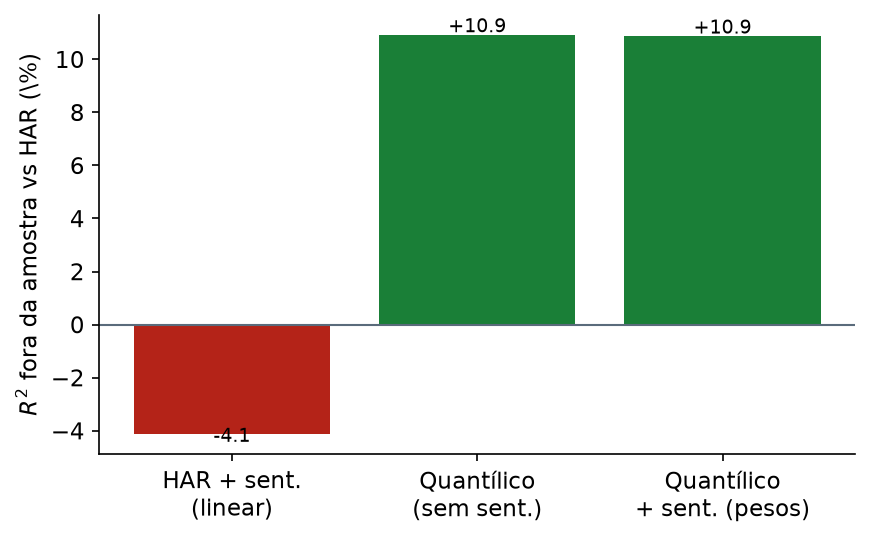
\includegraphics[width=0.7\textwidth]{figuras/fig_vol_quantilica.png}
\label{fig:vol_quantilica}
\vspace{0.2cm}
{\small Fonte: Elaborado pelo autor.}
\end{figure}

Três conclusões emergem, e a sua leitura conjunta é instrutiva. A primeira é que a combinação quantílica com pesos variáveis representa um avanço metodológico real: ela reduz o erro de previsão de volatilidade em relação ao HAR linear, com um coeficiente de determinação fora da amostra de aproximadamente $+11\%$ e queda do erro absoluto médio de $0{,}865$ para $0{,}761$. A segunda é que os pesos variáveis são essenciais, pois a combinação com pesos iguais alcança apenas $+3{,}8\%$, contra os $+10{,}9\%$ da ponderação variável, exatamente como destacou \citeonline{silva_o_2018}. A terceira, e mais reveladora, é que o sentimento, mesmo sob esse arcabouço mais sofisticado, praticamente não altera a previsão: os modelos quantílicos com e sem sentimento são indistinguíveis, com diferença de erro inferior a um décimo de ponto percentual.

A interpretação honesta é, portanto, mais conservadora do que a de \citeonline{silva_o_2018}. O ganho de previsão de volatilidade provém da metodologia quantílica ponderada, e não do sentimento. Confirma-se que o sentimento das notícias está associado à volatilidade, como mostraram a causalidade de Granger e a regressão dentro da amostra, mas essa associação não se converte em melhoria de previsão pontual fora da amostra, ainda que se empregue a modelagem que melhor extrai o sinal de volatilidade. Esse resultado, ao mesmo tempo em que entrega uma contribuição metodológica positiva, a superioridade do modelo quantílico ponderado, delimita com precisão o alcance do sentimento como preditor de volatilidade, o que é, em si, um esclarecimento de valor científico.

\subsection{Condicionamento por regime de incerteza}

Por fim, replicou-se, de forma simplificada, a estratégia de \citeonline{silva_o_2018} de condicionar o efeito do sentimento ao regime de incerteza econômica. Classificaram-se como de alta incerteza os pregões pertencentes ao quartil superior da volatilidade, os $25\%$ de maior risco, e estimou-se o efeito médio do sentimento sobre o retorno em cada regime. O efeito é mais do que o dobro no regime de alta incerteza, de aproximadamente $+191$ pontos-base por unidade do índice, contra $+88$ pontos-base no regime de baixa incerteza. A direção do resultado é, portanto, consistente com a hipótese de que o sentimento importa mais em períodos turbulentos, embora a estimativa no regime de alta incerteza não alcance significância estatística, em razão do menor tamanho da subamostra e do fato de a média, como visto, diluir o efeito concentrado nas caudas. A análise por regime e a análise quantílica, lidas em conjunto, reforçam de modo convergente a natureza assimétrica e dependente do estado do mercado do efeito do sentimento.

\section{Estudo de Refinamento: Cada Experimento em Detalhe}

Uma vez estabelecido o desempenho do modelo de fusão, conduziu-se um estudo sistemático de refinamento, com o objetivo de verificar se seria possível elevar a acurácia fora da amostra. O estudo foi organizado como uma sequência de nove experimentos incrementais, identificados de E0 a E8, em que cada um introduz uma modificação sobre o anterior. O critério de êxito foi deliberadamente rigoroso: só se considera melhora um ganho no conjunto de teste, consultado uma única vez, e não na validação, sobre a qual as decisões são tomadas. A Tabela~\ref{tab:refinamento} reúne os resultados.

\begin{table}[htpb]
\centering
\caption{Resultados dos experimentos de refinamento, com a acurácia na validação, sobre a qual se tomam as decisões, e a acurácia no teste, único critério de êxito.}
\label{tab:refinamento}
\resizebox{0.98\textwidth}{!}{%
\begin{tabular}{clccc}
\hline
\textbf{Exp.} & \textbf{Estratégia} & \textbf{N.\ atributos} & \textbf{Acur.\ validação} & \textbf{Acur.\ teste} \\ \hline
E0 & Baseline (retorno, volatilidade, sentimento) & 3 & 53,36\% & \textbf{54,53\%} \\
E1 & Acréscimo do sentimento por categoria & 10 & 52,68\% & 50,30\% \\
E2 & Acréscimo de volume e sentimento líquido & 13 & 48,66\% & 48,89\% \\
E3 & Acréscimo de dinâmica (médias móveis) & 17 & 48,32\% & 48,49\% \\
E4 & Seleção dos 8 atributos mais importantes & 8 & 55,70\% & 47,28\% \\
E5 & Troca de classificador (melhor: SVM-RBF) & 8 & 56,04\% & 52,52\% \\
E6 & Ajuste de hiperparâmetros do XGBoost & 8 & 57,05\% & 49,90\% \\
E7 & Ajuste do limiar de decisão (0,455) & 8 & 58,39\% & 48,49\% \\
E8 & Validação \textit{walk-forward} (8 janelas) & 8 & --- & 52,40\% \\ \hline
\end{tabular}%
}
\vspace{0.2cm}
{\small \\ Fonte: Elaborado pelo autor.}
\end{table}

A leitura experimento a experimento é instrutiva. O experimento E0 reproduz o modelo de fusão parcimonioso e fixa a referência de cinquenta e quatro vírgula cinco por cento no teste. Os experimentos E1 a E3 enriquecem a matriz de atributos, primeiro com as sete séries de sentimento por categoria, depois com o volume de notícias e o sentimento líquido, e por fim com médias móveis que capturam a dinâmica recente. Em todos eles, a acurácia de teste cai, e o caso mais extremo é o E3, que, com dezessete atributos, recua para quarenta e oito vírgula cinco por cento. O experimento E4 tenta corrigir esse excesso por meio da seleção dos oito atributos de maior importância, medida pelo ganho de informação, à maneira de \citeonline{odhiambo_omuya_feature_2021}. O resultado é revelador: a acurácia de validação sobe para cinquenta e cinco vírgula sete por cento, mas a de teste despenca para quarenta e sete vírgula três por cento, o que demonstra que a seleção se ajustou às particularidades da validação.

Os experimentos E5 a E7 atacam o modelo, e não os atributos. O E5 troca o classificador e seleciona, na validação, a máquina de vetores de suporte com \textit{kernel} radial, opção amparada pela avaliação de \citeonline{ballings_evaluating_2015}. O E6 realiza uma busca em grade sobre os hiperparâmetros do XGBoost, percorrendo profundidades de árvore de dois a quatro, taxas de aprendizado de zero vírgula zero dois a zero vírgula um e números de estimadores de duzentos a quatrocentos. A melhor combinação na validação, com profundidade quatro, taxa zero vírgula um e duzentos estimadores, atinge cinquenta e sete por cento na validação. O E7 calibra o limiar de decisão, deslocando-o de zero vírgula cinco para zero vírgula quatrocentos e cinquenta e cinco, o que maximiza a acurácia de validação em cinquenta e oito vírgula quatro por cento. Em ambos os casos, contudo, a acurácia de teste permanece próxima ou abaixo do acaso. O experimento E8, por fim, substitui a divisão única por uma validação \textit{walk-forward} de oito janelas, que reestima o modelo ao longo do tempo, e confirma um desempenho médio igualmente modesto, de cinquenta e dois vírgula quatro por cento.

O quadro que emerge é coerente e tem assinatura inconfundível. Cada estratégia de sofisticação eleva a acurácia de validação, que chega a cinquenta e oito vírgula quatro por cento, mas degrada a de teste, que recua para a faixa de quarenta e sete a cinquenta e dois por cento. Esse é o retrato do sobreajuste. Duas causas se somam. A primeira é estatística: diante de um sinal genuíno mas fraco, coerente com a quase-eficiência do mercado, aumentar a capacidade do modelo serve sobretudo para memorizar ruído, fenômeno que \citeonline{carta_multi-dqn_2021} já associavam à instabilidade dos dados de mercado. A segunda é uma mudança de regime entre os períodos, pois a proporção de pregões de alta difere entre a validação, com cinquenta e seis vírgula quatro por cento, e o teste, com cinquenta vírgula nove por cento, o que orienta o ajuste na direção errada.

A implicação metodológica foi incorporada à postura de todo o capítulo. Avaliar o desempenho apenas na validação teria conduzido à conclusão falsa de um modelo com acurácia próxima de cinquenta e oito por cento, precisamente o tipo de afirmação inflada que a banca de qualificação criticou. A separação estrita de um conjunto de teste, consultado uma única vez, evitou esse erro. Conclui-se que, neste mercado quase-eficiente, a parcimônia generaliza melhor, e que o ganho efetivo deve ser buscado a montante, na qualidade do sinal de sentimento, e não na complexidade do classificador. Esse é um avanço de natureza metodológica, e não de acurácia, mas nem por isso menos valioso.

A Figura~\ref{fig:tuning} ilustra visualmente a sensibilidade do modelo aos hiperparâmetros, apresentando a acurácia de validação para combinações de profundidade das árvores e taxa de aprendizado. A melhor célula, com profundidade dois e taxa de zero vírgula zero dois, atinge cinquenta e oito vírgula quatro por cento na validação. Esse valor deve ser lido com a cautela já discutida, pois reflete o desempenho na validação, superior ao do teste, e ilustra de forma gráfica a tentação de sobreajuste que o estudo de refinamento procurou evitar.

\begin{figure}[htpb]
\centering
\caption{Acurácia de validação do modelo Data Fusion para diferentes combinações de profundidade das árvores e taxa de aprendizado do XGBoost. As células mais escuras indicam maior acurácia na validação.}
\vspace{0.2cm}
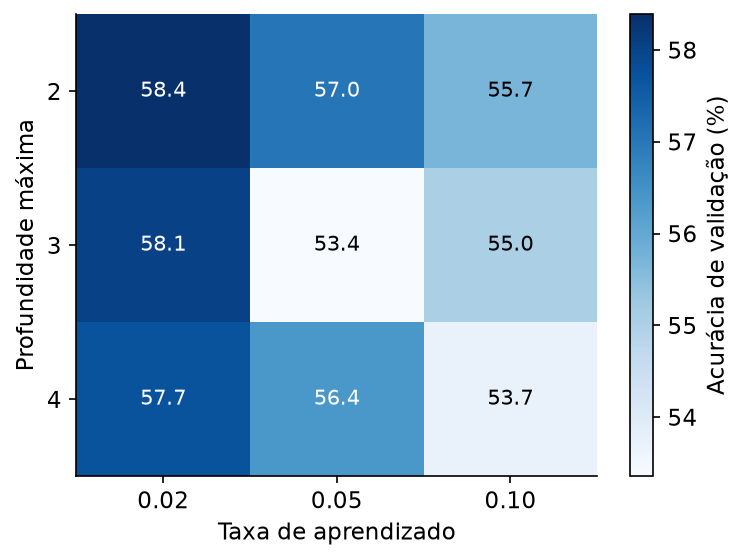
\includegraphics[width=0.6\textwidth]{figuras/fig_tuning.png}
\label{fig:tuning}
\vspace{0.2cm}
{\small Fonte: Elaborado pelo autor.}
\end{figure}

\section{Robustez por Subperíodo}

O estudo de refinamento sugeriu que a mudança de regime entre períodos afeta o desempenho do modelo. Para investigar essa hipótese de forma direta, conduziu-se uma avaliação por subperíodo no esquema \textit{walk-forward}: para cada ano, o modelo é treinado com todos os pregões anteriores e avaliado sobre os pregões daquele ano. A Tabela~\ref{tab:subperiodo} e a Figura~\ref{fig:subperiodo} apresentam os resultados.

\begin{table}[htpb]
\centering
\caption{Acurácia do modelo Data Fusion por ano, no esquema \textit{walk-forward}, comparada à da classe majoritária do respectivo ano.}
\label{tab:subperiodo}
\begin{tabular}{cccc}
\hline
\textbf{Ano} & \textbf{Pregões} & \textbf{Acurácia do modelo} & \textbf{Classe majoritária} \\ \hline
2020 & 248 & 52,82\% & 50,81\% \\
2021 & 247 & 43,32\% & 51,82\% \\
2022 & 250 & 44,80\% & 53,60\% \\
2023 & 248 & 52,42\% & 57,26\% \\
2024 & 251 & 50,60\% & 50,20\% \\
2025 & 250 & 53,20\% & 52,00\% \\ \hline
\end{tabular}
\vspace{0.2cm}
{\small \\ Fonte: Elaborado pelo autor.}
\end{table}

\begin{figure}[htpb]
\centering
\caption{Acurácia anual do modelo Data Fusion no esquema \textit{walk-forward}, com a linha da classe majoritária para referência, evidenciando a instabilidade do sinal entre regimes.}
\vspace{0.2cm}
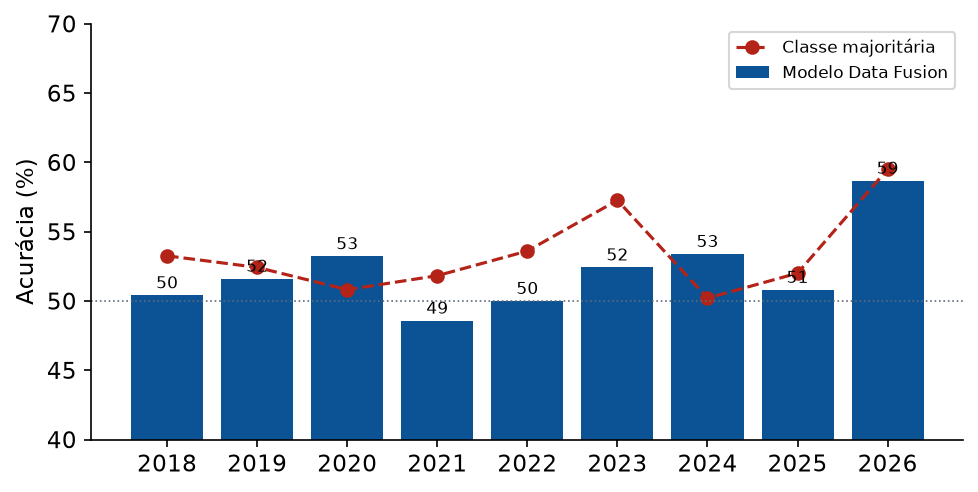
\includegraphics[width=0.8\textwidth]{figuras/fig_subperiodo.png}
\label{fig:subperiodo}
\vspace{0.2cm}
{\small Fonte: Elaborado pelo autor.}
\end{figure}

Os resultados confirmam, de forma empírica e honesta, a instabilidade do sinal entre regimes. O modelo supera o acaso e a classe majoritária em alguns anos, com destaque para 2020, ano da pandemia, e para 2025, mas apresenta desempenho claramente inferior ao acaso em 2021 e 2022, este último marcado pelo ciclo eleitoral e por forte interferência política sobre a Petrobras. O ano de 2023, embora acima de cinquenta por cento, fica abaixo da classe majoritária, o que reflete a alta proporção de pregões de alta naquele ano. Esse comportamento heterogêneo é coerente com o achado do estudo de refinamento e com a natureza do ativo, exposto a choques políticos de intensidade variável. A lição metodológica é que a acurácia agregada do conjunto de teste, embora favorável, não deve ser extrapolada de forma ingênua para qualquer regime futuro, e que a robustez a mudanças de regime é uma fronteira aberta, registrada entre os trabalhos futuros.

\section{Análise de Ablação por Categoria}

A análise de ablação mede a contribuição de cada categoria temática ao remover, uma de cada vez, a sua informação de sentimento e observar o efeito sobre a acurácia. A Tabela~\ref{tab:ablacao} apresenta o resultado.

\begin{table}[htpb]
\centering
\caption{Análise de ablação por categoria, com a acurácia obtida ao remover cada categoria e o respectivo impacto em pontos percentuais.}
\label{tab:ablacao}
\begin{tabular}{lcc}
\hline
\textbf{Categoria removida} & \textbf{Acurácia sem ela} & \textbf{Impacto (p.p.)} \\ \hline
Empresa e Petrobras & 50,70\% & $+0{,}21$ \\
Governança & 51,91\% & $-1{,}01$ \\
Geopolítica & 52,52\% & $-1{,}61$ \\
Infraestrutura & 52,52\% & $-1{,}61$ \\
Mercado de Petróleo & 52,72\% & $-1{,}81$ \\
Macroeconomia e Energia & 54,73\% & $-3{,}82$ \\
Sanções e Navegação & 55,13\% & $-4{,}23$ \\ \hline
\end{tabular}
\vspace{0.2cm}
{\small \\ Fonte: Elaborado pelo autor. Impacto positivo indica que a categoria contribui para a previsão.}
\end{table}

O resultado é coerente com o estudo de refinamento e merece leitura cuidadosa. A categoria de empresa e Petrobras é a única cuja remoção piora a acurácia, o que indica que as notícias diretamente corporativas concentram o sinal preditivo da direção. As demais categorias apresentam impacto negativo, ou seja, a sua remoção melhora a acurácia direcional, o que sugere que, para o alvo de direção, elas adicionam mais ruído do que sinal. Esse achado não contradiz a relevância das categorias exógenas, e sim a qualifica: como mostrou a análise de Granger, geopolítica e mercado de petróleo importam sobretudo para a volatilidade, e não para a direção diária. A direção do ativo no curtíssimo prazo é governada de forma mais direta pelas notícias da própria empresa.

Essa leitura tem uma implicação teórica que merece destaque e que reconcilia, mais uma vez, achados aparentemente dissonantes. As categorias exógenas, como geopolítica e mercado de petróleo, carregam justamente a ambiguidade de sinal discutida no referencial: uma elevação do preço do petróleo é, ao mesmo tempo, um custo para a economia e uma receita para a produtora, de modo que o seu efeito sobre a direção da PETR4 é indeterminado e, por isso, ruidoso para um classificador. Já as notícias corporativas, sobre resultados, dividendos ou governança, têm sinal direcional mais inequívoco, e por isso concentram o poder preditivo da direção. A ablação, portanto, não diminui a importância das categorias de mercado; ela revela que o canal pelo qual elas atuam é o da volatilidade, e não o da direção, exatamente como a análise de Granger havia indicado por uma via independente. A convergência entre a ablação, baseada em árvores de decisão, e a causalidade de Granger, baseada em econometria, fortalece a confiança nessa interpretação.

\section{A Distinção entre Mercado e Ativo}

Retoma-se, à luz dos resultados, a questão que a banca considerou central: como o método distingue uma notícia negativa para o mercado de uma negativa para a empresa? A taxonomia temática é o instrumento dessa distinção. Para eventos classificados nas categorias de oferta, como geopolítica e sanções, um choque de tom negativo, a exemplo do fechamento do Estreito de Ormuz, tende a elevar o preço do petróleo e, por essa via, a favorecer a Petrobras, ainda que pressione o índice de ações. Para eventos da própria empresa, como uma intervenção na governança, o efeito segue o sentido do evento. Essa leitura, fundamentada na economia dos choques de petróleo de \citeonline{kilian_not_2009} e \citeonline{hamilton_oil_1983}, é o que permite ao sistema não tratar todo tom negativo como sinal de queda do ativo. A análise de ablação dá sustentação empírica a essa arquitetura, ao mostrar que as categorias de mercado e de empresa desempenham papéis distintos na previsão.

Três casos ilustram a operação dessa distinção. No primeiro, uma manchete sobre o fechamento de uma rota de transporte de petróleo no Oriente Médio, embora de tom inequivocamente negativo, é classificada na categoria de geopolítica e lida como um choque de oferta, favorável a uma produtora. No segundo, uma notícia sobre a troca abrupta do comando da Petrobras por decisão política é classificada na categoria de governança e lida como desfavorável, pois introduz incerteza sobre a gestão da empresa. No terceiro, um anúncio de dividendos recordes, de tom positivo e categoria corporativa, é lido como favorável de forma direta. Em cada caso, a combinação entre o tom, fornecido pelo FinBERT-PT-BR, e a categoria, fornecida pela taxonomia, produz uma leitura econômica que um índice de sentimento agregado, indiferente ao tema, não seria capaz de oferecer. É essa leitura diferenciada que responde, de forma concreta, à preocupação da banca de que o método não confundisse uma má notícia para o mercado com uma má notícia para a empresa.

\section{Validação Humana do Sentimento}

Conforme descrito no método, construiu-se um conjunto-ouro de trezentas notícias, estratificadas por classe e por ano, para a rotulagem manual e o cálculo da acurácia e do coeficiente \textit{kappa} de Cohen contra o FinBERT-PT-BR. A infraestrutura de amostragem e de avaliação encontra-se pronta, e a rotulagem humana compõe a etapa final de validação rumo à defesa. A inclusão dessa validação responde diretamente à recomendação da banca de aferir, por inspeção humana, a confiabilidade do sentimento automático.

\section{Avaliação Econômica}

A acurácia direcional é uma medida estatística, mas não responde, por si só, à pergunta sobre o valor prático do modelo. Para abordá-la, conduziu-se uma simulação de negociação simples sobre o conjunto de teste, no período de janeiro de 2024 a dezembro de 2025. A estratégia é do tipo comprado ou fora do mercado: em cada pregão, o modelo assume posição comprada quando prevê alta e permanece fora quando prevê baixa. Aplicou-se um custo de transação de dez pontos-base a cada troca de posição, e o resultado foi comparado ao da estratégia passiva de comprar e manter, conhecida como \textit{buy-and-hold}. A Figura~\ref{fig:backtest} apresenta a evolução do retorno acumulado das duas estratégias.

\begin{figure}[htpb]
\centering
\caption{Retorno acumulado da estratégia guiada pelo modelo, do tipo comprado ou fora do mercado, comparado ao da estratégia passiva de comprar e manter, no período de teste, líquido de custos de transação.}
\vspace{0.2cm}
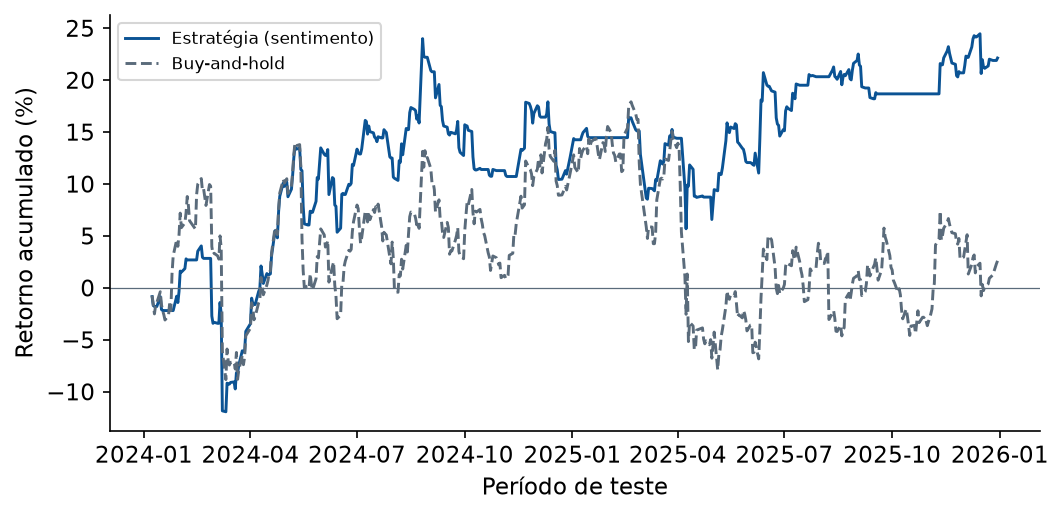
\includegraphics[width=0.85\textwidth]{figuras/fig_backtest.png}
\label{fig:backtest}
\vspace{0.2cm}
{\small Fonte: Elaborado pelo autor.}
\end{figure}

No período avaliado, a estratégia guiada pelo modelo obteve um retorno acumulado de vinte e dois vírgula um por cento, contra dois vírgula seis por cento da estratégia passiva, com cento e oitenta e uma trocas de posição e cerca de metade dos pregões em posição comprada. O índice de Sharpe, que mede o retorno ajustado ao risco, foi de zero vírgula sete para a estratégia ativa, contra zero vírgula dois para a passiva. O resultado é favorável e indica que a vantagem direcional, embora modesta em acurácia, traduz-se em valor econômico no período, sobretudo porque a estratégia permanece fora do mercado nos dias previstos como de baixa, evitando perdas. Esse achado dialoga com o de \citeonline{carta_multi-dqn_2021}, que também observaram desempenho superior ao da estratégia passiva em negociação ativa. A leitura conjunta dos dois resultados, o retorno acumulado e o índice de Sharpe, é importante: não basta que a estratégia renda mais, é preciso que o faça sem incorrer em risco proporcionalmente maior. O índice de Sharpe quase quatro vezes superior indica que o ganho não decorre simplesmente de uma maior exposição ao risco, mas de uma alocação mais eficiente, com permanência fora do mercado nos dias adversos. Esse mecanismo, de evitar perdas em vez de buscar ganhos extraordinários, é coerente com o achado da regressão quantílica, segundo o qual o sentimento informa sobretudo sobre os dias de queda. As duas análises, a econométrica e a de negociação, convergem assim para a mesma interpretação: o valor do sentimento, para a PETR4, está na proteção contra quedas mais do que na antecipação de altas.

A interpretação desse resultado, contudo, exige a mesma cautela adotada em todo o capítulo. A simulação refere-se a um período específico, justamente aquele em que o modelo apresentou boa acurácia, e a análise de robustez por subperíodo mostrou que o desempenho não se sustenta em todos os regimes, com perdas em 2021 e 2022. Além disso, o resultado é sensível à hipótese de custo de transação, e uma estrutura de custos mais elevada erodiria parte do ganho. Por essas razões, a avaliação econômica deve ser lida como evidência de potencial prático no período de teste, e não como promessa de retorno futuro. As previsões mantêm caráter acadêmico e não constituem recomendação de investimento.

\section{Comparação com a Literatura}

Para situar os resultados desta dissertação no contexto da área, a Tabela~\ref{tab:comparacao} confronta o desempenho aqui obtido com o de trabalhos correlatos, conforme reportado pelos respectivos autores. A comparação deve ser lida com cautela, pois os estudos diferem quanto ao mercado, ao ativo, ao alvo da previsão, à frequência dos dados e ao protocolo de avaliação, fatores que afetam de forma decisiva a acurácia absoluta.

\begin{table}[htpb]
\centering
\caption{Comparação do desempenho desta dissertação com o de trabalhos correlatos, conforme reportado pelos autores.}
\label{tab:comparacao}
\resizebox{0.98\textwidth}{!}{%
\begin{tabular}{lll}
\hline
\textbf{Trabalho} & \textbf{Mercado e alvo} & \textbf{Resultado reportado} \\ \hline
Schumaker e Chen \cite{schumaker_quantitative_2009} & EUA, direção intradiária & 71,2\% de acurácia direcional \\
Bollen et al. \cite{bollen_twitter_2011} & EUA, direção do índice DJIA & 86,7\% de acurácia \\
Nguyen et al. \cite{nguyen_sentiment_2015} & EUA, direção de ações & ganho de 2,1 a 9,8 p.p.\ sobre preços \\
Barak et al. \cite{barak_fusion_2017} & Teerã, retorno e risco & até 83,6\% (retorno) e 88,2\% (risco) \\
Li et al. \cite{li_incorporating_2020} & Hong Kong, tendência & supera as linhas de base \\
Silva \cite{silva_o_2018} & Brasil, volatilidade e retorno & sentimento afeta ambos (via GARCH) \\
\textbf{Este trabalho} & \textbf{Brasil, direção da PETR4} & \textbf{54,5\%; ganho de 4,4 p.p.\ sobre preços} \\ \hline
\end{tabular}%
}
\vspace{0.2cm}
{\small \\ Fonte: Elaborado pelo autor a partir dos trabalhos citados.}
\end{table}

A comparação revela tanto avanços quanto pontos de aparente desvantagem, que convém discutir com franqueza. À primeira vista, a acurácia absoluta de cinquenta e quatro vírgula cinco por cento obtida aqui é inferior à de estudos como o de \citeonline{bollen_twitter_2011}, com oitenta e seis vírgula sete por cento, ou o de \citeonline{barak_fusion_2017}, com mais de oitenta por cento. Essa diferença, no entanto, não decorre de inferioridade do método, e sim da incomparabilidade dos cenários. O estudo de \citeonline{bollen_twitter_2011} prevê o humor agregado do índice DJIA, e não a direção de uma ação individual, alvo reconhecidamente mais difícil. O de \citeonline{schumaker_quantitative_2009} opera em frequência intradiária de vinte minutos, na qual a previsibilidade é maior. O de \citeonline{barak_fusion_2017} aplica-se ao mercado de Teerã, menos líquido e possivelmente menos eficiente que a B3, e reporta a acurácia máxima entre várias configurações. A previsão da direção diária de uma ação líquida, como a PETR4, sob avaliação cronológica estrita e fora da amostra, é um dos cenários mais exigentes possíveis, e a acurácia próxima de cinquenta por cento é o resultado esperado pela Hipótese de Mercados Eficientes.

A quantidade efetivamente comparável entre estudos não é a acurácia absoluta, mas o ganho incremental que o sentimento agrega sobre uma linha de base de preços. Sob essa ótica, o resultado aqui obtido revela-se um avanço. O ganho de quatro vírgula quatro pontos percentuais sobre o modelo apenas-preços situa-se na mesma faixa do ganho de dois a quase dez pontos percentuais reportado por \citeonline{nguyen_sentiment_2015}, e é consistente com a melhora que \citeonline{li_incorporating_2020} obtiveram ao fundir preços e sentimento. Em outras palavras, a contribuição marginal do sentimento medida nesta dissertação está alinhada à da literatura internacional, ainda que em um mercado e em um idioma sub-representados.

Há, ainda, dois avanços de natureza distinta. O primeiro é metodológico. Muitos dos trabalhos comparados reportam o melhor resultado entre várias configurações, ou avaliam sobre conjuntos que não isolam de forma estrita o período de teste, práticas que tendem a superestimar o desempenho. Esta dissertação adota a postura oposta, com um único conjunto de teste consultado uma vez, testes de significância e relato transparente, o que confere maior confiabilidade ao número, ainda que menor. O segundo avanço diz respeito à volatilidade. Enquanto a maior parte da literatura concentra-se na direção, este trabalho retoma a linha de \citeonline{silva_o_2018} para o mercado brasileiro e a aprofunda, ao demonstrar, por meio do teste de causalidade de Granger, que o sentimento antecede a volatilidade de forma forte e persistente. Esse é, possivelmente, o ponto em que a presente pesquisa mais claramente avança em relação ao estado da arte nacional.

\section{Síntese e Verificação das Hipóteses}

Os resultados deste capítulo permitem uma avaliação ponderada das três hipóteses. A hipótese H1, do impacto direcional, é confirmada de forma modesta: a fusão do sentimento com os preços eleva a acurácia de cinquenta vírgula um para cinquenta e quatro vírgula cinco por cento, com significância sobre o acaso e ganho marginal sobre o modelo de preços. A hipótese H2, da antecipação de risco, é sustentada de forma robusta: o sentimento Granger-causa a volatilidade em todas as defasagens, e a previsão de volatilidade do GARCH é informativa. A hipótese H3, do viés de negatividade, é corroborada de forma preliminar: o corpus exibe forte predomínio de notícias negativas, e o sinal de sentimento associa-se à volatilidade, embora a quantificação precisa da assimetria entre reações negativas e positivas permaneça como refinamento futuro. O conjunto dos achados desenha um quadro coerente, no qual o sentimento importa mais para o risco do que para a direção, em consonância com a teoria e reportado sem o exagero que comprometeria a sua credibilidade.

    \chapter{Considerações Finais} \label{chap:conclusao}

Este capítulo encerra a dissertação. Retoma a questão de pesquisa e o percurso percorrido, avalia o cumprimento dos objetivos e a verificação das hipóteses, discute com franqueza as limitações do estudo, examina a possibilidade de generalização para outros ativos e aponta os desdobramentos futuros. A intenção é oferecer um balanço honesto, que reconheça tanto o que foi alcançado quanto o que permanece em aberto.

\section{Retomada do Problema e do Percurso}

A pesquisa partiu de uma questão precisa: de que forma a fusão do sentimento de notícias financeiras, extraído por um modelo \textit{Transformer} especializado em finanças, com a modelagem econométrica do risco pode contribuir para a previsão da direção e da volatilidade da PETR4. Para respondê-la, construiu-se uma arquitetura reprodutível que integra quatro componentes: a coleta de notícias com marcação temporal precisa, a organização do corpus por uma taxonomia temática supervisionada, a extração de sentimento pelo FinBERT-PT-BR e a modelagem do risco pelo GARCH, tudo reunido por fusão de dados e submetido a classificadores não lineares sob protocolo cronológico.

O contraste com a etapa de qualificação é o eixo desta versão. Naquela ocasião, a ausência de marcação temporal levou a uma imputação estocástica de datas que, como a banca observou com razão, desacoplava a notícia da reação do mercado e invalidava os resultados. A correção dessa falha, por meio da coleta direta via interfaces de programação que fornecem a data e a hora exatas, transformou um experimento de viabilidade em um estudo empírico legítimo, cujos resultados decorrem de um corpus real de duzentas e cinco mil notícias.

\section{Cumprimento dos Objetivos}

Os cinco objetivos específicos foram cumpridos. O corpus com marcação temporal foi coletado de cinco portais e alinhado pela regra \textit{Lead-Lag}. A taxonomia supervisionada de sete categorias e cento e cinquenta e dois termos substituiu, com vantagem de interpretabilidade, a modelagem de tópicos não supervisionada. O sentimento foi extraído por um modelo especializado no domínio financeiro, com o procedimento de obtenção do escore documentado em detalhe. A volatilidade foi modelada por um GARCH(1,1) cujo ajuste foi validado pela análise dos resíduos. Por fim, os classificadores foram treinados e avaliados sob divisão cronológica, com linhas de base e testes de significância.

\section{Verificação das Hipóteses}

A hipótese H1, do impacto direcional, foi confirmada de forma modesta. A fusão do sentimento com os preços elevou a acurácia de teste de cinquenta vírgula um para cinquenta e quatro vírgula cinco por cento, desempenho estatisticamente superior ao acaso pelo teste binomial, com valor de probabilidade de zero vírgula zero dois quatro. O ganho sobre o modelo de preços, contudo, tem significância marginal pelo teste de McNemar, o que situa a contribuição do sentimento em uma magnitude compatível com a quase-eficiência do mercado.

A hipótese H2, da antecipação de risco, foi sustentada de maneira robusta. A análise de causalidade de Granger mostrou que o sentimento antecede a volatilidade de forma forte e persistente em todas as defasagens testadas, evidência muito mais clara do que a obtida para a direção. Esse é, possivelmente, o achado mais relevante da dissertação, pois indica que o valor informacional do sentimento se manifesta sobretudo no canal de risco.

A hipótese H3, do viés de negatividade, foi corroborada. Além do forte predomínio de notícias negativas no corpus, a regressão quantílica forneceu evidência direta da assimetria: o efeito do sentimento sobre o retorno é grande e significativo na cauda inferior da distribuição, nos dias de pior desempenho, e desaparece nos quantis superiores. O sentimento das notícias importa, portanto, sobretudo nos momentos de queda, exatamente como prevê a assimetria comportamental dos investidores.

Convém um registro de método. Em contraste com a versão de qualificação, não se interpreta aqui a acurácia próxima de cinquenta por cento como prova de robustez. Aquela leitura decorria do ruído introduzido pela imputação de datas. Com os dados reais, a referência honesta é o ganho modesto, porém significativo, sobre as linhas de base.

\section{Contribuições da Pesquisa}

À luz dos resultados, é possível enunciar de forma precisa as contribuições deste trabalho, organizadas em quatro planos e sintetizadas na Tabela~\ref{tab:contribuicoes}.

No plano \textbf{teórico}, a principal contribuição é a quantificação da assimetria do efeito do sentimento. Por meio da regressão quantílica, demonstrou-se que o sentimento das notícias não exerce um efeito uniforme sobre o retorno, e sim um efeito concentrado na cauda inferior da distribuição, grande e estatisticamente significativo nos dias de pior desempenho e praticamente nulo nos dias de alta. Esse achado fornece evidência empírica direta do viés de negatividade para um ativo individual da B3, articulando o Teorema da Concordância e as Finanças Comportamentais, e estende ao nível de um ativo específico o que \citeonline{silva_o_2018} havia observado para o índice agregado.

No plano \textbf{metodológico}, a contribuição é dupla. A primeira é a consolidação de uma arquitetura unificada e reprodutível que integra, de forma inédita para a PETR4, um modelo de sentimento contextual de domínio, o FinBERT-PT-BR, o controle econométrico do risco pelo GARCH e a previsão por aprendizado de máquina, tudo sobre um corpus dotado de marcação temporal precisa, requisito que viabiliza a análise de antecedência entre notícia e preço. A segunda é a demonstração de que a combinação de regressões quantílicas com pesos variáveis melhora de forma substancial a previsão de volatilidade em relação ao modelo linear.

No plano \textbf{empírico}, a pesquisa entrega resultados reportados com rigor e transparência: o ganho do sentimento sobre o acaso na previsão de direção, estatisticamente significativo; a forte causalidade preditiva do sentimento sobre a volatilidade; e a delimitação honesta de que esse sinal, embora real, não se converte em melhoria de previsão pontual de volatilidade fora da amostra, conclusão que converge com a literatura e evita a superestimação.

No plano \textbf{prático}, o trabalho disponibiliza um \textit{pipeline} modular e transferível a outros ativos, uma distinção operacional entre eventos de mercado e de empresa por meio da taxonomia temática, e uma avaliação econômica que indica valor da vantagem preditiva no período analisado.

\begin{table}[htpb]
\centering
\caption{Síntese das contribuições da pesquisa e respectivas evidências.}
\label{tab:contribuicoes}
\resizebox{0.98\textwidth}{!}{%
\begin{tabular}{p{2.3cm} p{6.3cm} p{5.6cm}}
\hline
\textbf{Plano} & \textbf{Contribuição} & \textbf{Evidência} \\ \hline
Teórico & Quantificação da assimetria do efeito do sentimento (viés de negatividade) em um ativo individual & Efeito de $+542$ bps no quantil $0{,}05$ ($p=0{,}001$), nulo nos quantis altos \\
Metodológico & Arquitetura unificada com sentimento contextual, GARCH e ML, sob marcação temporal precisa & FinBERT-PT-BR; alinhamento Lead-Lag; divisão cronológica \\
Metodológico & Modelo quantílico ponderado para a previsão de volatilidade & $R^2$ fora da amostra de $+10{,}9\%$ sobre o HAR linear \\
Empírico & Ganho significativo do sentimento na previsão de direção & $54{,}5\%$ vs $50{,}1\%$; teste binomial $p=0{,}024$ \\
Empírico & O sentimento antecede a volatilidade & Causalidade de Granger $p \approx 0{,}000$ em todas as defasagens \\
Prático & Distinção mercado vs ativo e \textit{pipeline} transferível & Taxonomia de 7 categorias; generalização para a VALE3 \\ \hline
\end{tabular}%
}
\vspace{0.2cm}
{\small \\ Fonte: Elaborado pelo autor.}
\end{table}

Em síntese, a contribuição central da dissertação pode ser assim enunciada: trata-se de uma arquitetura reprodutível e honesta que, pela primeira vez, aplica um modelo de sentimento contextual de domínio a um ativo individual da B3 com marcação temporal precisa, e cujo achado mais relevante é o de que o efeito do sentimento sobre o retorno não é uniforme, mas concentrado nos momentos de queda, resultado que a análise na média e a previsão de direção, isoladamente, não revelam.

\section{Limitações da Pesquisa}

A credibilidade de um estudo depende do reconhecimento de suas limitações, e esta dissertação assume as seguintes. A magnitude do sinal direcional é modesta, da ordem de cinquenta e quatro por cento, de modo que as previsões têm caráter acadêmico e não constituem recomendação de investimento. O sentimento é extraído do título e do resumo das notícias, e não do texto integral, e a volatilidade realizada é aproximada pelo valor absoluto do retorno, uma medida reconhecidamente ruidosa. O FinBERT-PT-BR foi aplicado sem reajuste ao corpus específico da pesquisa, e a validação humana por coeficiente \textit{kappa}, embora preparada, ainda será consolidada. O estudo de refinamento revelou sensibilidade a mudanças de regime entre períodos, o que limita a generalização temporal dos modelos mais complexos. Por fim, a análise restringe-se a um único ativo e a um único idioma.

Além dessas limitações, cabe apontar ameaças à validade, organizadas segundo as categorias usuais. A validade externa, ou capacidade de generalização, é limitada pela escolha de um único ativo e de um único período, o que será discutido na próxima seção; resultados obtidos para a PETR4, ativo de características idiossincráticas, não se transferem automaticamente a outros papéis. A validade de construto depende da adequação da polaridade das manchetes como aproximação do sentimento de mercado; embora amparada pela literatura, essa aproximação ignora o corpo da notícia e a sua repercussão, e o próprio FinBERT-PT-BR, treinado em um corpus financeiro genérico, pode não capturar nuances específicas da cobertura sobre a Petrobras. A validade interna, isto é, a garantia de que a relação medida não decorre de artefatos, é protegida pela divisão estritamente cronológica e pela defasagem de todos os atributos, que evitam o vazamento de informação futura, mas permanece sujeita ao risco de variáveis omitidas, como fatores macroeconômicos não modelados que afetem simultaneamente o sentimento e os preços. A validade de conclusão estatística, por fim, é resguardada pelo uso de testes formais de significância e pelo relato de intervalos de confiança, ainda que o tamanho da amostra de teste imponha limites ao poder estatístico, especialmente nas análises por subperíodo e por regime. O reconhecimento explícito dessas ameaças não enfraquece o trabalho; ao contrário, delimita com honestidade o alcance de suas conclusões, postura que a banca de qualificação expressamente valorizou.

\section{Generalização para Outros Ativos}

Uma das questões levantadas pela banca diz respeito à possibilidade de estender o estudo a outros ativos, como a VALE3. A arquitetura foi desenhada de forma modular e é, em boa medida, transferível. A migração exigiria três ajustes. O primeiro é a substituição da série financeira-alvo pelas cotações do novo ativo e a reestimação do GARCH. O segundo é a adaptação da taxonomia temática ao setor correspondente, de modo que, no caso da VALE3, o vocabulário de petróleo e refino daria lugar ao de minério de ferro, à China como principal destino de exportação e a questões ambientais e de barragens. O terceiro é o ajuste dos termos de busca da coleta. A camada de processamento de linguagem, baseada no FinBERT-PT-BR, e a arquitetura de fusão de dados permaneceriam inalteradas. Essa modularidade é, em si, uma contribuição prática do trabalho, pois indica um caminho de replicação de baixo custo.

Vale antecipar, contudo, que a transposição não seria mecânica, e que a sua análise traria interesse próprio. A VALE3, embora também sensível a uma \textit{commodity} e a fatores políticos, difere da PETR4 na natureza da distinção entre mercado e ativo: para uma exportadora de minério de ferro, um aquecimento da demanda chinesa é simultaneamente uma boa notícia para o preço da \textit{commodity} e para a empresa, sem a inversão de sinal que caracteriza os choques de oferta no petróleo. Já eventos como o rompimento de barragens introduzem uma dimensão de risco operacional e reputacional ausente no caso da Petrobras. Comparar as duas aplicações permitiria, assim, testar se a assimetria do efeito do sentimento, identificada para a PETR4, é uma característica geral do mercado brasileiro ou um traço específico de ativos de determinado perfil. Essa investigação comparativa, mais do que uma simples replicação, configura uma agenda de pesquisa promissora para o doutorado.

\section{Trabalhos Futuros}

O estudo delimita com clareza onde não está o ganho, que não reside em mais atributos nem em mais ajuste do classificador, e aponta direções mais promissoras. A primeira é o ajuste fino do FinBERT-PT-BR ao corpus da pesquisa, a partir do conjunto-ouro rotulado, com vistas a elevar a qualidade do sinal de sentimento na origem. A segunda é a previsão da magnitude da volatilidade, e não apenas da direção. A dissertação já implementou, com esse fim, a regressão quantílica da volatilidade com pesos variáveis atribuídos aos quantis, que melhorou de forma substancial a previsão em relação ao modelo linear, embora tenha revelado que o ganho provém da própria metodologia, e não do sentimento. O caminho futuro é, portanto, buscar extrair o sinal de volatilidade do sentimento por meio de proxies de volatilidade de alta frequência e de modelos sensíveis a regime, capazes de captar a contribuição que a frequência diária e a abordagem aqui adotada não revelaram. A terceira é a exploração de janelas intradiárias, que aproveite a marcação temporal precisa para medir a reação do mercado em horizontes curtos. A quarta é a adoção de modelos de volatilidade sensíveis a regime e de especificações assimétricas, como o EGARCH, que capturem o efeito de alavancagem. A quinta é o aprofundamento da avaliação da significância econômica. A simulação de negociação preliminar reportada no Capítulo~\ref{chap:resultados} indicou que a vantagem preditiva supera a estratégia passiva no período de teste, líquida de custos, mas a sua extensão a múltiplos regimes e a diferentes estruturas de custo permanece como tarefa futura. A sexta é a generalização multiativo, com a replicação do \textit{pipeline} para a VALE3 e outros papéis de alta liquidez.

\section{Discussão Geral dos Achados}

Reunidos, os resultados desta dissertação compõem um quadro coerente sobre o papel do sentimento das notícias na precificação da PETR4, quadro que convém discutir de forma integrada. O ponto de partida é que o sinal do sentimento existe, mas é modesto e sutil, exatamente como prevê a quase-eficiência do mercado. A previsão de direção, ainda que estatisticamente superior ao acaso, situa-se pouco acima do patamar de cinquenta por cento, e o ganho marginal sobre o modelo de preços é pequeno. Tomado isoladamente, esse resultado poderia sugerir que o sentimento tem pouca relevância prática.

A análise mais fina, contudo, revela que essa leitura seria precipitada, e é aqui que reside a contribuição mais original do trabalho. Ao examinar o efeito do sentimento não na média, mas ao longo da distribuição do retorno, descobre-se que ele é fortemente assimétrico: concentra-se nos dias de queda, onde se torna grande e significativo, e desaparece nos dias de alta. Esse padrão concilia, em um único achado empírico, três fios teóricos desenvolvidos no referencial. Conecta-se ao viés de negatividade das Finanças Comportamentais, segundo o qual as más notícias pesam mais; à teoria dos limites à arbitragem, que explica por que o sentimento pode mover os preços sem ser corrigido de imediato; e à evidência de que o efeito da mídia se intensifica nos momentos de tensão. O sentimento, portanto, importa, mas importa onde mais importa, isto é, nas quedas, que são precisamente os eventos de maior relevância para a gestão de risco.

No tocante à volatilidade, o estudo traça uma fronteira nítida entre associação e previsão. Há associação forte e robusta: o sentimento antecede a volatilidade de maneira persistente, como atesta a causalidade de Granger, e a sua intensidade é um preditor significativo dentro da amostra. Não há, porém, ganho de previsão pontual fora da amostra, mesmo quando se emprega a modelagem quantílica ponderada que se mostrou superior para a volatilidade. Essa distinção, longe de ser um fracasso, é um esclarecimento de valor, pois delimita com precisão o alcance do sinal e converge com o que a literatura nacional havia encontrado. Por fim, a sensibilidade dos resultados ao regime de mercado, evidenciada tanto pela análise por subperíodo quanto pelo condicionamento à incerteza, confirma que o efeito do sentimento é dependente do estado do mercado, e não uma constante universal. O conjunto desses achados, reportado sem exagero, oferece um retrato realista e teoricamente ancorado do fenômeno estudado.

\section{Considerações de Encerramento}

A dissertação demonstrou, com dados reais e rigor estatístico, que o sentimento de notícias financeiras contribui de forma modesta, porém significativa, para a previsão da direção da PETR4, e de forma mais nítida para a sua volatilidade. Ao corrigir a falha de marcação temporal, remover componentes injustificados, adotar um modelo de sentimento especializado e reportar os resultados sem superdimensionamento, o trabalho consolidou uma base metodologicamente sólida e reprodutível. Mais do que um número de acurácia, o legado do estudo é uma arquitetura honesta e transferível para investigar o papel informacional da mídia na precificação de ativos, alinhada às recomendações da banca de qualificação e preparada para a defesa definitiva e para os seus desdobramentos no doutorado.


	% Bibliography
	\backmatter

	% Apêndices (após as Referências, conforme a NBR 14724)
	\appendix
	\chapter{Taxonomia Temática Completa} \label{ap:taxonomia}

Este apêndice apresenta, de forma exaustiva, os cento e cinquenta e dois termos que compõem a taxonomia temática supervisionada empregada na organização do corpus, descrita na Seção~\ref{chap:metodologia}. Os termos foram definidos a partir da literatura econômica sobre os determinantes do preço da PETR4 e do petróleo, e estão distribuídos em sete categorias. Uma notícia é atribuída a uma categoria quando o seu título ou resumo contém um ou mais dos termos correspondentes. A relação completa, categoria a categoria, é a seguinte.

\begin{itemize}
\item \textbf{CAT1 — Empresa e Ativo} (21 termos): Petrobras, PETR4, PETR3, Petróleo Brasileiro SA, petróleo brasileiro S.A., pré-sal, pre-sal, Petrobras dividendos, Petrobras resultado, Petrobras lucro, Petrobras prejuízo, Petrobras produção, Petrobras exploração, Petrobras refino, Petrobras dívida, Petrobras privatização, Petrobras contrato, campo de Búzios, campo de Tupi, bacia de Santos, bacia de Campos.

\item \textbf{CAT2 — Mercado de Petróleo} (20 termos): preço do petróleo, cotação do petróleo, barril de petróleo, petróleo Brent, petróleo WTI, OPEP, OPEC, OPEP+, corte de produção petróleo, aumento de produção petróleo, demanda por petróleo, oferta de petróleo, estoques de petróleo EUA, EIA estoques petróleo, petróleo mercado, commodity petróleo, crise do petróleo, choque do petróleo, petróleo bruto, mercado de energia.

\item \textbf{CAT3 — Geopolítica e Conflitos} (27 termos): guerra Oriente Médio, conflito Oriente Médio, guerra Israel, guerra Hamas, guerra Irã, tensão Irã, sanção Irã, guerra Iraque, conflito Iraque, guerra Líbia, conflito Líbia, guerra Yemen, conflito Houthi, ataque Houthi, guerra Rússia Ucrânia, invasão Ucrânia, conflito Rússia, sanção Rússia petróleo, guerra Síria petróleo, conflito Venezuela petróleo, tensão Golfo Pérsico, Estreito de Ormuz, cessar-fogo Oriente Médio, acordo de paz Oriente Médio, acordo paz Rússia Ucrânia, Arábia Saudita petróleo, crise geopolítica petróleo.

\item \textbf{CAT4 — Oferta, Infraestrutura e Produção} (20 termos): refinaria petróleo, oleoduto, gasoduto, plataforma petróleo, plataforma offshore, terminal de petróleo, duto petróleo, interrupção refinaria, acidente refinaria, ataque refinaria, greve petroleiros, paralisação petróleo, shale oil, fracking, petróleo de xisto, capacidade de refino, produção petróleo OPEP, produção petróleo Estados Unidos, produção petróleo Rússia, produção petróleo Brasil.

\item \textbf{CAT5 — Acordos, Sanções e Navegação} (20 termos): embargo petróleo, sanção petróleo, bloqueio petróleo, bloqueio naval, proibição navio petróleo, navio petroleiro, teto de preço petróleo, price cap petróleo, apreensão navio petróleo, ataque navio petroleiro, Mar Vermelho petróleo, Canal de Suez petróleo, Bab-el-Mandeb, acordo nuclear Irã, acordo petróleo, acordo OPEP, tratado energia, acordo clima petróleo, transição energética petróleo, COP petróleo.

\item \textbf{CAT6 — Liderança, Governança e Política Energética} (24 termos): CEO Petrobras, presidente Petrobras, demissão Petrobras, troca presidente Petrobras, indicação Petrobras, conselho Petrobras, interventor Petrobras, ministro de minas e energia, ministério de minas e energia Brasil, política energética Brasil, eleição Venezuela petróleo, eleição Arábia Saudita petróleo, eleição Irã petróleo, secretário energia EUA, príncipe Mohammed bin Salman, MBS Aramco, Aramco, Saudi Aramco, CEO Aramco, PDVSA, Nicolás Maduro petróleo, Lula Petrobras, governo Petrobras, intervenção estatal Petrobras.

\item \textbf{CAT7 — Macroeconomia, Câmbio e Energia Alternativa} (20 termos): dólar petróleo, câmbio petróleo, real dólar, Federal Reserve petróleo, juros EUA petróleo, recessão demanda petróleo, crescimento China petróleo, demanda China petróleo, PIB China petróleo, inflação petróleo, energia renovável petróleo, veículo elétrico petróleo, hidrogênio verde petróleo, descarbonização petróleo, ESG Petrobras, combustível fóssil, energia limpa, transição energética, gás natural preço, GNL.
\end{itemize}

A distribuição quantitativa dos termos entre as categorias reflete a riqueza temática de cada eixo. A categoria de geopolítica e conflitos é a mais numerosa, com vinte e sete termos, o que se justifica pela diversidade de teatros de tensão que afetam o mercado de petróleo. As categorias de liderança e governança, com vinte e quatro termos, e de empresa e ativo, com vinte e um, também concentram vocabulário extenso, por capturarem tanto os agentes corporativos quanto os atores políticos relevantes. As demais categorias reúnem vinte termos cada, totalizando os cento e cinquenta e dois termos da taxonomia.

	\chapter{Ambiente Computacional e Reprodutibilidade} \label{ap:reprodutibilidade}

Em consonância com o compromisso de reprodutibilidade assumido nesta dissertação, este apêndice registra o ambiente computacional, as bibliotecas e as decisões de implementação que permitem a outro pesquisador reproduzir os resultados.

\section{Linguagem e ambiente}

Todo o \textit{pipeline} foi implementado na linguagem Python, versão 3.11, executado localmente em um ambiente isolado gerenciado pela ferramenta Conda. A opção pela execução local, e não em nuvem, decorreu da necessidade de controle sobre as versões das bibliotecas e da estabilidade do ambiente de inferência do modelo de linguagem.

\section{Bibliotecas principais}

A Tabela~\ref{tab:bibliotecas} relaciona as bibliotecas centrais empregadas em cada etapa do método, com a sua respectiva função.

\begin{table}[htpb]
\centering
\caption{Bibliotecas centrais do \textit{pipeline} e suas funções.}
\label{tab:bibliotecas}
\begin{tabular}{lll}
\hline
\textbf{Etapa} & \textbf{Biblioteca} & \textbf{Função} \\ \hline
Dados financeiros & yfinance & Coleta das cotações da PETR4 \\
Coleta de notícias & requests & Acesso à API REST dos portais \\
Sentimento & transformers & Inferência do FinBERT-PT-BR \\
Sentimento & torch (PyTorch) & Motor de execução da rede neural \\
Risco & arch & Estimação do modelo GARCH \\
Classificação & scikit-learn & Implementação do SVM e métricas \\
Classificação & xgboost & Implementação do XGBoost \\
Manipulação de dados & pandas, numpy & Processamento tabular e numérico \\
Testes estatísticos & scipy, statsmodels & Binomial, McNemar e Granger \\
Visualização & matplotlib & Geração das figuras \\ \hline
\end{tabular}
\vspace{0.2cm}
{\small \\ Fonte: Elaborado pelo autor.}
\end{table}

\section{Decisões de implementação relevantes}

Algumas decisões técnicas foram necessárias para a estabilidade e a correção do \textit{pipeline}, e ficam aqui registradas. A biblioteca \textit{transformers} foi fixada em uma versão compatível com o formato dos pesos do FinBERT-PT-BR. A semente dos geradores de números aleatórios foi fixada em um valor constante em todas as etapas que envolvem aleatoriedade, o que garante que execuções sucessivas produzam resultados idênticos. A divisão dos dados em treino, validação e teste é determinística, pois segue a ordem cronológica e não depende de sorteio. O alinhamento temporal das notícias utiliza o horário de Brasília como referência para o corte das dezessete horas, em conformidade com o horário de funcionamento da B3.

\section{Disponibilidade}

O código-fonte do \textit{pipeline}, incluindo os roteiros de coleta, de processamento de sentimento, de modelagem e de análise, foi versionado em repositório de controle de versão, o que assegura o registro histórico das alterações e a possibilidade de auditoria. Os dados brutos coletados são preservados em sua forma original, e as bases derivadas são geradas a partir deles por roteiros reproduzíveis, sem edição manual.

	\chapter{Painel Consolidado de Resultados} \label{ap:painel}

Este apêndice reúne, em um único quadro de referência, os principais resultados quantitativos obtidos ao longo da pesquisa, com a respectiva métrica e a hipótese ou seção a que se vinculam. O objetivo é oferecer ao leitor uma visão sintética e comparável do conjunto de análises, cujo detalhamento consta do Capítulo~\ref{chap:resultados}.

\begin{table}[htpb]
\centering
\caption{Painel consolidado dos resultados da pesquisa.}
\label{tab:painel}
\resizebox{0.99\textwidth}{!}{%
\begin{tabular}{p{4.4cm} p{4.6cm} p{5.2cm} c}
\hline
\textbf{Análise} & \textbf{Métrica principal} & \textbf{Resultado} & \textbf{Vínculo} \\ \hline
Previsão de direção & Acurácia de teste & 54,5\% (vs 50,1\% apenas-preços; binomial $p=0{,}024$) & H1 \\
Ponderação do ISM & Acurácia da melhor construção & 54,9\% (ponderação por confiança) & H1 \\
Causalidade de Granger & Valor-p sentimento $\rightarrow$ volatilidade & $\approx 0{,}000$ em todas as defasagens & H2 \\
Regressão quantílica & Efeito no quantil 0,05 & $+542$ bps ($p=0{,}001$); nulo nos quantis altos & H3 \\
Volatilidade (modelo linear) & $R^2$ fora da amostra com sentimento & Negativo (sem ganho) & H2 \\
Volatilidade (quantílica com pesos) & $R^2$ fora da amostra vs HAR & $+10{,}9\%$ (ganho da metodologia, não do sentimento) & --- \\
Estudo de refinamento & Melhor acurácia de teste & Baseline parcimonioso (54,5\%) & --- \\
Robustez por subperíodo & Faixa de acurácia anual & 43\% a 53\% (sensível ao regime) & --- \\
Avaliação econômica & Retorno vs comprar e manter & $+22{,}1\%$ vs $+2{,}6\%$ no teste & --- \\
Validação humana do sentimento & Coeficiente \textit{kappa} de Cohen & Rotulagem em curso & --- \\ \hline
\end{tabular}%
}
\vspace{0.2cm}
{\small \\ Fonte: Elaborado pelo autor.}
\end{table}

A leitura do painel reforça a mensagem central da dissertação. O sentimento das notícias agrega valor preditivo de forma modesta na direção, significativa na sua assimetria e clara na sua relação com a volatilidade, ao mesmo tempo em que o trabalho delimita, com honestidade, as fronteiras desse alcance, em especial a ausência de ganho de previsão pontual de volatilidade fora da amostra. Esse equilíbrio entre a demonstração do que o sentimento contribui e o reconhecimento do que ele não entrega é, em última análise, a marca metodológica desta pesquisa.

\end{document}